\documentclass[12pt,english,fleqn,openany,letterpaper,pagesize, ]{scrbook}

\usepackage[utf8]{inputenc}
\usepackage[english]{babel}%escribir con acentos sin necesidad de comandos \'{} .
\usepackage{fancyhdr}
\usepackage{fancyhdr}
\usepackage{epic}
\usepackage{eepic}
\usepackage[fleqn]{amsmath}
\usepackage{threeparttable}
\usepackage{amscd}
\usepackage{amsmath}
\usepackage{here}
\usepackage{xcolor}
\definecolor{darkblue}{rgb}{0.0,0.0,0.45}
\usepackage[colorlinks=true,allcolors=black,urlcolor=darkblue]{hyperref}
\usepackage{romannum}
\usepackage{listings}
\usepackage{graphicx}
\usepackage{lscape}
\usepackage{amssymb}
\usepackage{tabularx}
\usepackage{tensor}
\usepackage{subfigure}
\usepackage{longtable}
\usepackage{braket}
%\usepackage{natbib}
\usepackage[backend=bibtex,style=ieee,natbib=true]{biblatex}
\usepackage{mathtools}
\usepackage{multirow}
\usepackage{booktabs}
%\usepackage{cite} % Add this line for citations
%\bibpunct{(}{)}{;}{a}{}{,} % to follow the A&A style


\usepackage{csquotes}
%Code listing style named "mystyle"
\lstdefinestyle{mystyle}{
  backgroundcolor=\color{backcolour}, commentstyle=\color{bondiblue},
  keywordstyle=\color{codegreen},
  numberstyle=\tiny\color{codegray},
  stringstyle=\color{bostonuniversityred},
  basicstyle=\ttfamily\footnotesize,
  breakatwhitespace=false,         
  breaklines=true,                 
  captionpos=b,                    
  keepspaces=true,                 
  numbers=left,                    
  numbersep=4pt,                  
  showspaces=false,                
  showstringspaces=false,
  showtabs=true,                  
  tabsize=2
}


\usepackage{rotating} %Para rotar texto, objetos y tablas seite. No se ve en DVI solo en PS. Seite 328 Hundebuch
                        %se usa junto con \rotate, \sidewidestable ....


\renewcommand{\theequation}{\thechapter-\arabic{equation}}
\renewcommand{\thefigure}{\textbf{\thechapter-\arabic{figure}}}
\renewcommand{\thetable}{\textbf{\thechapter-\arabic{table}}}


\pagestyle{fancyplain}%\addtolength{\headwidth}{\marginparwidth}
\textheight22.5cm \topmargin0cm \textwidth16.5cm 

\oddsidemargin0.0cm \evensidemargin0.0cm%
\renewcommand{\chaptermark}[1]{\markboth{\thechapter\; #1}{}}
\renewcommand{\sectionmark}[1]{\markright{\thesection\; #1}}
\lhead[\fancyplain{}{\thepage}]{\fancyplain{}{\rightmark}}
\rhead[\fancyplain{}{\leftmark}]{\fancyplain{}{\thepage}}
\fancyfoot{}
\thispagestyle{fancy}%


\addtolength{\headwidth}{0cm}
\unitlength0mm %Define la unidad LE para Figuras
\mathindent6cm %Define la distancia de las formulas al texto,  fleqn las descentra
\marginparwidth0cm
\parindent0cm %Define la distancia de la primera linea de un parrafo a la margen

%Para tablas,  redefine el backschlash en tablas donde se define la posici\'{o}n del texto en las
%casillas (con \centering \raggedright o \raggedleft)
\newcommand{\PreserveBackslash}[1]{\let\temp=\\#1\let\\=\temp}
\let\PBS=\PreserveBackslash

%Espacio entre lineas
\renewcommand{\baselinestretch}{1.5}

%Neuer Befehl f\"{u}r die Tabelle Eigenschaften der Aktivkohlen
\newcommand{\arr}[1]{\raisebox{1.5ex}[0cm][0cm]{#1}}

%Neue Kommandos
\usepackage{Befehle}
%Inicio del documento. Tener en cuenta que hay archivos auxiliares
\addbibresource{BibliMSc,Kap1/BibtexChap1,Kap2/BibtexChap2,Kap3/BibtexChap3,Kap4/BibtexChap4,Kap5/BibtexChap5,Kap6/BibtexChap6,Kap7/BibtexChap7,Kap8/BibtexChap8}

\begin{document}
%\newpage
%\setcounter{page}{1}

\begin{center}
\begin{figure*}
    \centering%
    
\includegraphics[scale=0.35]{HojaTitulo/Figures_HojaTitulo/Universidad_de_los_Andes_(logo).png} % Replace \epsfig with \includegraphics and remove the ".eps" extension
\end{figure*}
\thispagestyle{empty} \vspace*{2.0cm} \textbf{\LARGE
The Thorium fuel cycle in nuclear reactors}\\[2.5cm]

\Large\textbf{Frank Worman Garcia Eslava}\\[2.0cm]

Advisor: PhD. Juan Carlos Sanabria Arenas \\[2.0cm]


\Large Thesis presented to obtain the degree of Physicist \\ [2.0cm]


Bogot\'{a}, Colombia\\ [0.5cm]
\today \\
\end{center}

\newpage{\pagestyle{empty}\cleardoublepage}

\newpage
\thispagestyle{empty} \textbf{}\normalsize
\\\\\\%
\textbf{\LARGE Agradecimientos}\\
\addcontentsline{toc}{chapter}{Agradecimientos}

Quisiera comenzar agradeciendo a Dios y a mi familia por su amor, apoyo y paciencia durante todo este tiempo. A mi madre, por ser mi fuente de inspiración y por brindarme siempre su amor incondicional. A mi padre, por su sabiduría y su ejemplo de trabajo duro y dedicación, enseñándome el valor del esfuerzo constante. Ambos padres me han dado amor incondicional y son mi fuente de inspiración.

A mi hermana, primos y tíos por su apoyo, escucha y amor. En especial, a mis primos Jefferson y Yeiri, y a mi tía Jesusa, por estar siempre presentes y ser un pilar fundamental en mi vida.

A mis profesores, quienes han estado apoyándome a lo largo de toda mi carrera, especialmente a Juan Carlos Sanabria por su paciencia, dedicación y apoyo, siendo una figura supremamente importante a la hora de inspirarme con sus clases. A la profesora Yenny Rocío Hernández, quien me permitió realizar este proyecto y me brindó su guía invaluable.

A mi pareja, Luisa, por su amor incondicional, su apoyo constante y su infinita paciencia, siendo mi compañera fiel en cada paso de este camino. A mis amigos, por estar siempre a mi lado, compartiendo alegrías y enfrentando desafíos juntos. A Santiago Henano, por su invaluable ayuda en mis momentos más complicados con la programación. A Gabriel Villabon, por motivarme y recordarme siempre la importancia de dar lo mejor de mí. A Rafael Velásquez, por ser ese amigo que siempre está dispuesto a escuchar mis ideas, sin importar cuán descabelladas parezcan. A todos mis amigos de Prisma: Alejandra, Sara, Fabio, Juan Andres, Juan Pablo, y a tantos otros que no puedo mencionar individualmente, pero que son igual de importantes, gracias por su amistad y por permitirme vivir momentos inolvidables llenos de risas y buenos recuerdos.

Gracias a todos ustedes por su amor, apoyo y paciencia. Este logro no habría sido posible sin ustedes.
\newpage

\textbf{\LARGE Resumen}
\addcontentsline{toc}{chapter}{Abstract}\\
Esta tesis explora el potencial de los combustibles nucleares basados en torio en los Reactores de Agua Presurizada (PWRs), enfocándose en el ciclo del combustible de torio y sus diversas implementaciones. El proyecto investiga los beneficios y desafíos asociados con el combustible de torio, incluyendo sus mayores ratios de conversión, mejores propiedades térmicas y resistencia intrínseca a la proliferación. El estudio incluye simulaciones detalladas utilizando OpenMC para analizar el comportamiento del óxido de torio (ThOX) con uranio-233 (\(\prescript{233}{}{U}\)) en diferentes concentraciones. Los resultados demuestran que, aunque los combustibles basados en torio pueden lograr tasas de producción de isotopos fisiles positivas, mantener la criticidad presenta desafíos. La tesis también examina el impacto de la composición y concentración del combustible en el rendimiento y la seguridad del reactor. Los hallazgos sugieren que optimizar estos parámetros es crucial para mejorar el rendimiento y la seguridad de los combustibles basados en torio. La investigación concluye con una discusión sobre las perspectivas futuras del torio en la industria nuclear y la necesidad de más investigación y desarrollo para realizar plenamente su potencial como un combustible nuclear sostenible.

\vspace{1.0cm}

\textbf{\small Palabras clave:} Ciclo del combustible de torio, Reactor de Agua Presurizada, Uranio-233, Combustible nuclear, Simulación de reactores, OpenMC, Energía sostenible, Reactores de Sales Fundidas de Torio.\\

\newpage
\textbf{\LARGE Abstract}\\

This thesis explores the potential of thorium-based nuclear fuels in Pressurized Water Reactors (PWRs), focusing on the thorium fuel cycle and its various implementations. The research investigates the benefits and challenges associated with thorium fuel, including its higher conversion ratios, improved thermal properties, and intrinsic proliferation resistance. The study includes detailed simulations using OpenMC to analyze the behavior of thorium oxide (ThOX) with uranium-233 (\(\prescript{233}{}{U}\)) at different concentrations. The results demonstrate that while thorium-based fuels can achieve breeding, maintaining criticality presents challenges. The thesis also examines the impact of fuel composition and concentration on reactor performance and safety. The findings suggest that optimizing these parameters is crucial for enhancing the performance and safety of thorium-based fuels. The research concludes with a discussion on the future prospects of thorium in the nuclear industry and the need for further research and development to fully realize its potential as a sustainable nuclear fuel.

\vspace{1.0cm}

\textbf{\small Keywords:} Thorium fuel cycle, Pressurized Water Reactor, Uranium-233, Nuclear fuel, Reactor simulation, OpenMC, Sustainable energy, Thorium Molten Salt Reactors.\\
\pagenumbering{arabic}

\renewcommand{\tablename}{\textbf{Table}}
\renewcommand{\figurename}{\textbf{Figure}}
\renewcommand{\listtablename}{List of tables}
\renewcommand{\listfigurename}{List of figures}
\renewcommand{\contentsname}{Table of Contents}


%\newcommand{\clearemptydoublepage}{\newpage{\pagestyle{empty}\cleardoublepage}}
%\cleardoublepage

\tableofcontents
\addcontentsline{toc}{chapter}{List of figures} % para que aparezca en el indice de contenidos
\listoffigures % indice de figuras

%\cleardoublepage
\addcontentsline{toc}{chapter}{List of tables} % para que aparezca en el indice de contenidos
\listoftables % indice de tablas

%\include{Tab_Simbolos/TabSimbolosMSc}
%\include{Resumen}%\newcommand{\clearemptydoublepage}{\newpage{\pagestyle{empty}\cleardoublepage}}

\chapter{Introduction}

Nuclear reactors remain a highly debated topic in both scientific and political circles. While they play a crucial role in generating clean energy, significant challenges related to safety, environmental impact, and economics persist. For instance, the time and capital required to deploy a nuclear reactor are substantial \cite{Kornecki_Wise_2024}. This thesis aims to examine the current state of nuclear reactors, focusing on their design, operations, and the potential of thorium fuel cycles. It will explore the benefits and drawbacks of various nuclear fuel cycles and reactor designs, as well as their future prospects.

Nuclear energy is often associated with atomic weapons due to the events of World War II and the subsequent arms race during the Cold War \cite{Lamarsh_Baratta_2009}.However, following the end of the Cold War, the focus of the nuclear industry shifted towards civilian applications, particularly energy production, largely driven by growing concerns over greenhouse gas emissions. One of the key advantages of nuclear energy is that it produces power without emitting greenhouse gases \cite{Lamarsh_Baratta_2009}.

The development of nuclear reactors began in the mid-20th century, initially driven by military needs, particularly for the propulsion of naval vessels, such as submarines and aircraft carriers. Nuclear power offered significant advantages, especially in submarines, where it allowed them to operate underwater for extended periods. In the case of aircraft carriers, nuclear propulsion freed up space previously used for fuel oil, allowing more room for aviation fuel and other supplies \cite{Lamarsh_Baratta_2009}.

Several countries explored the use of nuclear reactors for civilian ship propulsion. The U.S. nuclear-powered merchant ship, `Savannah', operated briefly during the 1960s and 1970s, demonstrating the technical feasibility of nuclear propulsion for commercial vessels, though it proved economically unviable. Other nations, including Japan, Germany, and the Soviet Union, also experimented with nuclear-powered merchant ships. Notably, Germany's ore carrier, `Otto Hahn', operated successfully for a decade before being decommissioned due to high costs. In contrast, the Soviet Union's icebreaker `Lenin' demonstrated the value of nuclear power in extreme environments, leading to the construction of additional nuclear-powered icebreakers \cite{Lamarsh_Baratta_2009}.

Nuclear power was also explored for other applications. In 1945, Eugene Wigner and Alvin Weinberg proposed a liquid fuel reactor design \cite{TMSR_book}. The Oak Ridge National Laboratory (ORNL) investigated a potential nuclear application of this concept to jet engines \cite{TMSR_book}. From 1949 to 1961, the U.S. invested approximately one billion dollars in the Aircraft Nuclear Propulsion Project (ANP). This project aimed to develop a nuclear-powered aircraft capable of long-range missions, a crucial priority during the early Cold War. However, with the advent of long-range ballistic missiles, the need for such an aircraft diminished, and the project was ultimately terminated \cite{Lamarsh_Baratta_2009}.

At the time, there were concerns that the global supply of \(\prescript{235}{}{U}\) would be insufficient to meet future energy demands. Weinberg and his colleagues recognized that molten salt reactors (MSRs) could be used to breed \(\prescript{233}{}{U}\) from thorium \cite{TMSR_book}. Between 1965 and 1969, ORNL successfully operated an MSR experiment for 15 months, achieving an impressive \(87 \, \%\) operational uptime, even utilizing \(\prescript{233}{}{U}\) as fuel \cite{TMSR_book}. Despite this success, the MSR program was eventually discontinued as other nuclear concepts received greater political support \cite{TMSR_book}.

This thesis aims to explore the potential of the thorium fuel cycle in the nuclear industry and its prospects for the near future. The research investigates the benefits and challenges associated with thorium fuel, as well as the various proposed implementations for integrating this cycle into commercial reactors.

The thesis is structured as follows: Chapters 2 and 3 provide an overview of the principal concepts of nuclear reactors, covering fundamental concepts and defining important parameters that characterize reactor performance. In Chapter 4, the theoretical framework for describing reactor behavior is introduced, including the neutron transport equation and the diffusion approximation. A brief explanation of fuel cycles, with a focus on the thorium fuel cycle, is offered in Chapter 5. The thorium fuel cycle is explored in greater depth in Chapter 6, discussing various possible implementations, such as novels reactors designs. The simulations conducted in this work and the results obtained are detailed in Chapter 7. Finally, the conclusions are presented in Chapter 8.
\chapter{The Physics Behind Nuclear Reactors}
The level of interactions within a nuclear reactor is governed by neutron transport \cite{Stacey_2010}. In this chapter we will delve into the physical details that drive a nuclear reactor.

The theory of relativity tells us that there is a direct relation between mass and energy, expressed by the equation $E = mc^2$. Nuclear reactors are the most well-known practical application of this theory, as they harness some of the energy held in the nucleus's mass to generate electricity for our society \cite{Lewis_2014}. To understand the wide difference between chemical reactions, used in fossil fuel generations methods, and nuclear energy, we will study and compare the amount of energy  each one generates. 

The combustion of coal is given by the chemical reaction $C + O_{2} \rightarrow CO_{2} $ while the nuclear energy production uses the reaction: $\text{neutron} + \prescript{235}{}{U} \rightarrow \text{Fission's products}$. Each carbon atom combusted produces approximately 4.0 eV, whereas each uranium atom fissioned produces around 200 million eV (200 MeV) \cite{Lewis_2014}. There are eight orders of magnitude in energy release.

\section{Binding energy}
If one adds the mass of all the nucleons in a nucleus, and then compared it with the mass of the nucleus, you would know that these two values do not match. This discrepancy is known as the mass defect \cite{Stacey_2010}.

\begin{equation}
    \Delta = [Zm_{p}+(A-Z)m_{n}]-m(A,Z)
\end{equation}

Disassembling the nucleus into nucleons will results in an increase in mass equivalent to the mass defect. This energy is known as the binding energy of the nucleus $BE = \Delta c^2$, where $\Delta$ is the mass defect. This energy can be normalized by dividing it by the total amount of nucleons, resulting in the binding energy per nucleon, as follows \cite{Lewis_2014}:

\begin{equation}
    \Delta c^2/(Z+N) = \Delta c^2/A 
\end{equation}

\textbf{Fig} (\ref{fig:BE_energy_per_nucleon}) shows the binding energy per nucleon for various isotopes, highlighting the stability of different nuclei. The peak of the curve, around iron (Fe), highlights the most stable nuclei, with the highest binding energy per nucleon.

\begin{figure}[h]
    \centering
    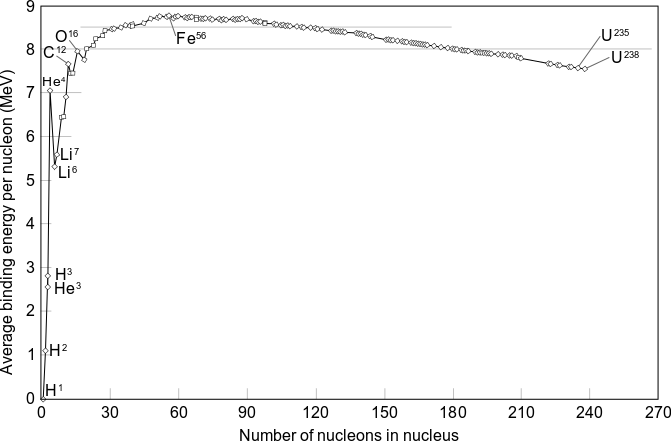
\includegraphics[width=0.75\linewidth]{Kap2/Figures/Binding_energy_curve_-_common_isotopes.png}
    \caption{This figure shows the binding energy per nucleon as a function of the number of nucleons. Source : \cite{BEPN_figure}}
    \label{fig:BE_energy_per_nucleon}
\end{figure}

Processes that result in nuclei with more binding energy per nucleon convert mass into energy \cite{Stacey_2010}. There are two possible processes in which this may happen: fission and fusion reactions. Fusion reactions happen when two light nuclei combine and form a heavier nucleus \cite{Lewis_2014}. On the contrary, fission occurs when a heavier nucleus splits to form lighter nuclei \cite{Stacey_2010}. Fission is the process on which nuclear reactors are based.

\subsection{Liquid-Drop Model}
The liquid-drop model, one of the first nuclear models, was proposed by Bohr in 1935. It is based on the short range of nuclear forces as well as the additivity of volumes and binding energies. The basic idea is that nucleons interact strongly with their neighbours, similar to how molecules interact in a drop of water \cite{Spiro}.

Based on this model, in 1935 Bethe and Weizs\"{a}cker made an excellent parametrization of the binding energies of nuclei in their ground state. This formula extends the idea of the liquid-drop model to incorporate two new ingredients, related to quantum properties of the nuclear mater. The first one is the asymmetric energy which tends to stabilize nuclei with equal number of protons and neutrons. The other is the pairing energy which favors paired fermions \cite{Spiro}. The formula is composed by five therms:

\begin{itemize}
    \item The first parameter in the formula is related to the volume ($a_{v} = 15.753 MeV$). This term reflects the nearest neighbor interactions and leads to a constant binding energy per nucleon.
    \item The term $a_{s}$ lowers the binding energy and is related to the surface of the nucleus. While internal nucleus feel isotropic interactions, nucleus on the surface feel forces coming only from the inside. Since superficial area of a sphere is $4\pi R^2$ and $R \sim A^{2/3}$, this therm is proportional to $A^{2/3}$.
    \item $a_{c}$ is related to the Coulomb repulsion of protons therefore lowers binding energy of the nucleus. Coulomb potential is proportional to $Q^2/R$ thus $a_{c} \sim Z^2/A^{1/3}$.
    \item While $a_{c}$ favors neutron excess over protons, the term $a_{a}$ favors symmetry between protons and neutrons related to the isospin.
    \item Finally, $\delta(A)$ is a quantum pairing term.
\end{itemize}

The Bethe-Weizs\"{a}cker's formula is:\cite{Spiro}

\begin{flalign}
    && B(A,Z) = a_{v}A - a_{s}A^{2/3} - a_{c} \frac{Z^2}{A^{1/3}} - a_{a} \frac{(N-Z)^2}{A} + \delta(A) &&
    \label{eq:binding_energy_ldm}
\end{flalign}

Since this is a empirical formula each parameter $a_{i}$ has to be fitted to the data. This fitting process results in the following values:

\begin{itemize}
    \item $a_{v} = 15.753 MeV$
    \item $a_{s} = 17.804 MeV$
    \item $a_{c} = 0.7103 MeV$
    \item $a_{a} = 23.69 MeV$
    \item $\delta(A) =
        \begin{cases} 
        33.6A^{-3/4} & \text{if } N \text{ and } Z \text{ are even} \\
        -33.6A^{-3/4} & \text{if } N \text{ and } Z \text{ are odd} \\
        0 & \text{if } A = N + Z \text{ is odd}
        \end{cases}$
\end{itemize}

\subsection{Instability of Isotopes}

Induced fission occurs when a probe transfers energy into a nucleus, leaving it in an excited state, which may then split into two fragments of similar size. There are various kinds of probe, but for induced fission reactions, neutrons are the most effective because they do not have an electric charge. Therefore, they do not experience Coulomb repulsion, allowing them to penetrate deeper into the nucleus, bringing energy and causing a rearrangement in the shell structure of the nucleus.\cite{Notas_sanabricas}

For instance suppose and spherical nucleus with:

\begin{flalign*}
    && V = \frac{4}{3} \pi R^3 &&\\
    && S = 4\pi R^2 &&
\end{flalign*}

We will explore the effects of a small deformation like an prolate spheroid. Since nuclear mater is incompressible, the volume will not change, at least to first order. Consider a small deformation, $\epsilon << 1$:

\begin{flalign*}
    && a = R(1+\epsilon) ;b = R(1+\epsilon)^{-1/2} &&\\
    && V = \frac{4}{3} \pi ab^2 = \frac{4}{3} \pi R^3 && 
\end{flalign*}

With these definitions, the volume remains constant, but the surface area increases. Using a Taylor series expansion for small $\epsilon$, we have:

\begin{flalign*}
    && \frac{a}{b} = 1 + \frac{3}{2} \epsilon + \frac{3}{8} \epsilon^2 + \dotsb &&
\end{flalign*}

Also,

\begin{flalign*}
    && \left(\frac{b}{a}\right)^2 = 1 - 3 \epsilon + 6 \epsilon^2 - 10 \epsilon^3 + \dotsb &&
\end{flalign*}

Given $\frac{\arcsin \epsilon}{\epsilon} = 1 + \frac{1}{2} \epsilon - \frac{13}{40} \epsilon^2 + \dotsb$, we get:

\begin{flalign*}
    && \left(\frac{b}{a}\right)^2 \left(\frac{\arcsin \epsilon}{\epsilon}\right) = 2\left(1 + \epsilon + \frac{2}{3} \epsilon^2 + \dotsb\right) &&
\end{flalign*}

Substituting into the surface area $S$:

\begin{flalign}
    && S = 4\pi R^2 \left(1 + \frac{2}{5} \epsilon + \dotsb\right) &&
    \label{eq:S_binding_deformed}
\end{flalign}

Finally, considering the average distance between nucleons inside the deformed nucleus:

\begin{flalign}
    && \Bar{R} &= R \left(1 + \frac{1}{5} \epsilon^2 + \dotsb\right) \nonumber && \\
    && \Bar{R}^{-1} &= R^{-1} \left(1 - \frac{1}{5} \epsilon^2 + \dotsb\right) &&
    \label{eq:R_binding_deformed}
\end{flalign}

Knowing how $\Bar{R}$ and S change in the nucleus with the small deformation \textbf{Eq.}(\ref{eq:R_binding_deformed})  and \textbf{Eq.}(\ref{eq:S_binding_deformed}) respectively, we can evaluate the binding energy \textbf{Eq.}(\ref{eq:binding_energy_ldm}) and see how it changes. The Coulomb and the surface terms are the ones that change. The following analysis will detail these changes:

\begin{flalign*}
    && \Delta E = B(\epsilon) - B(0) &&\\
    && \Delta E = \left(-\frac{2}{5}a_{s}A^{2/3} +\frac{1}{5} a_{c} z (z-1) A^{-1/3} \right) \epsilon^2 &&
\end{flalign*}

If $\Delta E > 0$, then $B(\epsilon) > Bb(\epsilon = 0)$. This means that the deformed nucleus is lighter that the spherical one, resulting in an tendency towards stretching in the nucleus, which leads to fission \cite{Krane}. We will focus on the conditions that lead to $\Delta E > 0$:

\begin{flalign*}
    && -\frac{2}{5}a_{s}A^{2/3} +\frac{1}{5} a_{c} z (z-1) A^{-1/3} > 0 &&\\
    && \frac{1}{5} a_{c} z (z-1) A^{-1/3} > \frac{2}{5}a_{s}A^{2/3} &&\\
    && \left( z \gtrsim 90 \right) \rightarrow z(z-1) \approx z^2 &&\\
    && a_{c} Z^2 > 2 a_{s} A && \\
    && Z^2/A > \frac{2 a_{s}}{a_{c}} &&
\end{flalign*}

The right side of the expression can be approximated $\frac{2 a_{s}}{a_{c}} \approx 47$ which leave us we the condition \cite{Krane}:

\begin{flalign}
    && \frac{Z^2}{A} > 47. && 
    \label{eq:inestability}
\end{flalign}

A nucleus with this property is completely unstable to fission. When discussing about nuclear reactors, we want isotopes that are prone to fission, but this probability should not be too high because spontaneous fission would dominate the reaction, reducing the efficiency of the reactor \cite{Notas_sanabricas}. Nuclei with $Z>90$ and $A>230$ undergo fission relatively easily, either through induced or spontaneous processes.\cite{Lewis_2014}

\subsection{Valley of Instability}

The presence of Coulomb and asymmetric terms in the binding energy \textbf{Eq.}(\ref{eq:binding_energy_ldm}) implies the existence of a maximum in the binding energy for a given \( A \), as a function of \( Z \) \cite{Spiro}. To find this relation, we set \(\partial B/\partial Z = 0\), as shown in the following expression:

\begin{flalign*}
    && \frac{\partial B}{\partial Z}\bigg|_{A=\text{const}} = -2a_{c} \frac{Z_{\text{min}}}{A^{1/3}} + 2 a_{a} \frac{(N-Z_{\text{min}})}{A} &&
\end{flalign*}
Setting this expression to zero and replacing \(N = A-Z\), we get:
\begin{flalign*}
    && 0 = -2a_{c} \frac{Z_{\text{min}}}{A^{1/3}} + 2 a_{a} \frac{(A-2Z_{\text{min}})}{A} && \\
    && 0 = - a_{c} \frac{Z_{\text{min}}}{A^{1/3}} + a_{a} - 2\frac{Z_{\text{min}}}{A} && \\
    && Z_{\text{min}} = \frac{A}{2+a_{c}A^{2/3}/(2a_{a})} &&
\end{flalign*}

This expression can be approximated by \(N = Z = A/2\) and \(a_{c}/a_{a} \approx 0.0075\) \cite{Spiro}. This leaves us with the expression:

\begin{flalign}
    && Z_{\text{min}} \approx \frac{A}{2} \, \frac{1}{1+0.0075 \, A^{2/3}} &&
    \label{eq:stability_valley}
\end{flalign}

The \textbf{Eq.}(\ref{eq:stability_valley}) tells us which is the most stable isotope for a given \( A \). This information will be helpful later in the document when we discuss the requirement of stable isotopes for the reactor fuel.



\section{Nuclear Fission}
A first approximation to study the probability of a nuclear fission, one can suppose that the fission fragments live within the nucleus and fission takes place when one of them surpasses the Coulomb barrier \cite{Notas_sanabricas}.

For instance, consider the fission reaction of a nucleus, specifically $\prescript{235}{}{U}$ undergoing an induced fission reaction. We will delve into this type of fission later in the document. This reaction results in many products such as neutrons, fission fragments and radiation, as shown in \textbf{Fig} (\ref{fig:fission_react}). Each of these products plays its role in a nuclear reactor.

\begin{figure}[h]
    \centering
    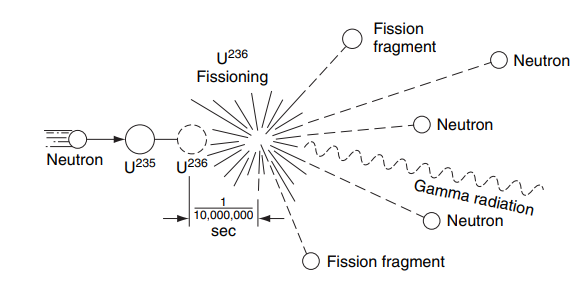
\includegraphics[width=0.75\linewidth]{Kap2/Figures/fission_reaction_stacey.png}
    \caption{Detailed Schematic of a Nuclear Fission Reaction. Source: \cite{Stacey_2010}.}
    \label{fig:fission_react}
\end{figure}

Subsequently, suppose that the nucleus splits in two similar fragments, $\prescript{119}{46}{Pd}$. To compute the energy liberated in the reaction we just need to compute the difference in binding energy between $\prescript{238}{}{U}$ and $2\times\prescript{119}{}{Pd}$, which is equal to 214 MeV.

To continue, we compute the Coulomb barrier, knowing that $R = R_{1} + R_{2}$,  $R_{2} = R_{1}$ and $R_1 = R_{0} (119)^{1/3} = 6\, \text{fm}$:

\begin{flalign*}
    && V = \frac{1}{4\pi \epsilon_{0}} \frac{Z_{1}Z_{2}e^2}{R} &&\\
    && R = 12\, \text{fm} &&\\
    && Z_1 = Z_2 = 46 &&\\
    && V = 253\, \text{MeV} &&
\end{flalign*}    


The excitation energy of the fragments inside $\prescript{238}{}{U}$ is 214 MeV and the height of the Coulomb barrier is 253 MeV. This values are not that different, which  makes the probability non-zero for one of the fragments escaping the nucleus because of quantum tunneling. This calculation is a mere sketch  of what a real calculation needs to consider. For example, if we choose the two fragments to be $\prescript{79}{30}{Zn}$ and $\prescript{159}{62}{Sm}$ the Coulomb barrier will be reduced to 221. In more sophisticated version of these calculations, two new parameters will be added:

\begin{itemize}
    \item Fission barrier 
    \item activation energy
\end{itemize}

These more sophisticated calculation are based on the liquid-drop model and give us an idea of the activation energy, the energy required for a nucleus to surpass the fission barrier and fission \cite{Krane}.

When a neutron is absorbed into a heavy nucleus resulting in a compound nucleus, the binding energy per nucleon decreases. For some nuclei, such as $\prescript{233}{92}{U}$, $\prescript{235}{92}{U}$, $\prescript{239}{92}{Pu}$, this decrease is so significant that the compound nucleus will undergo fission with high probability, even if the neutron has very low energy \cite{Stacey_2010}. A compound nucleus is an excited nucleus which decays via multiple paths, depending on the isotope.

\subsection{Fission Products}
Fission is an asymmetric process, this means the two resulting fragments have different masses. However, the probability that the two fragments have the same mass is close to zero, which is not well understand \cite{Notas_sanabricas}. 

\begin{figure}[h]
    \centering
    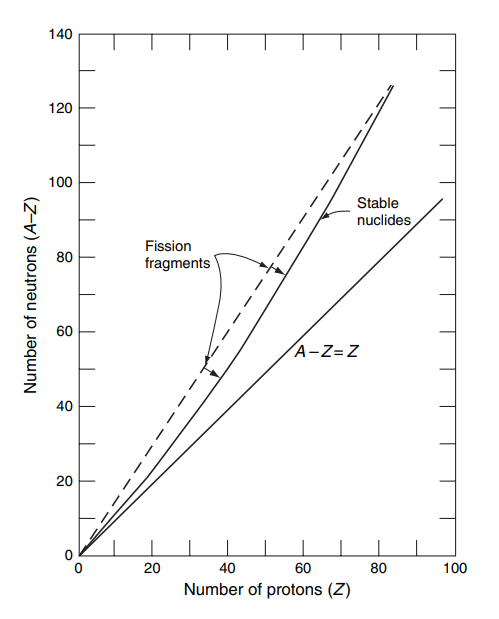
\includegraphics[width=0.5\linewidth]{Kap2/Figures/stability_curve.png}
    \caption{Graph illustrating the relationship between the number of neutrons and the number of protons in nuclei. Source: \cite{Lewis_2014}}
    \label{fig:Stability_curve}
\end{figure}

Fission fragments are unstable because they neutron excess \cite{Lewis_2014}. When a nucleus undergoes fission, it not only produces fragments but also emits neutrons, known as prompt neutrons. This emission changes the proton-to-neutron ratio of the fragments. Nonetheless, these fragments still lie about the stability curve in \textbf{Fig} (\ref{fig:Stability_curve}). Some of these nuclei, less than $1\%$, decay by delayed-neutron emission, most of the fragments decay via beta emission or gamma rays. For example:

\begin{flalign*}
    && n + \prescript{235}{92}{U} &\rightarrow \prescript{140}{54}{Xe} + \prescript{94}{38}{Sr} + 2n + 200MeV &&
\end{flalign*}

$\prescript{140}{54}{Xe}$ follows the chain of reactions:

\begin{flalign*}
    && \prescript{140}{54}{Xe} \xrightarrow{\beta} \prescript{140}{55}{Cs} \xrightarrow{\beta} \prescript{140}{56}{Ba} \xrightarrow{\beta} \prescript{140}{57}{La} \xrightarrow{\beta} \prescript{140}{58}{Ce} &&
\end{flalign*}

This process shows only one of the 40 possible pairs that results from fission \cite{Lewis_2014}. These fragments are highly radioactive and, in some cases, they can produced delayed neutron. Prompt and delayed neutrons play and fundamental role in the dynamics of a nuclear reactor.

\subsection{Fission Cross Sections}
Next we are going to focus on $\sigma$ known as the nuclear reaction cross-section, which is a value that quantifies the probability of a nuclear reaction occurring \cite{Stacey_2010}. This parameter is expressed in terms of the number of neutrons traveling with speed $v$ a distance $dx$ in a material with N nuclei per unit volume

\begin{flalign}
    && \sigma := \frac{\text{reaction rate}}{nvNdx} &&
\end{flalign}

$\sigma$ has units of area, consistent with the idea that $\sigma$ is an effective area of interaction. That is why is called `cross-section'. Typically, this parameter is measured in Barns. $1\text{barn} = 10^{-24} cm$ \cite{Stacey_2010}.

 The fission cross section ($\sigma_{f}$), represents the probability that the interaction of a neutron and a nucleus will result in fission \cite{Stacey_2010}. The probability peaks when the energy delivered to the nucleus, matches the energy difference between an excited state and the ground state of the compound nucleus. This phenomenon is known as resonances \cite{Stacey_2010}. 

$\prescript{238}{}{U}$ fissions only by \textit{fast neutrons} which are neutrons of high energy (energies around MeV). However, this cross section is small compared to others \cite{Notas_sanabricas}. On the other hand, $\prescript{235}{}{U}$ and $\prescript{239}{}{Pu}$ undergo fission with neutrons across all energy spectra present in a nuclear reactor \cite{Notas_sanabricas}, as shown in \textbf{Fig} (\ref{fig:Cross_section_fission}), including its resonances, which corresponds to the peaks in the graph.

\begin{figure}
    \centering
    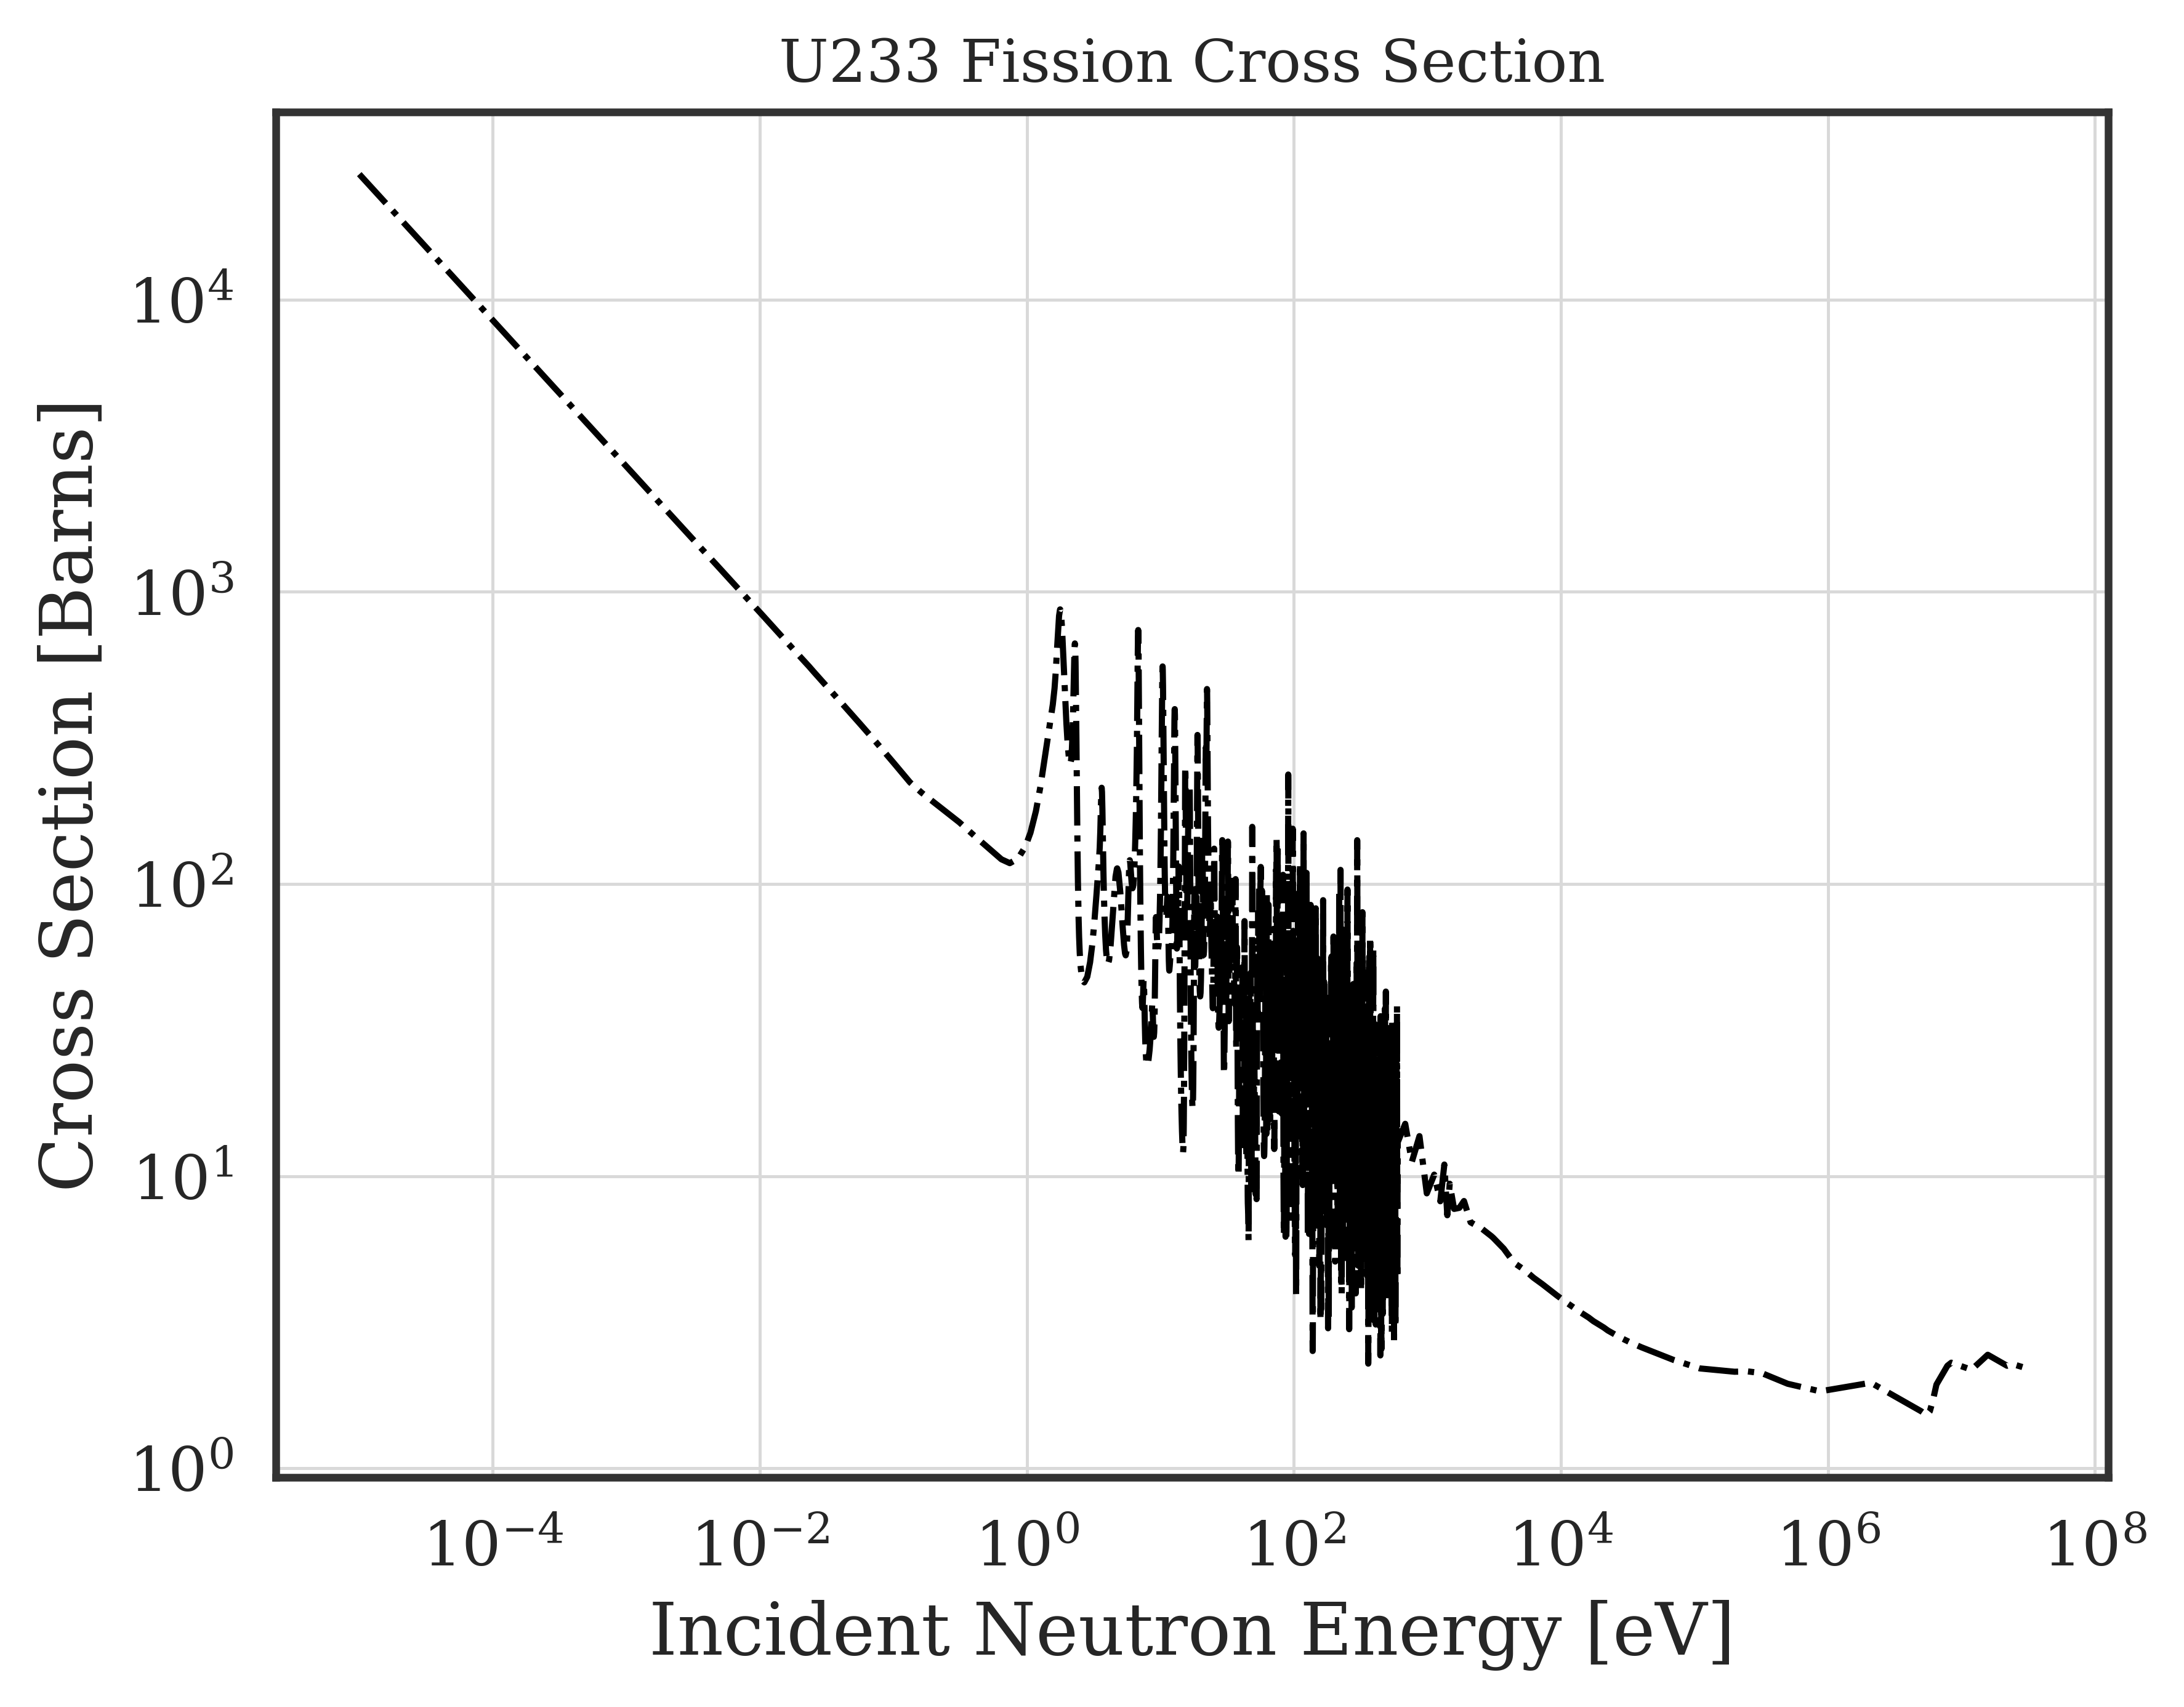
\includegraphics[width=0.75\linewidth]{Kap2/Figures/U233_Cross_Section.png}
    \caption{Fission cross section of $\prescript{233}{}{U}$. Data retrieved from \cite{NNDC}}
    \label{fig:Cross_section_fission}
\end{figure}

\section{Abundances of Isotopes}
\label{sec:possible_fuels}

We already explored the instability of isotopes. Relation \textbf{Eq.}(\ref{eq:inestability}) give us an idea of how prone is a nucleus to fission. For instance, if we compute this parameter for the following nuclei, we get:

\begin{align*}
    \prescript{208}{82}{Pb} \rightarrow 32.33\\
    \prescript{232}{90}{Th} \rightarrow 34.91\\
    \prescript{238}{92}{U} \rightarrow  35.56\\
    \prescript{235}{92}{U} \rightarrow 36.02\\
    \prescript{233}{92}{U} \rightarrow 36.33\\
    \prescript{239}{94}{Pu} \rightarrow 36.97\\
    \prescript{252}{94}{Cf} \rightarrow 38.11
\end{align*}

All isotopes can undergo fission if they are hit with enough energy. In nuclear physics, probes usually have kinetic energies around MeV. Lead (Pb) is a very stable isotope. Isotopes, including Thorium-232 ($\prescript{232}{}{Th}$) and Uranium-238 ($\prescript{238}{}{U}$), have a non-zero probability of fission, yet their cross-sections are small. In contrast, isotopes, such as $\prescript{235}{}{U}$, $\prescript{233}{}{U}$ and $\prescript{239}{}{Pu}$, are more prone to fission. Nuclei over Plutonium (Pu) can undergo spontaneous fission. This condition worsens for isotopes with $Z^2/A \geq 39$ which have infinitesimally small mean life \cite{Notas_sanabricas}. Bringing this in mind, we can estimate some ranges for the stability of isotopes:
\begin{center}
\begin{align*}
    Z^2/A < 35 &\rightarrow \text{Too stable}\\
    Z^2/A \sim 35 &\rightarrow \text{Fissile but not that much}\\
    Z^2/A \sim 36 &\rightarrow \text{Prone to fission}\\
    Z^2/A \sim 38 &\rightarrow \text{Spontaneous fission}\\
    Z^2/A  \gtrsim 39 &\rightarrow \text{Too unstable} \\
    Z^2/A > 47 &\rightarrow \text{Not possible}
\end{align*}
\end{center}

Besides, we have to look for isotopes that are close to the bottom of the valley of stability \textbf{Eq.} (\ref{eq:stability_valley}). Those far away from the valley will decay via $\beta^{+/-}$, $\alpha$, neutron or proton evaporation \cite{Notas_sanabricas}. This leaves us with three possible isotopes:

\begin{center}
\begin{align*}
    \prescript{233}{}{U} &\rightarrow \tau = 160000 \, \text{years}\\
    \prescript{235}{}{U} &\rightarrow \tau = 700  \, \text{million years}\\
    \prescript{239}{}{Pu} &\rightarrow \tau = 24000  \, \text{years}
\end{align*}
\end{center}

For an approximation of how much of each material is available on Earth, we are going to compare their mean life with the lifespan of Earth which is around $4.54$ billion years. $\prescript{239}{}{Pu}, \tau = 24000 \, \text{years}$ This means it has passed $187000$ mean lifespans since the creation of Earth, which indicates there is no plutonium left on earth. Something similar happens for $\prescript{233}{}{U}$. Quite the contrary is the case of $\prescript{235}{}{U}$ which has a mean life comparable to earth's age, which means there is $\prescript{235}{}{U}$ on the planet but not that much.

The uranium available on Earth is known as `natural uranium' ($\prescript{Nat}{}{U}$). Its composition is : 

\begin{equation*}
    \begin{cases}
        \prescript{238}{}{U} &\rightarrow 99.274\%\\
        \prescript{235}{}{U} &\rightarrow 0.720\%\\
        \prescript{234}{}{U} &\rightarrow 0.005\%
    \end{cases}
\end{equation*}

These isotopes are the ones that could be used as initial nuclear fuel for a nuclear reactor \cite{Notas_sanabricas}.

\subsection{Notation}

Latter on this document an special notation will be used to indicate the isotopes discussed here. The reader may notice the following pattern:

\begin{align*}
    Th \rightarrow Z=90\\
    Pu \rightarrow Z=94\\
    Z \in [90,94]
\end{align*}

As well as :

\begin{align*}
    \prescript{232}{}{Th} \rightarrow A = 232\\
    \prescript{239}{}{Pu} \rightarrow A = 239\\
    A \in [232, 239]
\end{align*}

So we can think that we have the `general case':

\begin{equation*}
    \prescript{23b}{9a}{X} \rightarrow \begin{cases}
        a = 0,1,2,3,4\\
        b = 2,3,4,5,6,7,8,9
    \end{cases}
\end{equation*}

So we can use this two numbers to refer to a certain isotope. For example:

\begin{align*}
    \prescript{232}{90}{Th} &\rightarrow 02\\
    \prescript{235}{92}{U} &\rightarrow 25\\
    \prescript{238}{92}{U} &\rightarrow 28
\end{align*}

\subsection{Fissionable and Fertile Material}

Having introduced the fuel of a nuclear reactor, now we have to distinguish between two sub classes of fissionable material. Firstly, we have fissile nuclei which are the ones that undergo fission when they are irradiated by neutrons of some energy. For example $\prescript{235}{}{U}$ is fissile. Secondly, we have fertile material which can undergo fission only by high energy neutrons. However, fertile materials can become fissile if they captures neutrons, trans-mutating via $\beta$ decays or capturing neutrons again. This is the case of Thorium-232 ($\prescript{232}{}{Th}$) and Uranium-238 ($\prescript{238}{}{U}$).

\begin{flalign*}
    && n + \prescript{238}{92}{U} \rightarrow \prescript{239}{92}{U}^{*} \xrightarrow{\beta^{-}} \prescript{239}{93}{Np} \xrightarrow{\beta^{-}} \prescript{239}{94}{Pu} &&
\end{flalign*}

\begin{flalign*}
    && n + \prescript{232}{90}{Th} \rightarrow \prescript{233}{90}{Th}^{*} \xrightarrow{\beta^{-}} \prescript{233}{91}{Pa} \xrightarrow{\beta^{-}} \prescript{233}{92}{U} &&
\end{flalign*}

The crust of Earth has at least three times more Thorium-232 than Uranium \cite{IAEA2005}. Using this material to breed $\prescript{233}{}{U}$ is the idea behind a Thorium fuel cycle. However, a breeding chain reaction is more difficult to sustain than a fission chain reaction \cite{Notas_sanabricas}.

\section{Neutron Interactions}

In order to produce energy, a nuclear reactor must sustain an equilibrium between the neutrons generated within the core and the neutrons lost\cite{Lamarsh_Baratta_2009}.To achieve this, a nuclear reactor must sustain an induced fission chain reaction. In this process, neutrons, produced by fission, induced new fissions in other fissile nuclei \cite{Lamarsh_Baratta_2009}. These new fissions produce more neutrons, which induce further reactions, repeating the process. \textbf{Fig} (\ref{fig:chain_reaction}) illustrates this process.

In each fission of $\prescript{235}{}{U}$, an average of 2.4 neutrons are produced \cite{Lewis_2014}. We have already seen that around $200$ MeV of energy is liberated after the fission of $\prescript{235}{}{U}$. Nonetheless, this energy is released as kinetic energy of the fission fragments (FF) and is eventually dissipated as heat.

\begin{figure}[h]
    \centering
    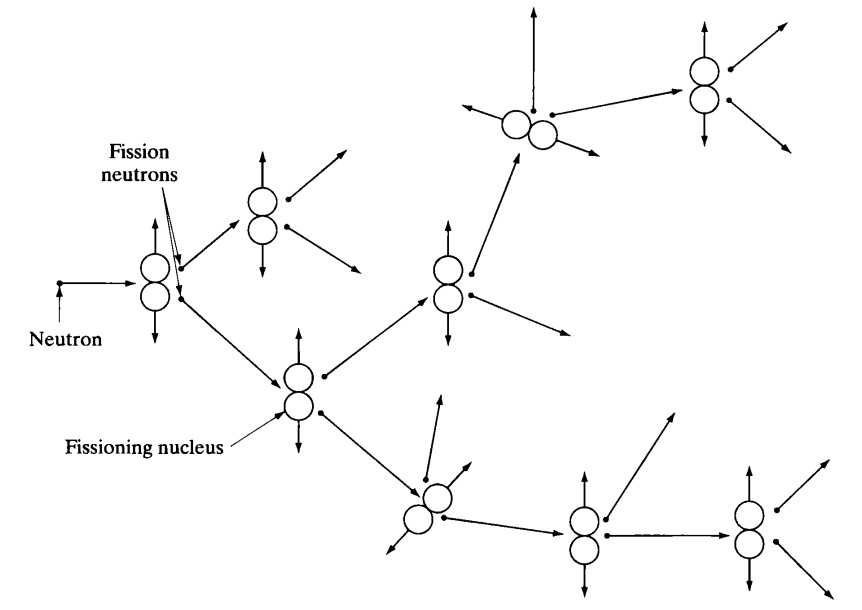
\includegraphics[width=0.75\linewidth]{Kap2/Figures/Chian_reaction.png}
    \caption{Fission reaction chain schematic. Source: \cite{Lewis_2014}}
    \label{fig:chain_reaction}
\end{figure}

\subsection{Neutron Multiplication}

The reaction represented in \textbf{Fig} (\ref{fig:chain_reaction}) can be described in terms of a parameter known as `multiplication factor', denoted as \(k\) \cite{Lewis_2014}. The factor is defined as the number of neutrons produced in one generation divided by the number of neutrons produced in the preceding generation.

\begin{flalign}
    && k := \frac{\text{Number of fission's neutrons produced in one generation}}{\text{Number of fission's neutrons produced in the preceding generation}} &&
    \label{eq:def_multiplicative_factor}
\end{flalign}


In addition, if we want to estimate the number of neutrons produced in one generation, we need to use \(l\), which is the lifespan of a neutron inside the reactor \cite{Lewis_2014}. This is the time between the production and the absorption of neutrons. Suppose that there are $n_0$ neutrons at $t=0$, then, we can use the following formula to compute the number of neutrons of the \(ith\) generation:

\begin{flalign}
    && n(t) = n_0 k^{t/l} &&
\end{flalign}

There are three possibilities for the values of \(k\):

\begin{center}
$
    k= \begin{cases}
        k > 1 : \text{``Supercritical''. Neutrons increases exponentially.}\\
        k = 1 : \text{``critical''. The number of neutrons remains constant.}\\
        k < 1 : \text{``Subcritical''. The number of neutrons decreases.}
    \end{cases}
$
\end{center}

\subsection{Heat Produced by the Fuel}

Around \(8\%\) of the 200 MeV of the energy produced by fission corresponds to the gamma rays associated with the beta decays of fission products \cite{Lewis_2014}. Therefore, after a shutdown, a reactor that has been operating a for a time will keep radiating a significant amount of heat \cite{Lewis_2014}. The heat produced after shutdown due to beta and gamma decays could be computed using the Wigner-Way formula.

\begin{flalign}
    && P_{d}(t) = 0.0622 P_{0}[t^{-0.2}+(t_{0}+t)^{-0.2}] &&
    \label{eq:heat_decays}
\end{flalign}

Where \(P_{d}(t)\) is the power generated at time \(t\), \(P_{0}\) is the power of the reactor before the shutdown and \(t_{0}\) is the time of power operation before the shutdown. Due to the decay heat produced after the shutdown, the reactor must be refrigerated to prevent overheating for a considerable period of time \cite{Lewis_2014}.

\section{Microscopic and Macroscopic Cross Sections}

After the previous discussion on nuclear fuel, we want to determine how neutrons interact with the material inside the reactor. To achieve this, let us consider a beam of neutrons traveling in the \(+x\) direction. The intensity of the beam is given by $I = n'''v$, where $n'''$ \footnote{In this notation, quantities marked with triple primes (\('''\)) represent volumetric densities, double primes (\(''\)) indicate surface densities, and single primes (\('\)) denote linear densities.} is the volumetric neutron's density and \(v\) is the velocity at which all of the neutrons are traveling \cite{Lewis_2014}.

We assume that a neutron that collides with a nucleus is either absorbed or scattered into a different direction, reducing the number of neutrons traveling in the same direction \cite{Lewis_2014}. This causes a decline in the intensity of the beam.

Let \(I(x)\) be the intensity of the beam after penetrating a distant x in the material. Then, if the beam travels an additional infinitesimal distance \(dx\), some neutrons will be removed. This removal is proportional to the number of nucleus in this region denoted as \(N\) and the cross-section, $\sigma$ \cite{Lewis_2014}. Therefore, we have:

\begin{flalign*}
    && I(x + dx) = (1 - N\sigma dx)I(x) &&
\end{flalign*}
If $I(0) = I_{0}$ and applying the derivative:

\begin{flalign*}
    && \frac{d}{dx} I(x) = -N\sigma I(x) &&
\end{flalign*}

Solving the differential equation an integrating from 0 to x:

\begin{flalign}
    && I(x) = I_{0}e^{-N\sigma x} &&
    \label{eq:mics_collided_flux}
\end{flalign}

\subsection{Macroscopic Cross Section}

After this result, we want to introduce the macroscopic cross section, defined as:

\begin{flalign}
    && \Sigma := N\sigma &&
    \label{eq:def_macs}
\end{flalign}

Where $\sigma$ refers to the microscopic cross section, measured in $cm^2/nucleus$, and N is still the volumetric nuclei density, measured in $nuclei/cm^3$. Then, the macroscopic cross section must have units of $cm^-1$.

Replacing $N\sigma$ in \textbf{Eq.}(\ref{eq:mics_collided_flux}) with $\Sigma$, we obtain a macroscopic version of the flux. We can interpret this collided flux as a probabilistic distribution indicating the likelihood of a neutron reaching a depth \(x\) into a material without colliding \cite{Lewis_2014}.

\begin{flalign*}
   && I(x) = I_{0}e^{-\Sigma x} &&
\end{flalign*}

Dividing \(I(x)\) by \(I_{0}\), we obtain the fraction of neutrons that have reached a distance \(x\) without colliding. Interpreting \(\frac{dI}{dx} = - \Sigma I(x)\) as the probability of a neutron having its first collision in the next \(dx\), we have:


\begin{flalign*}
   && p(x)dx = (\Sigma dx) (\frac{I(x)}{I_{0}}) = \Sigma e^{-\Sigma x} dx &&
\end{flalign*}

We can compute the mean free path \(\lambda\), the mean distance traveled by a neutron between collisions, as \cite{Lewis_2014}:

\begin{flalign*}
    && \lambda = \int_{0}^{\infty}xp(x)dx = \int_{0}^{\infty}x\Sigma e^{-\Sigma x}dx = \frac{1}{\Sigma} &&
\end{flalign*}

\section{Nuclei Density (N)}

The Avogadro's number is the total of molecules in a mole of a substance, $N_0 = 0.6023 \cdot 10^24$ \cite{Lewis_2014}. In order to compute the  density of the molecule of a substance, we have to divide $N_0$ by the molecular wight \(A\) and, finally, multiply it by the density of the substance \(\rho\) \cite{Lewis_2014}:

\begin{equation*}
    N = \rho N_{0}/A
\end{equation*}

Replacing this in \textbf{Eq.}(\ref{eq:def_macs}) we have:

\begin{equation*}
    \Sigma = \frac{\rho N_{0}}{A}\sigma
\end{equation*}

Now if we apply this formula to an chemical element we have to consider that this element, in reality, exist in nature as a mixture of isotopes. To adjust the formula to this case we denote $N^{i}/N$ as the atomic fraction of the isotope with $A_i$ atomic weight, Thus we define the atomic weight of the mixture as \cite{Lewis_2014}:

\begin{equation*}
    A = \sum_{i} (N^{i}/N) A_{i} ,
\end{equation*}

where $N = \sum_{i}N^{i}$. Applying this to get the macroscopic cross section we get:

\begin{equation}
    \Sigma = \frac{\rho N_{0}}{A} \sum_{i}\frac{N^{i}}{N} \sigma^{i}
    \label{eq:chemical_mcs}
\end{equation}

Where $\sigma^{i}$ is the microscopic cross section of the \(ith\) isotope.

In many cases material are combined using volume fractions. Once again, we want to make adjustment to our equation to consider this situation. Let $V_{i}/V$ the volume fraction where $V = \sum_{i}V_{i}$, the cross section of the mixture is \cite{Lewis_2014}:

\begin{equation}
    \Sigma = \sum_{i}(V_{i}/V)N_{i}\sigma^{i}
    \label{eq:mcs_chemical_vf}
\end{equation}.

To compute each of the nuclei number density we make use of the density of the \(ith\) nuclei $\rho_{i}$ and its atomic weight $A_{i}$

\begin{equation*}
    N_{i} = \rho_{i}N_{0}/A_{i}
\end{equation*}

The expression in \textbf{Eq.}(\ref{eq:mcs_chemical_vf}) can be re written in terms of the macroscopic cross section of its components.

\begin{equation*}
    \Sigma = \sum_{i}(V_{i}/V)\Sigma^{i}
\end{equation*}

Where $\Sigma^{i} = N_{i}\sigma^{i}$. This expression can also be written in terms of mass fractions. Applying the same idea as before we get:

\begin{equation*}
    \sigma = \sum_{i}(M_{i}/M) \frac{\rho N_{0}}{A_{i}} \sigma^{i}
\end{equation*}

Where $M_i/M = \rho_{i}V_{i}/(\rho_{i}V)$ is the mass fraction, $M = \sum_{i}M_{i}$ and $\rho = M/V$.

\subsection{Enriched Uranium}

We have already mentioned that in nature uranium is found as a mixture of two main isotopes: $99.3\%$ of $\prescript{238}{}{U}$ and $0.7\%$ of $\prescript{235}{}{U}$. However, in a nuclear reactor, enriched uranium is needed which is uranium where the mass fraction of $\prescript{235}{}{U}$ has been increased. We denote the enrichment as \cite{Lewis_2014}:

\begin{flalign}
    && \Tilde{e_a} = \frac{N^{25}}{(N^{25}+N^{28})} &&
    \label{eq:Atomic_enr}
\end{flalign}

This expression is known as the atomic enrichment, and from the definition, we can deduced that $1-\Tilde{e_{a}} = N^{28}/(N^{28}+N^{25})$ is the Uranium-238 fraction. We can compute the macroscopic cross section using the enrichment as follows \cite{Lewis_2014}:

\begin{flalign*}
   && \Sigma^{U} = \frac{\rho_{U}N_{0}}{\Tilde{e_{a}}235 + (1-\Tilde{e_{a}})238}[\Tilde{e_{a}}\sigma^{25}+(1-\Tilde{e_{a}})\sigma^{28}] &&   
\end{flalign*} 

Another definition way to defined the enrichment is using the masses:

\begin{flalign*}
    && \Tilde{e_{w}} = \frac{M^{25}}{(M^{28}+M^{25})} &&
\end{flalign*}

We can also get the mass fraction for $\prescript{238}{}{U}$ based on the enrichment by $1-\Tilde{e_{w}} = \frac{M^{28}}{(M^{25}+M^{28})}$. Using this definition to compute the macroscopic cross section:

\begin{flalign*}
    && \Sigma^{U} = \rho N_{0} \left[ \frac{1}{235}\Tilde{e_{w}}\sigma^{25} + \frac{1}{238}(1-\Tilde{e_{w}})\sigma^{28}\right] && 
\end{flalign*}

There exits a relation between $\Tilde{e_{a}}$ and $\Tilde{e_{w}}$. Using $N^{25} \sim M^{25}/235$ and $N^{28} \sim M^{28}/238$:

\begin{flalign*}
    && \Tilde{e_a} = \frac{\frac{M^{25}}{235}}{(\frac{M^{25}}{235}+\frac{M^{25}}{235})} &&\\
    && \Tilde{e_a} = \frac{\frac{1}{235}\frac{M^{25}}{M}}{(\frac{1}{235}\frac{M^{25}}{M}+\frac{1}{238}\frac{M^{28}}{M})} &&\\
    && \text{Using} \Tilde{e_{w} \sim \frac{M^{25}}{M}} \text{and} 1-\Tilde{e_{w} \sim \frac{M^{28}}{M}} &&\\
    && \Tilde{e_a} = \frac{\frac{238}{235}\Tilde{e_{w}}}{(\frac{238}{235})\Tilde{e_{w}}+(1-\Tilde{e_{w}})} &&
\end{flalign*}

which finally becomes:

\begin{flalign*}
    && \Tilde{e_a} = \frac{1.0128\Tilde{e_{w}}}{1+0.0128\Tilde{e_{w}}} &&
\end{flalign*}

Using the relation for a level $\Tilde{e_{w}} = 0.007$, the atomic enrichment would be $\Tilde{e_{a}} = 0.00709$, and the values gets closer the higher the enrichment. This means that the approximation $\Tilde{e_{w}} \approx \Tilde{e_{a}} \approx \Tilde{e}$ is accurate.

\section{Neutrons Cross Sections}

So far, we have only introduced the probability that a neutron interacts with a nucleus but we have not talked about the processes that could happened afterwards. The cross section introduced before is known as the total cross section an is denoted as $\sigma_{t}$. When a neutron hits a nucleus, it is either scatter or absorbed, this could be considered in our relations as \cite{Lewis_2014}:

\begin{flalign*}
    && \sigma_{f} = \sigma_{s} + \sigma_{a} &&
\end{flalign*}

In the expression $\sigma_{s}$ and $\sigma_{a}$ denotes the scattering and absorption cross sections. With this formulation of the total cross section we can easily compute the probability for given interaction to end in scattering or absorption using the fractions $\sigma_{s}/\sigma_{t}$ and $\sigma_{a}/\sigma_{t}$ respectively.  

However, the scattering cross section is divided further into elastic and inelastic scattering \cite{Lewis_2014}. In the inelastic scattering the neutron give energy to the nucleus leaving it in an excited state. Both kinds of scattering conserve momentum, but only elastic scattering conserve kinetic energy. This arises in the expression:

\begin{flalign*}
    && \sigma_{s} = \sigma_{n} + \sigma_{n'} &&
\end{flalign*}

Where $\sigma_{n'}$ denotes the cross section for the inelastic scattering.
Something similar happens with the absorption scattering. 

\begin{flalign*}
    &&b\sigma_{a} = \sigma_{\gamma} + \sigma_{f} &&
\end{flalign*}

We have two processes, the first one is the formation of a compound nucleus that does not re emit the neutron but eliminates its exited energy via gamma decays, denoted as $\sigma_{\gamma}$. This process is known as capture reaction and the remaining nucleus could be unstable and decay later on \cite{Lewis_2014}. The other process, more interesting for our application, is a fission process $\sigma_{f}$.

We express a particular macroscopic cross section using a sub index $x = s, a, \gamma, f$ which indicates the particular reaction that we are considering.

\begin{flalign*}
    && \Sigma_{x} = N\sigma_{x} &&
\end{flalign*}

\subsection{Neutron Energy Range}

We have talked about cross sections but we have not considered it energy dependence. In this case, their dependence refers to the energy of the neutron. First we have to establish an upper and a lower limit for the neutron's energy distribution.

\begin{itemize}
    \item Thermal neutrons: 0.001eV - 1.0 ev
    \item Intermediate neutrons: 1.0eV - 0.1MeV
    \item Fast neutrons: 0.1MeV - 10MeV
\end{itemize}

Neutron produced in a fission reaction follow a energy distribution. If $\chi$(E) is the energy distribution then a reasonable approximation of the distribution \cite{Lewis_2014}: 

\begin{flalign}
    && \chi(E) = 0.453 \exp{(-1.036E)}\sinh{(\sqrt{2.29}E)} &&
    \label{eq:dist_fission_neutrons}
\end{flalign}

Prompt neutrons suffer multiple collisions before being absorbed. The nuclei with which they collide follow a thermal distribution with \(E_{N} = \frac{3}{2}kT\), where \(T\) is the temperature of the reactor. Therefore, when neutrons collide, they lose energy, passing through an intermediate energy region. Eventually, those neutrons become thermal neutrons, which follow a Maxwell-Boltzmann distribution. These distributions are important because, later in the document, we will see the dependence of cross sections on energy, and this dependence can change the dynamics of the nuclear reactor.




\chapter{The Design of a Nuclear Reactor}
Following our study of cross sections and the interactions between nuclei and neutrons, we will now delve into the properties of the nuclear fuel. This chapter will explore the dependence of cross sections on energy, analyze the distributions of neutrons, and estimate the multiplication factor, \( k \).

To achieve this, we will examine how different materials within the reactor core influence reaction rates and the neutron flux distribution across the energy spectrum.


\section{Nuclear Fuel Properties}

Cross sections of fissile and fertile materials are functions of energy; therefore, many of the processes that occur inside a nuclear reactor are determined by the energy of the neutrons. The dependence on energy of the cross sections extends over a broad range from: \(10\) MeV to \(0.001\) eV. Fertile materials can undergo fission when absorbing neutrons, but only if the transfer energy surpasses a threshold. A fraction of the total neutrons will be absorbed; this fraction is also energy-dependent. This leads to the following expression:

\begin{equation}
    \eta (E) = \frac{\nu \Sigma_{f}(E)}{\Sigma_{a}(E)}
    \label{eq:first_eta_def}
\end{equation}

The expression represents the fraction of neutrons that create new neutrons after being absorbed. $\nu$ is the number of neutrons produced by fission, and $\Sigma_{x}$ represents the cross section of the fission and absorption processes. By definition, $\Sigma$ depends on the nuclei density, so we can cancel out these factors and end up with $\sigma$.

However, nuclear fuel is composed of multiple isotopes, then $\sigma_{x}$ should be adjusted to consider the mixture of isotopes. First, we have to consider the enrichment \textbf{Eq.}(\ref{eq:Atomic_enr}). We are going to label the cross sections as $\sigma_{x}^{y}$, where \(x\) indicates the process considered (\(f\) for fission and \(a\) for absorption), and \(y\) indicates the fissionable material (\(fi\) for fissile and \(fe\) for fertile). All of these considerations lead to the following expression:

\begin{flalign}
   && \eta (E) = \frac{\nu \, \Tilde{e} \, \sigma_{f}^{fi}(E) + \nu \, (1-\Tilde{e}) \, \sigma_{f}^{fe}(E)}{\Tilde{e} \, \sigma_{a}^{fi}(E) + (1-\Tilde{e}) \, \sigma_{a}^{fe}(E)} &&
    \label{eq:eta_def_fi_fe}
\end{flalign}

The changes caused by the level of enrichment are reflected on \textbf{Fig} \ref{fig:Eta_enrichment}.

\begin{figure}
    \centering
    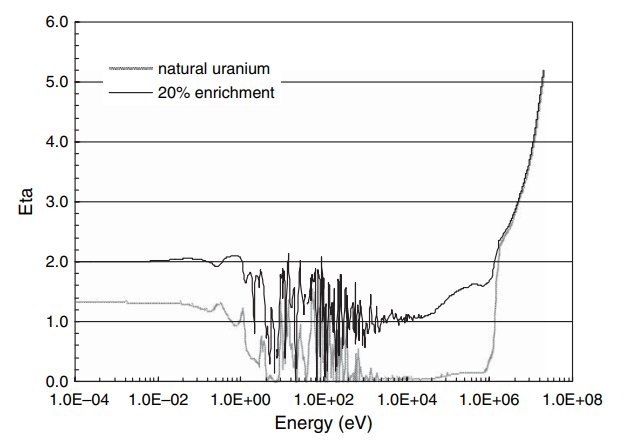
\includegraphics[width=0.75\linewidth]{Kap3/Figures_Kap3/Eta_enrichment.png}
    \caption{Figure showing two plots of $\eta$ as function of energy for uranium fuel at different levels of enrichment. From \textbf{Ref.} \cite{Lewis_2014}}
    \label{fig:Eta_enrichment}
\end{figure}

Nuclear reactors are designed to concentrate in the fast or thermal energy ranges, this is due to the valley in the intermediate energy range. As mentioned before in the document, neutrons lose energy due to elastic scattering, until they reach thermal equilibrium with the medium. There are two types of nuclear reactors, fast and thermal reactors, each one with their own specifications.

In fast reactor design inside the core any kind of material is avoided, different from fuel, so that neutrons experience few scatterings and stay in the fast energy range. Low atomic weight materials are capable to quickly reduce neutrons energy, consequently, they are avoided. This increases the possibility for uranium-238 to absorb neutrons, which depletes the amount neutrons \cite{Lewis_2014}. This makes it impossible for a fast reactor to be fueled with natural uranium \cite{Lewis_2014}; it needs of high enrichment-uranium (HEU) with $\Tilde{e} \gtrsim 10\%$. 

The opposite situation happens for thermal reactors. They need materials, called moderators, to slow-down the neutrons. A thermal nuclear reactor can operate with much lower enrichment \cite{Lewis_2014}. We must examine the properties of moderators to understand their behavior.  

\section{Slow Down Decrement}

To measure the effectiveness of a nucleus to slow neutrons down by elastic scattering, we use the slow down decrement, denoted as $\xi$. It is defined as the mean value of the logarithm of the fraction of energy lost \cite{Lewis_2014}:

\begin{flalign}
    && \xi := \overline{\ln\left(\frac{E}{E}\right)} = \int \ln\left(\frac{E}{E'}\right) p(E \rightarrow E') dE' &&
    \label{eq:def_xi}
\end{flalign}

A long deduction gives us that:
\begin{flalign}
    &&  p(E \rightarrow E') = \frac{1}{(1 - \alpha) E} dE' &&
    \label{eq:dist_energy_scatter}
\end{flalign}

Where $\alpha = \left(\frac{A-1}{A+1}\right)^{2}$, which can be replaced into \textbf{Eq.}(\ref{eq:def_xi}) resulting in:

\begin{flalign}
    && \xi = 1 + \frac{\alpha}{1 - \alpha} \ln \alpha &&
    \label{eq:def_sl_decre}
\end{flalign}

This parameter can be approximated as $\xi \approx \frac{2}{A + 2/3}$. With it, we can estimate the number of collisions necessary to reduce the energy of a neutron from fast neutrons to thermal neutrons. For instance, consider \(E_{1}, E_{2}, \dots, E_{n}\) to be the neutron energies after the \(i\)-th collision, this would be:

\begin{flalign}
    && \ln\left(\frac{E_{0}}{E_{n}}\right) = \ln\left(\frac{E_{0}}{E_{1}}\right) + \ln\left(\frac{E_{1}}{E_{2}}\right) + \dots + \ln\left(\frac{E_{n-1}}{E_{n}}\right) &&
\end{flalign}

Replacing each of the terms for the average logarithmic energy loss \(\xi\), we have:

\begin{flalign}
   && n = \frac{1}{\xi} \ln\left(\frac{E_{0}}{E_{n}}\right) &&
\end{flalign}

Evaluating the expression for hydrogen, we get $n \approx 18$. However, this expression considers only one kind of nucleus. In order to consider the effects of other isotopes, we have to make an average over their \(\xi\), resulting in:

\begin{flalign}
    && \overline{\xi} = \frac{1}{\Sigma_{s}} \sum_{i} \xi_{i} \Sigma_{si} &&
    \label{eq:def_ave_sd_decre}
\end{flalign}

The concept of the slow down decrement is crucial in understanding how neutrons lose energy through collisions. This directly impacts the design and efficiency of neutron moderators, which are essential components in thermal reactors.

\section{Neutron Moderators}

Thermal reactors must reduce the neutrons' energy with as few collisions as possible so that they make the transit to the thermal region without being absorbed in resonance processes \cite{Lewis_2014}. The slowing down decrement is the parameter most suitable for this purpose.

A good moderator must possess additional properties, beyond just a high slowing down decrement. One crucial property is the slowing down power, defined as $\xi \Sigma_s$, where $\Sigma_s$ is the macroscopic scattering cross section. This parameter indicates the effectiveness of a material in slowing down neutrons through scattering interactions. A high slowing down power ensures that neutrons lose energy efficiently during collisions.

Another important parameter is the slowing down ratio, which is the ratio of the material's slowing down power to its thermal absorption cross section, $\Sigma_a (\text{thermal})$. This ratio indicates how well a material can slow down neutrons without absorbing them. A high slowing down ratio is desirable because it means the material can effectively moderate neutrons to thermal energies while minimizing neutron absorption.

For example, heavy water (D$_2$O) has a high slowing down ratio, making it an excellent moderator for reactors using natural uranium fuel. On the other hand, materials with lower slowing down ratios, such as ordinary water (H$_2$O), require enriched uranium fuel to achieve efficient moderation.

\begin{table}[h]
    \caption{Slowing Down Properties of Common Moderators. From \textbf{Ref.} \cite{Lewis_2014}}
        \begin{tabular}{lccc}
            \toprule
            & Slowing Down Decrement  & Slowing Down Power  & Slowing Down Ratio \\
            \multirow{1}{*}{Moderator}
            & $\xi$ & $\xi\Sigma_s$ & $\frac{\xi\Sigma_s}{\Sigma_a (\text{thermal})}$ \\
            \midrule
            H$_2$O & 0.93 & 1.28 & 58 \\
            D$_2$O & 0.51 & 0.18 & 21,000 \\
            C      & 0.158 & 0.056 & 200 \\
            \bottomrule
        \end{tabular}
\end{table}

\subsection{Energy Spectra of Neutrons}

Having discussed moderation, it is time to study the energy spectra of neutrons. This energy spectrum results from the competition between scattering and absorption reactions.

Neutrons with kinetic energies around the thermal range lose energy during scattering processes. In contrast, thermal neutrons do not lose energy because they are in thermal equilibrium with the medium. When the reactor medium has both, a large average energy loss per collision and a high ratio of scattering to absorption cross-sections, neutrons follow a distribution close to thermal equilibrium, known as soft, or thermal, spectrum. Conversely, systems that do not meet these conditions are characterized by a distribution close to the fission spectrum, known as hard, or fast, spectrum.

We can express this distribution in terms of the density distribution $\Tilde{n}'''(E)dE$, which is the number of $\text{neutrons}/\text{cm}^{3}$ with energies between $E$ and $E + dE$. However, the neutron flux frequently, defined as:

\begin{equation}
    \varphi(E) = v(E)\Tilde{n}'''(E)
    \label{eq:neutron_flux}
\end{equation}

where \(v(E)\) corresponds to the speed of a neutron with kinetic energy \(E\). Together with the macroscopic cross-section \textbf{Eq.}(\ref{eq:def_macs}), we can construct the probability distribution of the number of collisions of type \(x\), per \(\text{cm}^{3}\) per second, for neutrons with energy between $E$ and $E + dE$ as:

\begin{equation}
    \Sigma_{x}(E)\varphi(E)dE
\end{equation}

Integrating over all energy, we get the probable number of collisions of type \(x\) per \(\text{cm}^{3}\) per second for all neutrons \cite{Lewis_2014}.

For instance, consider the scenario where a collision removes a neutron, either by absorption or scattering, from the energy region \(E\) and \(E + dE\). However, neutrons colliding from another energy region, say \(E'\) and \(E' + dE'\), enter the first region. When the number of neutrons leaving the region and entering it are equal, we have a stationary state \cite{Lewis_2014}.

An expression for the balance situation can be deduced by using $\Sigma_{t}(E) = \Sigma_{s}(E) + \Sigma_{a}(E)$ and the probability that a neutron scattered from the energy region \(E' + dE'\) ends up in \(E + dE\), denoted as \(P(E' \rightarrow E)\) and \(P(E \rightarrow E')\). Additionally, we have to consider the prompt neutrons, whose number will be \(\chi(E)\) \textbf{Eq.}(\ref{eq:dist_fission_neutrons}) multiplied by the number of neutrons produced in each fission, denoted as \(s_{f}'''\). This results in:

\begin{flalign}
    && \Sigma_{t}(E)\varphi(E) = \int P(E' \rightarrow E) \Sigma_{s}(E')\varphi(E')dE' + \chi(E)s_{f}''' &&
    \label{eq:balanced_equation}
\end{flalign}

We already know the distribution of \(P(E' \rightarrow E)\) from \textbf{Eq.}(\ref{eq:dist_energy_scatter}). The \textbf{Eq.}(\ref{eq:balanced_equation}) is known as the balanced equation. Finally, we can define the parameter \(\Sigma_{s}(E' \rightarrow E) = p(E' \rightarrow E)\Sigma_{s}(E')\) for brevity. Now we are going to delve into the three different regions introduced before and, using the balanced equation, deduce the flux.

\subsection{Fast Neutrons}

This energy range is dominated by fission neutrons that have suffered almost no collisions because even one collision can dissipate too much energy. Using this idea, we can approximate the distribution as:

\begin{equation}
    \varphi(E) \approx \frac{\chi(E)S_{f}'''}{\Sigma_{t}(E)}
\end{equation}

This distribution is deformed by inelastic interactions and absorption processes. In fast reactors, neutrons are absorbed before they experience many collisions and reach the low-energy tail of the distribution.

\subsection{Intermediate Neutrons}

Having talk about the upper energy range in the distribution of neutrons, we must explored the range where the thermal motion of nuclei must be considered in our calculation. 

Before we delve into this distribution we have to introduce the concept of slowing-down density denoted as \(q(E)\) \cite{Lewis_2014}. 

\subsubsection{Slowing Down Density}
The slowing-down density, \(q(E)\), is defined as the number of neutrons slowing down below energy \(E\) per \(cm^{3}\) per second \cite{Lewis_2014}.

For energies around \(1.0 \, \text{eV}\), neutrons can gain energy through collisions with the medium \cite{Notas_sanabricas}. Every fission neutron produced over the energy range \(1.0 \, \text{eV} - 0.1 \, \text{MeV}\) will arrive to this range if it is not absorbed. This fact can be expressed as:

We can express the source term \(q(E)\) as follows:

\begin{flalign}
    && q(E) = \underbrace{\int_{E}^{\infty} \chi(E')s_{f}'''dE'}_{\text{Term 1}} - \underbrace{\int_{E}^{\infty} \Sigma_{a}(E')\varphi(E')dE'}_{\text{Term 2}} &&
    \label{eq:def_sdd}
\end{flalign}

Here, term 1 represents the contribution from the fission, which produce neutron with energy greater than energy \(E\), and term 2 represents the neutrons absorbed before arriving to energies below \(E\). We can make the following approximation: \(\chi(E) \approx 0\) for \(E <0.1 \, \text{MeV}\), then the integral $\int_{E}^{\infty} \chi(E')dE' \approx \int_{0}^{\infty} \chi(E')dE' = 1$ is justified. This leads to the approximation of \(q(E)\):

\begin{flalign*}
    && q(E) \approx s_{f}''' - \int_{E}^{\infty} \Sigma_{a}(E')\varphi(E')dE'&&
\end{flalign*}

By taking the derivative of the expression, we end up with $\frac{d}{dE}q(E) = - \Sigma_{a}(E)\varphi(E)$. This means that an increase in $\Sigma_{a}(E)$ causes a decrease in the slowing-down density. In the intermediate region, most of the contribution to absorption comes from resonances. Additionally, cross section between resonances are small enough to be ignored \cite{Lewis_2014}. Finally, if we are below the energy range where fission neutrons are produced, then we can simplify \textbf{Eq.}(\ref{eq:balanced_equation}) to :

\begin{flalign}
    && \Sigma_{s}(E)\varphi(E) = \int_{E}^{E/\alpha} p(E' \rightarrow E)\Sigma_{s}(E')\varphi(E')dE' &&
    \label{eq:relation_phi}
\end{flalign}

By solving the integral equation, we can establish the relation $\Sigma_{s}(E)\varphi(E) = \frac{C}{E}$. Since we are interested in the neutrons that will scattered in the interval \(\alpha\, E'' \leq E\), we will consider only with initial energy between \(E < E' < E/\alpha \). Considering this we can end up with the following expression for \(q\):

\begin{flalign*}
    && q = \int_{E}^{E/\alpha} \left[ \int_{\alpha\,E'}^{E}\frac{1}{(1-\alpha)E'} \frac{C}{E}dE''\right] dE' &&
\end{flalign*}

Solving the integral, we end up with:

\begin{flalign*}
    && q(E) = \underbrace{\left[ 1 + \frac{\alpha}{1-\alpha} \ln \alpha\right]}_{\text{Term 1}} C &&
\end{flalign*}

The similarity of the first term 1 to \(\xi\) in \textbf{Eq.}(\ref{eq:def_sl_decre}) is noticeable. Using this result and the solution for \textbf{Eq.}(\ref{eq:relation_phi}) we get and expression for \(\varphi\):

\begin{flalign}
    && \varphi(E) \approx \frac{q(E)}{\xi\,\Sigma_{s}(E)E} &&
    \label{eq:flux_interm}
\end{flalign}

Once again, we can improve this expression to consider multiple isotopes and materials by using \textbf{Eq.}(\ref{eq:def_ave_sd_decre}).

\subsection{Thermal Neutrons}
After some time and several collisions, the energy of neutrons will drop below \(0.1 \, \text{eV}\). At this point, further collisions may either absorb or release energy. Subsequently, neutrons reach thermal equilibrium with the medium at, say, temperature T, which is the one of the reactor. In this region of energy, the term related to fission neutrons in \textbf{Eq.}(\ref{eq:balanced_equation}) vanishes \cite{Lewis_2014}. A first approximation is to consider that the neutron flux follows Maxwell-Boltzmann distribution:

\begin{flalign}
    && \varphi(E) \approx \varphi_{MB}(E) = \frac{1}{(kT)^2} \exp(-E/(kT)) &&
\end{flalign}

However, the scenario is not that simple, as many neutrons are absorbed before reaching thermal equilibrium. Consequently, thermal neutrons do not follow a Maxwell-Boltzmann distribution, as their distribution is shifted towards higher energies. Describing these circumstances is not an easy task, since neutrons collide with atoms or even with the lattice of the material, complicating the calculations \cite{Notas_sanabricas}.

An approximation is to use a Maxwell-Boltzmann distribution but with an effective temperature \(T_{k} > T\):

\begin{align}
    \varphi(E) \approx \varphi_{MB}(E; T_{k}) \nonumber \\
    T_{k} = T + a\left(\frac{\Sigma_{a}}{\xi \Sigma_{s}}\right)
\end{align}

Where \(a\) is a fitted constant.

\section{Reaction Rates Averaged Over Energy}

The ability to sustain a chain reaction greatly depends on the distribution of neutrons across the energy range, which in turn depends on the composition of the different materials in the core and their effectiveness in slowing down neutrons \cite{Lewis_2014}. For this reason, cross sections must be averaged over the entire energy spectrum. We define the average cross section as:

\begin{flalign}
    && \Bar{\Sigma}_{x} = \left. \int_{0}^{\infty} \Sigma_{x}(E) \varphi(E) \, dE \right/ \int_{0}^{\infty} \varphi(E) \, dE &&
\end{flalign}

\vspace{1em}

From the definition of \(\Sigma_{x}\) in \textbf{Eq.}(\ref{eq:def_macs}), it is possible to use \(\sigma\) by canceling the atom density. The flux can be expressed as the product of the mean speed and the density of neutrons:

\begin{equation}
    \phi = \Bar{v} n'''
\end{equation}

From this relation, the mean velocity can be defined as:

\begin{flalign}
    && \Bar{v} = \left. \int_{0}^{\infty} v(E) \Tilde{n}'''(E) \, dE \right/ \int_{0}^{\infty} \Tilde{n}'''(E) \, dE &&
\end{flalign}

A more precise treatment of neutron populations requires cross section averaging over specific energy ranges rather than the entire energy spectrum \cite{Lewis_2014}. The reaction rates should be partitioned as:

\begin{flalign}
    \int \sigma_{x}(E) \varphi(E) \, dE = \int_{T} \sigma_{x}(E) \varphi(E) \, dE + \int_{I} \sigma_{x}(E) \varphi(E) \, dE + \int_{F} \sigma_{x}(E) \varphi(E) \, dE &&
    \label{eq:def_avg_cross_over_energy}
\end{flalign}

\vspace{1em}

Here, T denotes the thermal region (\(0 \leq E \leq 1.0 \, \text{eV}\)), I denotes the intermediate or resonance region (\(1.0 \, \text{eV} \leq E \leq 0.1 \, \text{MeV}\)), and F denotes the fast region (\(0.1 \, \text{MeV} \leq E \leq \infty\)). This can be written as the sum of each averaged energy:

\begin{equation*}
    \Bar{\sigma}_{x} \phi = \Bar{\sigma}_{xT} \phi_{T} + \Bar{\sigma}_{xI} \phi_{I} + \Bar{\sigma}_{xF} \phi_{F}
\end{equation*}

\vspace{1em}

This expression is obtained by multiplying and dividing \textbf{Eq.}(\ref{eq:def_avg_cross_over_energy}) by:

\begin{flalign*}
    && \phi_{\Omega} = \int_{\Omega} \varphi(E) \, dE, \quad \Omega = \text{T, I, F} &&
\end{flalign*}

Defining the energy-averaged cross section as:

\begin{flalign}
    &&\Bar{\sigma}_{x\Omega} = \left. \int_{\Omega} \sigma_{x}(E) \varphi(E) \, dE \right/ \int_{\Omega} \varphi(E) \, dE, \quad \Omega = \text{T, I, F} &&
\end{flalign}

More advanced approximations, known as multi-group methods, divide the spectrum into more than three intervals.


\section{Multiplicative Factor for Infinite Media}
This discussion introduces the concept of the infinite multiplication factor \(k_{\infty}\), which is defined by the multiplication factor \textbf{Eq.}(\ref{eq:def_multiplicative_factor}) for a reactor with an infinite medium approximation. The term ``infinite'' refers to the assumption of an unbounded medium, and it is also assumed that all neutrons are generated instantaneously.

To account for the finite volume of the reactor, we introduce the non-leakage probability:

\begin{equation}
    k = k_{\infty} P_{NL}
    \label{eq:infinite_multiplicative_factor}
\end{equation}

Here, \(P_{NL}\) is the probability that a neutron does not leak from the reactor before being absorbed. This factor depends on the geometry, the volume of the core, the distribution, and the composition of the materials within the reactor \cite{Lewis_2014}. 

An expression for \(k_{\infty}\), derived from the definition and using energy-averaged cross sections and flux given in the previous section, is:

\begin{equation}
    k_{\infty} = \left. \nu \Bar{\Sigma}_{f} \right/ \Bar{\Sigma}_{a}
    \label{eq:def_infty_sigmas}
\end{equation}

It is crucial to note that only fissionable materials contribute to \(\Bar{\Sigma}_{f}\), while \(\Bar{\Sigma}_{a}\) considers all the materials composing the reactor core \cite{Lewis_2014}.

In the next chapter, we will delve deeper into the study of this parameter and ultimately determine the equations that describe the behavior of a reactor.
\chapter{Structure of a Nuclear Reactor}

When designing a power reactor core, two key criteria must be satisfied. First, criticality must be sustained across the entire range of power levels and throughout the fuel depletion process. Second, the core must allow for efficient transfer of the thermal energy produced by fission reactions without causing overheating \cite{Lewis_2014}. In this chapter, we will discuss neutron behavior and the influence of the reactor lattice on the multiplication factor.

\section{Time Dependence of Neutron Flux}
In the previous chapter, we examined neutron flux but disregarded its time dependence. To investigate this aspect, we will analyze two types of systems:

\begin{itemize}
    \item Non-multiplicative systems: Systems without fissionable material.
    \item Multiplicative systems: Systems containing fissionable material.
\end{itemize}

To perform the necessary calculations, we must define the following variables:

\begin{itemize}
    \item $n(t)$: The total number of neutrons at a given time $t$.
    \item $\bar{v}$: The average velocity of neutrons.
    \item $\Sigma_{x}$: The macroscopic cross-section for a specific reaction $x$ (e.g., absorption, scattering, or fission).
\end{itemize}

\subsection{Infinite Multiplicative Media}

In this initial approximation, we will account only for the effects of prompt neutrons and neutron leakage. Based on these assumptions, we can outline the factors contributing to the rate of change in the neutron population over time \cite{Lewis_2014}:

\begin{flalign*}
    \frac{d}{dt}n(t) = \text{neutrons produced per second by the source} 
                     + \text{neutrons produced by fission} && \\ 
                     - \text{neutrons absorbed} && 
\end{flalign*}

To represent the neutrons introduced by an external source, we define the variable \(S(t)\), which describes the rate of neutron production by the source at time \(t\) \cite{Lewis_2014}. In addition, let \(\nu\) be the average number of neutrons, thus \(\nu \Sigma_{f} \bar{v} n(t)\) is the number of fission neutrons produced per second. Finally, \(\Sigma_{a} \bar{v} n(t)\) is the number of neutrons absorbed per second. With this we get the expression:

\begin{flalign}
    && \frac{d}{dt} n(t) = S(t) + \nu \Sigma_{f} \bar{v} n(t) - \Sigma_{a} \bar{v} n(t) && 
    \label{eq:neutron_population}
\end{flalign}

It can be easily shown that the mean lifetime of a neutron, defined as the time between its production and absorption, is given by \(l_{\infty} = \frac{1}{\bar{v} \Sigma_{a}}\). By using the definition of \(k_{\infty}\) from \textbf{Eq.}(\ref{eq:infinite_multiplicative_factor}), we obtain the following equation for the time dependence of the neutron population:

\begin{equation}
    \frac{d}{dt} n(t) = S(t) + \frac{(k_{\infty} - 1)}{l_{\infty}} n(t)
    \label{eq:nt_dependence_t_kinfty}
\end{equation}

If there is no external source and neutrons are produced solely through fission (\(S(t) = 0\)), the equation simplifies to:

\begin{equation*}
    \frac{d}{dt} n(t) = \frac{(k_{\infty} - 1)}{l_{\infty}} n(t)
\end{equation*}

This equation describes three possible behaviors for the neutron population, depending on the value of \(k_{\infty}\):

\begin{itemize}
    \item \(k_{\infty} < 1\): The neutron population decreases exponentially, indicating a sub critical state.
    \item \(k_{\infty} > 1\): The neutron population increases exponentially, corresponding to a supercritical state.
    \item \(k_{\infty} = 1\): The neutron population remains constant, representing a critical state.
\end{itemize}

\subsection{Finite Multiplicative Media}

In real life nuclear reactors are finite, thus neutrons could escape through the borders of the reactor. This effect should be considered in the rate of change in the neutrons populations:

\begin{flalign*}
    \frac{d}{dt}n(t) = \text{neutrons produced per second by the source} + \text{neutrons produced by fission} && \\ 
                     - \text{neutrons absorbed} - \text{neutrons escaping the system} && 
\end{flalign*}

First, it is important to notice that the effect of the leakage of neutrons is proportional to neutrons population at a time t \cite{Lewis_2014}. Define the coefficient \(\Gamma\) in a way that:

\begin{flalign*}
   && \text{Neutrons escaping the system} = \Gamma \Sigma_{a} \bar{v} n(t) &&
\end{flalign*}

This leads to:

\begin{flalign}
   && \frac{d}{dt}n(t) = S(t) + \nu \Sigma_{f} \bar{v} n(t) - \Sigma_{a} \bar{v} n(t) - \Gamma \Sigma_{a} \bar{v}n(t) &&
   \label{eq:n_population_leakage}
\end{flalign}

From the definition of \(\Gamma\), we can deduce expressions for the leakage probability (\(P_{L}\)) and the non-leakage probability (\(P_{NL}\)). The non-leakage probability corresponds to neutrons that remain inside the reactor and can induce new fissions. We define the leakage probability as \(P_{L} = \frac{\text{neutrons that escape}}{\text{neutrons produced}}\), which gives the following expression \cite{Lewis_2014}:

\begin{flalign*}
   && P_{L} = \frac{\Gamma \Sigma_{a} \bar{v} n}{\Sigma_{a} \bar{v} n + \Gamma \Sigma_{a} \bar{v} n} = \frac{\Gamma}{1 + \Gamma} &&
\end{flalign*}

The non-leakage probability \(P_{NL}\) can be easily derived from the definition of \(P_{L}\) as:

\begin{flalign}
   && P_{NL} = \frac{1}{1 + \Gamma} &&
\end{flalign}

In the next section, we will explore the relationship between the size and shape of the reactor and the parameter \(\Gamma\). For now, we can rewrite \textbf{Eq.}(\ref{eq:n_population_leakage}) in terms of \(P_{NL}\) as follows:

\begin{flalign*}
   && P_{NL} \frac{d}{dt}n(t) = P_{NL}S(t) + \frac{(P_{NL}k_{\infty}-1)}{l_{\infty}} n(t) &&
\end{flalign*}

By defining \(k = k_{\infty}P_{NL}\) and \(l = l_{\infty}P_{NL}\), and substituting these into the above equation, we obtain:

\begin{flalign}
    && \frac{d}{dt}n(t) = S(t) + \frac{(k-1)}{l} n(t) &&
\end{flalign}

\subsection{Delayed Neutron Kinetics}

Around \(99\%\) of fission neutrons are prompt neutrons, emitted immediately at the moment of fission \cite{Lewis_2014}. The remaining fraction, denoted by \(\beta\), are delayed neutrons emitted through the decay of fission products. The nuclei that emits the delayed neutrons is divided in six groups based on their half-lives which go from fraction of a second to nearly a minute  \cite{Lewis_2014}. These groups are showed in the table \ref{tb:delayed_neutrons_fraction}.

\begin{table}[h]
    \caption{Delayed Neutron Fractions for Different Isotopes. Source: \cite{Lewis_2014}}
    \centering
    \begin{tabular}{lccc}
        \toprule
        Approximate Half-life (sec) & U\textsuperscript{233} & U\textsuperscript{235} & Pu\textsuperscript{239} \\
        \midrule
        56   & 0.00023 & 0.00021 & 0.00007 \\
        23   & 0.00078 & 0.00142 & 0.00063 \\
        6.2  & 0.00064 & 0.00128 & 0.00044 \\
        2.3  & 0.00074 & 0.00257 & 0.00069 \\
        0.61 & 0.00014 & 0.00075 & 0.00018 \\
        0.23 & 0.00008 & 0.00027 & 0.00009 \\
        \midrule
        Total delayed fraction & 0.00261 & 0.00650 & 0.00210 \\
        Total neutrons/fission & 2.50    & 2.43    & 2.90    \\
        \bottomrule
    \end{tabular}
    \label{tb:delayed_neutrons_fraction}
\end{table}

We defined \(\beta\) as the sum of the delayed neutrons fraction of each group, this is:

\begin{equation}
    \beta = \sum_{i=1}^{6}\beta_{i}
\end{equation}

For instance consider the half-life for the \(i\)th group by \(t_{i1/2}\). Using these half-lives we can define the average half-life of the delayed neutrons by :

\begin{equation*}
    t_{1/2} = \frac{1}{\beta} \sum_{i=1}^{6} \beta_{i} t_{i1/2}
\end{equation*}

Since half-lives and decay constant are related by \(t_{i1/2} = \left. 0.693 \right/ \lambda_{i}\), it is possible to define the average decay constant by :

\begin{equation}
    \frac{1}{\lambda} =  \frac{1}{\beta} \sum_{i=1}^{6}\beta_{i}\frac{1}{\lambda_{i}}
\end{equation}

Until now, the mean lifetimes \(l\) and \(l_{\infty}\) have only considered prompt neutrons. To account for the contributions of delayed neutrons, denoted by \(l_{d}\), we must derive an expression for their lifetime:

\begin{flalign}
    l_{d} = \underbrace{l}_{\text{Term 1}} + \underbrace{\frac{1}{\lambda}}_{\text{Term 2}}
\end{flalign}

The first term represents the time it takes for a delayed neutron to be absorbed or escape, while the second term accounts for the time between the fission of the parent nucleus and the emission of the delayed neutron through the decay of fission products.

Taking both prompt and delayed neutrons into account, the average neutron lifetime is defined as:

\begin{flalign}
    \bar{l} = (1 - \beta)l + \beta l_{d} = l + \frac{\beta}{\lambda}
\end{flalign}

It is evident that \(\bar{l} >> l\). The presence of delayed neutrons significantly increases the mean neutron lifetime, leading to modifications to the equations for the rate of change in neutron population, such as equation (\ref{eq:n_population_leakage}), due to the substantial delays involved.

\subsection{Kinetic Equations}

To incorporate the effects of delayed neutrons into the neutron balance equation (\ref{eq:n_population_leakage}), we separate the contributions from prompt and delayed neutrons. Defining the fraction of delayed neutrons as \(\beta\), the prompt neutrons are produced at a rate \((1-\beta) \nu \Sigma_{f} \bar{v} n(t)\) \cite{Lewis_2014}. The delayed neutrons, on the other hand, are produced by the decay of fission products. Let \(C_{i}(t)\) represent the number of precursor nuclei producing neutrons with a half-life \(t_{i1/2}\). Thus, the production rate of delayed neutrons is \(\lambda_{i}C_{i}(t)\). The resulting expression for the neutron population balance is as follows:

\begin{flalign}
    && \frac{d}{dt}n(t) = S(t) + (1-\beta) \nu \Sigma_{f} \bar{v} n(t) + \sum_{i} \lambda_{i}C_{i}(t) - \Sigma_{a} \bar{v} n(t) - \Gamma \bar{v} n(t) &&
    \label{eq:kinetic_eq_1}
\end{flalign}

Since the concentration of the precursors is unknown we required extra equations to determine their concentrations. Since we divided the delayed group in six we are going to have six different equations, each one with the form of a balance equation \cite{Lewis_2014}:

\begin{flalign*}
    && \frac{d}{dt}C_{i}(t) = \text{precursors produced per second} - \text{precursors decaying per second} &&
\end{flalign*}

Since the number of precursors produced per second is \(\beta_{i} \nu \Sigma_{f} \bar{v} n(t)\) while the decay rate is \(\lambda_{i}C_{i}(t)\). This leads to:

\begin{flalign}
    && \frac{d}{dt}C_{i}(t) = \beta_{i} \nu \Sigma_{f} \bar{v} n(t) - \lambda_{i} C_{i} \qquad i = 1, 2, 3, ... ,6 &&
    \label{eq:kinetic_eq_2}
\end{flalign}

\subsubsection{Reactivity}

Define the reactivity as:

\begin{flalign}
    \rho = \frac{k - 1}{k}
    \label{eq:def_reactivity}
\end{flalign}

The reactivity can have three possible conditions:

\begin{flalign*}
    \rho =
    \begin{cases}
        > 0 & \text{(supercritical)} \\
        = 0 & \text{(critical)} \\
        < 0 & \text{(subcritical)}
    \end{cases}
\end{flalign*}

Additionally, define the prompt generation time as \(\Lambda = \left. 1 \right/ k\) with these definitions the kinetics equations (\ref{eq:kinetic_eq_1}) and (\ref{eq:kinetic_eq_2}) can be simplified as:

\begin{flalign}
    && \frac{d}{dt}n(t) = S(t) + \frac{(\rho-\beta)}{\Lambda} n(t) + \sum_{i} \lambda_{i}C_{i}(t) && \\
    && \frac{d}{dt}C_{i}(t) = \frac{\beta_{i}}{\Lambda}n(t) - \lambda_{i}C_{i}(t), \qquad i = 1,2, \dotsc, 6 &&
\end{flalign}

\section{Spatial Diffusion of Neutrons}

We have include the diffusion of neutrons by introducing the factor \(P_{NL}\). However a better understanding of the relation between \(P_{NL}\), the shape and size of a nuclear reactor is necessary to understand how these parameters affects the reactivity.

\subsection{Continuity Equation}

Consider an arbitrary volume \(V\) centered at \(\Vec{r} = (x, y, z)\), and establish a balance equation between the number of neutrons leaving and entering \(V\) \cite{Lamarsh_Baratta_2009}:

\begin{flalign*}
   && \text{Neutrons leaking from } V + \text{ Neutrons absorbed inside } V = && \\ 
   && \text{Neutrons emitted by a source inside } V + \text{ Neutrons produced by fission inside } V &&
\end{flalign*}

\subsubsection{Neutrons Leaking}

Neutrons pass through the surface of the volume. To describe this, we define \(\Vec{J} = J(x, y, z)\) as the current density per \(cm^{2}\). If \(J_{i}\) represents the neutron current along the \(j-k\) plane, then:

\begin{flalign*}
    && \textbf{Neutrons leaking} = \sum_{i=x}^{z} \left[ J_{i}\left(i + \frac{1}{2} di, \dotsb\right) - J_{i}\left(i - \frac{1}{2} di, \dotsb\right) \right] \frac{1}{di} &&
\end{flalign*}

This can be expressed as:

\begin{flalign}
    && \textbf{Neutrons leaking} = \int_{V} (\nabla \cdot \Vec{J}) \, dV &&
\end{flalign}

\subsubsection{Neutrons Absorbed}

The number of neutrons absorbed is given by \(\Sigma_{a} \Phi\) \cite{Lamarsh_Baratta_2009}, where \(\Phi\) is the neutron flux defined as \(\Phi = \bar{v}n'''\). Thus:

\begin{flalign}
   && \textbf{Neutrons absorbed} = \int_{V} \Sigma_{a} \Phi \, dV &&
\end{flalign}

Here, \(n'''\) is averaged over all energy ranges: \(\bar{n'''} = \int_{0}^{\infty} n'''(E) \, dE\). Additionally, \(\Phi = \Phi(E,\Vec{r})\) can be expressed as \(\phi(\Vec{r}) = \int_{0}^{\infty} \phi(E, \Vec{r}) dE\) with this change the flux depends on \(\Vec{r}\) \cite{Lamarsh_Baratta_2009}.

\subsubsection{Neutrons Produced by a Source}

Let \(S'''(\Vec{r})\) represent the number of neutrons produced by a source per second per unit volume. The total number of neutrons produced inside \(V\) is:

\begin{flalign}
   && \textbf{Neutrons produced by a source} = \int_{V} S''' \, dV &&
\end{flalign}

\subsubsection{Neutrons Produced by Fission}

The total number of neutrons produced by fission inside \(V\) is given by:

\begin{flalign}
    && \textbf{Neutrons produced by fission} = \int_{V} \nu \Sigma_{f} \Phi \, dV &&
\end{flalign}

\subsubsection{Balance Equation}

Since all the terms introduced are integrated over the same volume, in the equation (\ref{eq:Balance_equaitom}) the integral vanishes. In a stationary state, where the neutron population remains constant over time (\(\partial n / \partial t = 0\)), the continuity equation becomes:

\begin{flalign}
    && \nabla \cdot \Vec{J} + \Sigma_{a}(\Vec{r}) \phi(\Vec{r}) = S'''(\Vec{r}) + \nu \Sigma_{f}(\Vec{r}) \phi(\Vec{r}) &&
    \label{eq:Balance_equaitom}
\end{flalign}

However, in the equation we got two unknowns variables, \(\Vec{J}\) and \(\phi\), this forces us to express \(\nabla \cdot \Vec{J}\) in terms of \(\phi\). In order to solve this situation, we will use the diffusion approximation along with Fick's Law \cite{Lamarsh_Baratta_2009}.

\subsection{Diffusion approximation}

Fick's law is the start point of diffusion theory \cite{Lamarsh_Baratta_2009}. Fick's law states that if the concentration of a solute is grater in one region of a solution than in another, the solute diffuses from the region of higher concentration to the region of lower concentration. Moreover, the rate of solute flow is proportional to the negative of the gradient of the solute concentration \cite{Lamarsh_Baratta_2009}. A good approximation is to assume that neutrons inside a reactor behave mostly as a solute in a solution, this is:

\begin{flalign}
    \Vec{J} = -D(\Vec{r})\nabla\phi
    \label{eq:Ficks_law}
\end{flalign}

Where D denotes the diffusion coefficient. Some approximations defined \(D(\Vec{r}) = \left. 1\right/ 3\Sigma_{tr} \), where \(\Sigma_{tr}\) is the transport cross sections an is defined as \(\Sigma_{tr} = \Sigma_{t} - \bar{\mu}\Sigma_{s}\), \(\bar{\mu}\) is the average scattering angle. For isotropic scattering \(\bar{\mu} = 0\), this reduces the transport cross section to the total cross section \(\Sigma_{t}\) \cite{Lewis_2014}.

Using Fick's law in equation (\ref{eq:Balance_equaitom}) yields the neutron diffusion equation \cite{Lewis_2014}:

\begin{flalign}
    && - \nabla \cdot D(\Vec{r})\nabla\phi + \Sigma_{a}(\Vec{r}) \phi(\Vec{r}) = S'''(\Vec{r}) + \nu \Sigma_{f}(\Vec{r}) \phi(\Vec{r}) &&
    \label{eq:diffusion_equation}
\end{flalign}

\subsection{Boundary Conditions}

It is easy to notice that the diffusion equation is a second order equation. This means that, for example in one dimensional problems, two arbitrary constants raises from the solution. In order to know the value of these constants two boundary conditions must be known. An easy way to determinate these conditions is to used what is known as partial current currents \cite{Lewis_2014}. To understand the partial currents, let \(J_{x}(x)\) be the net number of neutrons crossing the plane \(y-z\) per second per \(cm^{2}\). Now we factorize \(J_{x}(x)\) in two different contributions: \(J_{x}^{+}(x)\) and \(J_{x}^{-}(x)\) traveling in the positive and negative x directions, respectively \cite{Lewis_2014}. This is:

\begin{flalign*}
    && J_{x} = J_{x}^{+}(x) - J_{x}^{-}(x) &&
\end{flalign*}

It  can be shown that in the diffusion approximation:

\begin{flalign*}
    && J_{x}^{\pm}(x) = \frac{1}{4} \phi(x) \pm \frac{1}{2} J_{x}(x) &&
\end{flalign*}

Employing (\ref{eq:Ficks_law}) the equation yields:

\begin{flalign*}
    && J_{x}^{\pm}(x) = \frac{1}{4} \phi(x) \pm \frac{1}{2} D(r)\frac{d}{dx}\phi(x) &&
\end{flalign*}

We can define the boundaries of this surface as \(x_{r}\) and \(x_{l}\). In this case, imagine a surface that does not allow any neutrons to enter, which could occur if a vacuum extends infinitely without any neutron sources. This scenario is known as a vacuum boundary condition.

If the boundary is located at \(x_{l}\), the neutron current condition can be expressed as \(J_{x}^{+}(x_{l})=0\). Conversely, for a boundary at \(x_{r}\), the condition would be \(J_{x}^{-}(x_{r})=0\). Using the definition of the partial current, we can write the condition for the right boundary as:

\begin{flalign*}
    && 0 = \frac{1}{4} \phi(x_{r}) - \frac{1}{2}D\left|\frac{d}{dx}\phi(x)\right|_{x_{r}}&&
\end{flalign*}

Furthermore, in the context of isotropic scattering, the diffusion coefficient is defined as \(D=\frac{1}{3\Sigma_{t}}\), while the mean free path \(\lambda\) is given by \(\lambda=\frac{1}{\Sigma_{t}}\). This allows us to reformulate the vacuum boundary condition as follows:

\begin{flalign*}
    && \frac{\phi(x_{r})}{\left|\frac{d}{dx}\phi(x)\right|_{x_{r}}} = \frac{2}{3} \lambda &&
\end{flalign*}

Let \(d = \frac{2}{3}\lambda \approx 0.66 \lambda\). Frequently, when vacuum boundaries are encountered, the most straightforward approach is to apply the zero-flux condition and adjust the dimensions accordingly. This is expressed as \(\phi(x_{r} + d) = 0\) and \(\phi(x_{l} + d) = 0\). We refer to these conditions as the extrapolated boundaries, denoted by \(\Tilde{x_{r}}\) and \(\Tilde{x_{l}}\). 

A more accurate approach, based on transport theory, yields a value of \(d_{tr} = 0.7104 \lambda\). This concept is illustrated in Figure \ref{fig:extrapolated_bc}.

\begin{figure}[h]
    \centering
    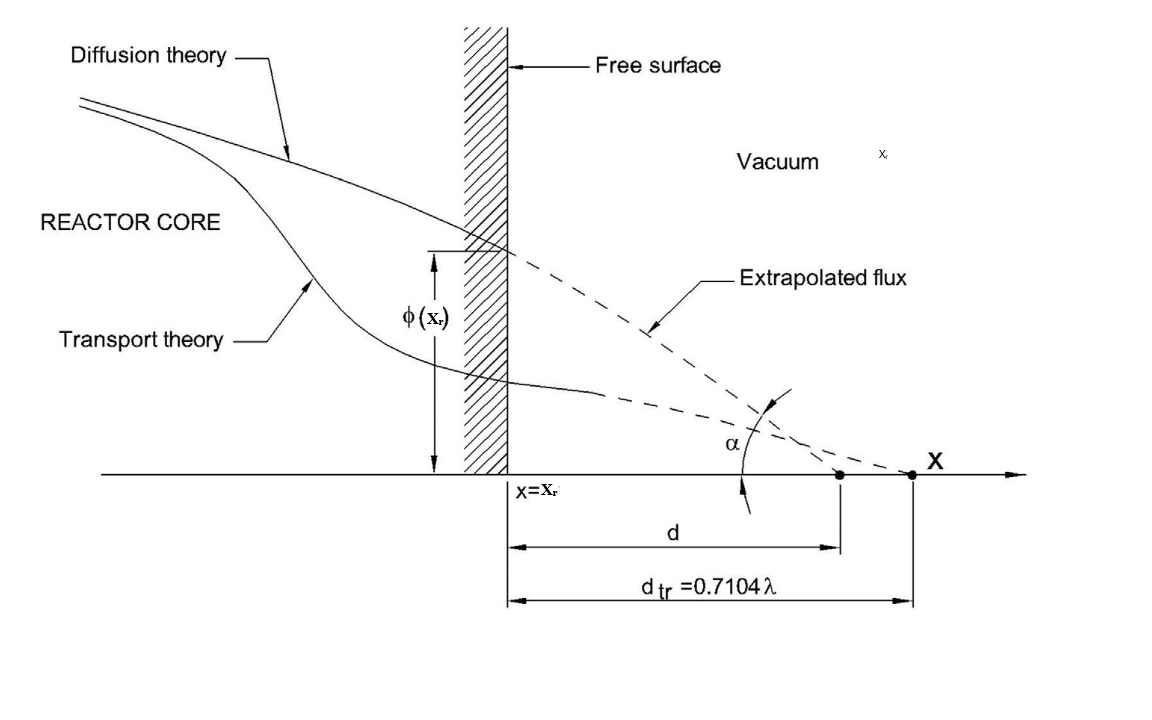
\includegraphics[width=0.75\linewidth]{Kap4/Figures_Kap4/extrapolated_bc_edit.png}
    \caption{Extrapolated boundary conditions. Source: \cite{book_science_direct}}
    \label{fig:extrapolated_bc}
\end{figure}

\section{Non-Leakage Probability}

Finally, to determinate the non-leakage probability lets consider a multiplicative system (\(\nu\Sigma_{f} > 0\)) and a uniform system which means the source \(S'''(r) = S_{0}'''\), \(D(\Vec{r}) = D = cte\) and all cross section are space-independent constants. Additionally, let \(L = \sqrt{D/\Sigma_{a}}\) and \(k_{\infty}\) as in equation (\ref{eq:def_infty_sigmas}). Including all of these in the diffusion equation (\ref{eq:diffusion_equation}) yields:

\begin{flalign}
    && - \nabla^{2} \phi(\Vec{r}) + \frac{1}{L^{2}} \phi(\Vec{r}) = \frac{1}{D}s_{0}''' + \frac{1}{L^{2}}k_{\infty}\phi(\Vec{r}) &&
    \label{eq:std_diffusion}
\end{flalign}

\subsection{Spherical Geometry}

In spherical geometry, the Laplacian \(\nabla^{2}\) is replaced by:

\begin{flalign*}
    && - \frac{1}{r^{2}} \frac{d}{dr}\left( r^{2} \frac{d\phi}{dr} \right) + \frac{1}{L^{2}} (1 - k_{\infty}) \phi = \frac{1}{D} S_{0}''' &&
\end{flalign*}

The solution to this equation is a superposition of the general and particular solutions, \(\phi(r) = \phi_{g}(r) + \phi_{p}(r)\). Assuming a uniform source, we have \(\phi_{p}(r) = \text{const} = \frac{S_{0}'''}{(1 - k_{\infty}) \Sigma_{a}}\) \cite{Lewis_2014}.

For the general solution, consider the case where \(k_{\infty} < 1\). The equation becomes:

\begin{flalign*}
    && \frac{1}{r^{2}} \frac{d}{dr} \left( r^{2} \frac{d\phi_{g}}{dr} \right) - \frac{1}{L^{2}} (1 - k_{\infty}) \phi_{g} = 0 &&
\end{flalign*}

Applying the previously discussed boundary conditions, the solution is:

\begin{flalign*}
    && \phi(r) = \frac{S_{0}'''}{(1 - k_{\infty}) \Sigma_{a}} \left[ 1 - \frac{\Tilde{R} \sinh(\kappa r)}{r \sinh(\kappa \Tilde{R})} \right] &&
\end{flalign*}

where \(\kappa = \frac{1}{L} \sqrt{1 - k_{\infty}}\) and \(\Tilde{R} = R + \frac{2}{3} \lambda\), representing the extrapolated boundary conditions.

Now consider the supercritical case \(k_{\infty} > 1\), where the particular solution is:

\begin{flalign*}
    && \phi_{p} = - \frac{S_{0}'''}{(k_{\infty} - 1)\Sigma_{a}} &&
\end{flalign*}

Solving the general equation and applying the boundary conditions, the solution is:

\begin{flalign*}
    && \phi(r) = \frac{S_{0}'''}{(k_{\infty} - 1)\Sigma_{a}} \left[ \frac{\Tilde{R} \sin(Br)}{r \sin(B \Tilde{R})} - 1 \right] &&
\end{flalign*}

where \(B = \frac{1}{L} \sqrt{k_{\infty} - 1}\).

\subsubsection{Criticality Condition}

In the supercritical solution, consider the limit \(\lim_{B\Tilde{R} \to \pi} \phi_{p} \to \infty\), implying that the sphere becomes critical \cite{Lewis_2014}. The condition for criticality is then:

\[
\frac{1}{L} \sqrt{k_{\infty} - 1} \Tilde{R} = \pi
\]

Solving for \(k_{\infty}\) gives:

\[
k_{\infty} = 1 + \frac{\pi^{2} L^{2}}{\Tilde{R}^{2}}
\]

For a finite reactor, the criticality condition is \(k = P_{NL} k_{\infty} = 1\). Thus, for the critical sphere, the non-leakage probability is:

\begin{flalign}
    && P_{NL} = \frac{1}{1 + \left( \frac{\pi L}{\Tilde{R}} \right)^2} &&
\end{flalign}

Now lets define two new variables. First, the material buckling defined as \(B_{m} = \frac{1}{L}\sqrt{k_{\infty-1}}\) and secondly the geometrical buckling \(B_{g} = \pi/\Tilde{R}\). With this the criticality condition can be expressed as:

\begin{flalign*}
    && B_{m} = B_{g} &&
\end{flalign*}

\subsection{Time-Independent Diffusion Equation}

If we set the source to be zero, then the steady diffusion equation (\ref{eq:diffusion_equation}) becomes:

\begin{flalign}
    && \nabla \cdot D(\Vec{r})\nabla\phi(\Vec{r}) + \nu \Sigma_{f}\phi(\Vec{r}) - \Sigma_{a}\phi(\Vec{r}) = 0 &&
    \label{eq:time_ind_diffusion}
\end{flalign}

In this equation, \(\phi\) tends to zero if the reactor is subcritical. Conversely, if the reactor is in a supercritical state, \(\phi\) tends to infinity. In either case, the kinetic equations (\ref{eq:kinetic_eq_1}) and (\ref{eq:kinetic_eq_2}) are necessary to describe the system's behavior \cite{Lewis_2014}. The challenge is to determine the critical state by varying the reactor's geometry or its material composition \cite{Lewis_2014}. 

To compute this, we apply the following approach: suppose it is possible to adjust the average number of neutrons produced per fission (\(\nu\)) by a factor \(\nu_{0}/\nu\), where \(\nu_{0}\) is the number of neutrons per fission required to bring the reactor to a critical state \cite{Lewis_2014}. Since \(k \sim \nu\), we have \(\nu_{0}/\nu = 1/k\) \cite{Lewis_2014}. Thus, the time-independent diffusion equation (\ref{eq:time_ind_diffusion}) can be rewritten as:

\begin{flalign}
    && \nabla \cdot D(\Vec{r}) \nabla \phi(\Vec{r}) + \frac{1}{k} \nu \Sigma_{f} \phi(\Vec{r}) - \Sigma_{a} \phi(\Vec{r}) = 0 &&
    \label{eq:eigen_diffusion_equation}
\end{flalign}

It is easy to see that if \(\nu_{0} > \nu\), then the reactor is subcritical. On the other hand, if \(\nu_{0} < \nu\), the reactor is supercritical. By incorporating this adjustment into the diffusion equation and solving for \(k\), we transform the problem into finding how far a given configuration (defined by the reactor core's dimensions and cross-sections) is from criticality. 

This can be framed as an eigenvalue problem, where \(k\) is the eigenvalue and \(\phi\) is the eigenfunction. Typically, these problems have an infinite set of solutions. However, by applying the boundary conditions and focusing on physically meaningful solutions, those in which the neutron flux is positive everywhere within the reactor, we narrow the problem to the relevant solution. This solution corresponds to the largest eigenvalue, the corresponding eigenfuntion \(\phi\) is refered as the fundamental mode solution.

\subsubsection{Uniform Reactors}

Now suppose that the reactor is uniform, which implies that \(D\) is constant. Using the same definitions for \(k_{\infty}\) and \(L^{2}\) as in equation (\ref{eq:std_diffusion}), the diffusion equation (\ref{eq:eigen_diffusion_equation}) can be written as:

\begin{flalign*}
    && \nabla^{2}\phi + \frac{k_{\infty}/k - 1}{L^{2}} \phi = 0 &&
\end{flalign*}

Since the term multiplying \(\phi\) is constant, we define \(B^{2} = \frac{k_{\infty}/k - 1}{L^{2}}\). From this equation, it can be shown that the non-leakage probability \(P_{NL}\) is:

\[
P_{NL} = \frac{1}{1 + (LB)^{2}}
\]

Here, \(B\) is referred to as the geometric buckling, or simply the buckling \cite{Lewis_2014}. To determine the buckling, we must solve the following equation, which is the Helmholtz equation:

\begin{flalign}
    && \nabla^{2}\phi + B^{2} \phi = 0 &&
    \label{eq:helmholtz_buckling}
\end{flalign}

The solution must satisfy the condition \(0 < \phi < \infty\) within the reactor, as well as the boundary conditions at the reactor's surfaces \cite{Lewis_2014}.


\subsection{Cylindrical Reactor}

Given a cylindrical reactor with an extrapolated radius \(\Tilde{R} = R + \frac{2}{3} \lambda\) and height \(\Tilde{H} = H + \frac{4}{3} \lambda\), we now examine the buckling. Replacing \(\nabla^2\) in equation (\ref{eq:helmholtz_buckling}) with its form in cylindrical coordinates gives:

\begin{flalign*}
    && \frac{1}{r}\frac{\partial}{\partial r} \left( r\frac{d\phi}{dr} \right) + \frac{\partial^{2}}{\partial z^{2}} \phi + B^{2}\phi = 0 &&
\end{flalign*}

This equation corresponds to a partial differential equation that can be solved by separating variables. Assuming the solution takes the form \(\phi(r, z) = \psi(r) \chi(z)\), substituting and dividing by \(\phi\) yields:

\begin{flalign*}
    && \frac{1}{\psi} \frac{d}{dr} \left( r\frac{d\psi}{dr} \right) + \frac{1}{\chi} \frac{d^{2}\chi}{dz^{2}} + B^{2} = 0 &&
\end{flalign*}

Since \(B^{2}\) is a constant, the first term depends only on \(r\), and the second term depends only on \(z\), meaning each term must equal a constant for the equation to have a solution. Thus, we assume that the total buckling can be written as \(B_{r}^{2} + B_{z}^{2} = B^{2}\). These constants must satisfy the following differential equations:

\begin{flalign*}
    && \frac{d}{dr}\left( r\frac{d\psi}{dr} \right) + B_{r}^{2} \psi = 0 && \\
    && \frac{d^{2}\chi}{dz^{2}} + B_{z}^{2} \chi = 0 &&
\end{flalign*}

Solving these equations gives the expressions \(B_{z} = \pi/\Tilde{H}\) and \(B_{r} = 2.405/\Tilde{R}\). Thus, the total buckling is:

\begin{flalign}
    B^{2} = \left( \frac{2.405}{\Tilde{R}} \right)^{2} + \left( \frac{\pi}{\Tilde{H}} \right)^{2}
    \label{eq:cylindrical_buckling}
\end{flalign}

Although spherical reactors are the most efficient due to their higher non-leakage probability (\(P_{NL}\)), they represent significant technical challenges, such as structural complexity and cooling issues \cite{Notas_sanabricas}. This is why most commercial reactors have cylindrical geometry. 

In the next chapter, we will explore the different fuels used in reactors, examining how they are managed before, during, and after reactor operation.

\chapter{Nuclear fuel cycles}

Now we will examine the life cycle of the materials used as fuel in nuclear reactors. The fuel cycle spans from the mining of the ore to the fabrication of the fuel, its irradiation in the reactor, and the subsequent processing of the spent nuclear fuel \cite{fuel_cycle_book}. The nuclear fuel cycle can vary depending on several factors, such as:

\begin{itemize}
    \item The fissile nuclei being used for energy generation, such as any of the isotopes mentioned in \textbf{Section} \ref{sec:possible_fuels}.
    \item The form in which the fuel is utilized.
    \item The type of reactor in which the fuel is deployed.
\end{itemize}

The nuclear fuel cycle begins with uranium mining and ends with the disposal of nuclear waste \cite{fuel_cycle_book}, although some steps may not apply to every fuel cycle.

\section{Frontend of Fuel Cycle}

The steps involving mining, milling, conversion, enrichment, and fuel fabrication correspond to the ``frontend'' of the nuclear fuel cycle. Uranium-rich minerals are radioactive primarily due to the daughter products derived from radioactive decays of uranium. In 2019, global uranium production was approximately 54,750 tons, with most of the mined uranium being used as fuel for nuclear power plants \cite{fuel_cycle_book}.

Uranium recovery is achieved through extraction from ores, followed by concentration and purification. This process involves both excavation and in-situ leaching (ISL). Typically, open-pit mining is used for deposits near the surface, while underground mining is applied for deeper deposits \cite{fuel_cycle_book}. The mined uranium ore is then processed by grinding, followed by uranium leaching using either alkaline or acidic methods. The milling process yields ``yellowcake'', which contains uranium in the form of \(U_3O_8\), with a uranium content greater than \(80 \, \%\) \cite{fuel_cycle_book}.

Approximately 200 tons of \(U_3O_8\) are required to fuel a 1000 MWe nuclear power reactor for one year. The \(U_3O_8\) produced from the uranium mill is further enriched to increase the \(U^{235}\) content from \(0.72 \, \%\) to between \(3 \, \%\) and \(5 \, \%\), which is required for light water reactors. The enrichment process involves converting uranium into uranium hexafluoride (\(UF_6\)), which is solid at room temperature but sublimates at 56.5°C, allowing it to be used in isotope separation \cite{fuel_cycle_book}.

The primary method used for isotope enrichment today is centrifugation, where thousands of rapidly spinning vertical tubes exploit the small mass difference between the uranium isotopes' hexafluorides, leading to their separation \cite{fuel_cycle_book}.

However the \(UF_6\) is not suitable to be used as fuel in a nuclear reactors, hence needs to be converted to ceramic pellets of \(UO_2\) sintered at temperatures over the \(1400^{\circ}C\). Other pallets composed by a mixed of U, Pu oxide (MOX) are fabricated \cite{fuel_cycle_book}. Currently, conventional UOX fuel have an additive less than \(10 \, \%\) of thorium . This increases the thermal distribution by reducing the need of poison in the reactor \cite{Th_cycle_viability}.

\section{Backend of Fuel Cycle}

The processes that occur after the discharge of irradiated fuel from the reactor, such as the temporary storage of spent fuel, reprocessing, and waste management, are collectively known as the ``backend'' of the nuclear fuel cycle. The energy realised by fission extracted from the fuel is measured as the ``burn up'' \cite{fuel_cycle_book}. The most commonly used metric for fuel burn-up is the amount of fission energy produced per unit mass of fuel. This is expressed as the total energy released, measured in megawatt-days, divided by the initial mass of fuel, including both fissile and fertile materials, and is referred to as \textit{megawatt-days per ton} \((MWd/T)\) \cite{nuclear_reactors_adv}. Since natural uranium contains only \(0.72 \, \%\) of the fissile isotope \(\prescript{235}{}{U}\), the burn-up of fuel based on natural uranium is expected to be below \(0.72 \, atom \, \%\). However, due to the breading of \(\prescript{239}{}{Pu}\) from neutron absorption in \(\prescript{238}{}{U}\), burn-up can achieve values of up to \(1 \, \text{atom} \%\) \((10,000 \, MWd/T)\) \cite{fuel_cycle_book}. In typical pressurized heavy water reactors (PHWRs), the burn-up level is around \(7000 \, MWd/T\). For light water reactors (LWRs) using enriched uranium, burn-up levels can reach \(6–7 \, \text{atom} \, \%\), while in fast reactors, burn-up can exceed \(10 \, \text{atom} \%\), reaching in some cases burn-up as high as \(20 \, \text{atom} \%\) has been achieved \cite{fuel_cycle_book}.

However, fuel burn-up is limited by the accumulation of fission products and actinides, which absorb neutrons and negatively impact neutron economy, leading to a decrease in the reactor's efficiency. This necessitates the removal of the fuel from the reactor. Nevertheless, a typical fuel based on low enrichment uranium (LEU) still contains \(96 \, \%\) of its original uranium content, approximately \(1 \, \%\) of plutonium, and \(3 \, \%\) of fission products and minor actinides \cite{fuel_cycle_book}. Thus, regardless of the type of fuel or reactor, the irradiated fuel remains a valuable source of fissile materials. Even if the uranium is depleted in terms of its fissile content, it can still be used to prepare fuel for a fast reactor by adding plutonium. Therefore, the fuel discharged from a nuclear reactor, although commonly referred to as ``spent fuel'', is not truly ``spent'' as it still contains fissionable materials \cite{fuel_cycle_book}. 

\subsection{Reprocessing}

Reprocessing methods for reprocessing discharged fuel have been developed and used either at the research stage or commercial scale for uranium and thorium based fuels. Some methods are \cite{Th_cycle_viability}:

\begin{itemize}
    \item Pyrometallurgy: This method utilizes heat to initiate the separation of metals from their minerals. 
    \item Electrometallurgy: Also known as pyroprocessing, this technique employs electricity to initiate the separation of metals. However, it is still in the research stage \cite{Th_cycle_viability}.
    \item Hydrometallurgy: This widely used method involves the use of an aqueous solution to dissolve the metal content. In the case of uranium and plutonium extraction, hydrometallurgy utilizes a solution containing \(30\%\) tri-n-butyl phosphate (TBP) in an aliphatic hydrocarbon diluent, such as kerosene or a mixture of normal paraffinic hydrocarbons, to preferentially extract U and Pu. Popularly known as PUREX by the acronym: Plutonium Uranium Redox EXtraction \cite{fuel_cycle_book}.
\end{itemize}

\subsection{Waste Management}

Radioactive waste management is a crucial aspect of the nuclear energy program. The common strategy for managing radioactive waste involves vitrification, where solid waste oxides are encapsulated in borosilicate glass blocks. These glass blocks are then buried in deep geological repositories (DGRs). However, this disposal method requires long-term surveillance due to the very long half-lives of minor actinides (such as neptunium, americium, and curium) and some fission products, making the waste management program highly expensive \cite{fuel_cycle_book}.

The decay of buried radionuclides takes millions of years, and it takes a significant amount of time for the radiotoxicity of long-lived radionuclides present in the waste blocks to reduce to a level comparable to that of natural uranium from natural sources\cite{fuel_cycle_book}. To address these challenges, processes for partitioning of minor actinides such as Np, Am, and Cm, as well as fission products have been developed. These processes aim to reduce the average exposure to operating personnel and can be followed by the transmutation of long-lived radionuclides in fast reactors or accelerator-driven sub-critical systems (ADS) \cite{fuel_cycle_book}.

The strategy of ``Actinide Partitioning'' combined with other emerging strategies such as ``lanthanide-actinide separation'' and ``Am-Cm separation'' offers additional benefits, including the recovery of valuable materials like Am and Cm \cite{fuel_cycle_book}. In the long term, the ``Partitioning \& Transmutation'' (\(P\&T\)) strategy effectively addresses concerns about radioactive waste management and provides a potential solution for reducing the radiotoxicity of long-lived radionuclides \cite{fuel_cycle_book}.

\section{Fuel Cycles}

The nuclear fuel cycle can be classified into two main categories: open and closed fuel cycles. The open fuel cycle is characterized by the use of nuclear fuel without reprocessing, while the closed fuel cycle involves reprocessing the spent fuel to recover fissile materials for reuse in the reactor. The open fuel cycle is also known as the ``once-through'' fuel cycle, as the fuel is reprocessed and reused in the reactor until it is no longer economically viable \cite{fuel_cycle_book}.

\subsection{Open Fuel Cycle}

The open fuel cycle is the simplest and most common fuel cycle used in commercial nuclear power plants. In this cycle, the fuel is used in the reactor only once, then discharged and stored in interim storage facility where it is kept until most of the short-lived material has decayed. The spent fuel is stored in a DGR for long-term disposal. The open fuel cycle is used in the USA, UK and South Africa \cite{fuel_cycle_book}.

\subsubsection{Twice-Through Fuel Cycle}

This cycle reprocess the spent fuel to recover uranium and plutonium for reuse in the reactor. MOX is fabricated from the reprocessed fuel and then used in the reactor for a second time before being disposed of in a DGR similar to the ``once-through'' cycle \cite{fuel_cycle_book}. The major reason for recycling of the “spent nuclear fuel” (SNF) in the case of the “twice-through” NFC is due to the fact that the SNF still contains approximately \(96\%\) of the reusable material (U and Pu) and, hence, is still considered as an energy source due to its appreciable fissile material content. Additional cycles in a thermal reactor are not practical due to degradation of the isotopic composition of Pu \cite{fuel_cycle_book}.

As compared to the “once-through” NFC, in which the SNF is stored after use and buried in DGRs after vitrification, the “twice-through” NFC can utilize \(17 \, \%\) more natural uranium by the MOX fuel option, which can largely discount the heavy enrichment costs \cite{fuel_cycle_book}. 

\subsection{Closed Fuel Cycle}

The objective of the closed fuel cycle is effective utilization of fissile materials and the reduction of long-lived radioactive waste. The closed fuel cycle requires the development of advance technologies for reprocessing to achieve a sustainable NFC \cite{fuel_cycle_book}. 

\subsubsection{Closed Fuel Cycle without MA Recovery}

In a closed fuel cycle with minor actinide and fission product recovery, uranium and plutonium are extracted from the irradiated fuel. The separated plutonium can be reused in thermal or fast reactors, while the depleted uranium can be utilized in MOX fuels for both types of reactors. This approach was initially implemented by countries with limited uranium reserves, aiming to recover and utilize the depleted uranium and plutonium from the discharge fuel \cite{fuel_cycle_book}.


\subsubsection{Closed Fuel Cycle with MA Recovery}

The recovery of minor actinides often involves the simultaneous recovery of lanthanides due to the similar chemical properties. These recovered minor actinides can then be burned in ADSs or fast reactors. In this context, the separation of lanthanides from actinides, followed by the separation of americium from curium, has become an important step for the effective transmutation of long-lived actinides. It is essential, however, that the recovery of radiotoxic minor actinides be nearly \(100 \, \%\) effective in order to simplify waste immobilization and ensure the remnant waste qualifies as "non-alpha" waste for disposal in DGRs \cite{fuel_cycle_book}.

\subsubsection{Closed Fuel Cycle with MA and Fission Product Recovery}

Fission products constitute about \(0.6 \, \%\) of the irradiated fuel, with long-lived fission products making up only around \(0.04 \, \%\). Although they are present in small quantities, the main source of radioactivity in HLLW comes from highly radioactive fission nuclides like \(\prescript{137}{}{Cs}\) and \(\prescript{90}{}{Sr}\), which are responsible for the majority of the radiation dose. 

Other radionuclides, such as \(\prescript{106}{}{Ru}\) with moderate activity, and long-lived fission products like \(\prescript{99}{}{Tc}\), \(\prescript{93}{}{Zr}\), \(\prescript{135}{}{Cs}\), \(\prescript{129}{}{I}\), and \(\prescript{107}{}{Pd}\), also contribute to the overall radioactivity \cite{fuel_cycle_book}.

Some of these fission products, such as \(\prescript{90}{}{Y}\) are useful in nuclear medicine. This has led to efforts to separate these radionuclides from HLLW before vitrification. In addition, long-lived fission products can be transmuted into shorter-lived ones to reduce the time required for monitoring vitrified waste. In India, the current strategy involves separating fission products prior to the actinide partitioning step \cite{fuel_cycle_book}.


\chapter{Thorium Fuel Cycle}

Thorium based nuclear fuel have been of interest from 1950 to 1970 \cite{Th_cycle_viability}. This led to the development of multiple experimental reactors that could operate with thorium based fuel \cite{TMSR_book}. In the 1950, thorium was of special interest due to its higher abundance compared to uranium, being three times more abounded than uranium \cite{Th_cycle_viability,TMSR_book}.

The thorium fuel cycle is based on the use of \(\prescript{232}{}{Th}\) as fertile material, which is converted into fissile \(\prescript{233}{}{U}\) by neutron capture and beta decay. This implies that an additional step of converting the fertile isotope into the fissile material is required. The subsequent use of \(\prescript{233}{}{U}\) as fuel is possible in two ways. The first option is an open fuel cycle, based of the breading of \(\prescript{233}{}{U}\) and in situ fission of this isotope, this would not involve chemical separation of \(\prescript{233}{}{U}\) from the irradiated fuel \cite{IAEA_Th_Potential}. The second option is a closed fuel cycle, where the irradiated fuel is reprocessed to separate the fissile material from the rest of the irradiated fuel, this fissile material is then used to fabricate new fuel elements \cite{IAEA_Th_Potential}. 

\section{Considerations for the Thorium Fuel Cycle}

The chemical properties of thorium make thorium dioxide more stable and has higher radiation resistance than uranium dioxide \cite{IAEA_Th_Potential}. \(ThO_2\) has higher thermal conductivity and lower coefficient of thermal expansion compared to \(UO_2\), this might make \(ThO_2\) based fuels to have a better in-pile perform \cite{IAEA_Th_Potential}. Furthermore, \(ThO_2\) is considered inert and does not oxidize unlike \(UO_2\), making long term storage of irradiated fuel easier \cite{IAEA_Th_Potential}.

The thorium fuel cycle has a higher conversion ratio in thermal reactors compared to the uranium fuel cycle, this is due to the fact that \(\prescript{232}{}{Th}\) has a higher neutron capture cross section compared to \(\prescript{238}{}{U}\) with thermal neutrons \cite{IAEA_Th_Potential}. Additionally, the fraction of neutrons liberated per neutron absorbed (\(\eta\)) is greater than \(2.0\) over a wide range of thermal neutron, unlike \(\prescript{235}{}{U}\) and \(\prescript{239}{}{Pu}\). Making \(\prescript{232}{}{Th} - \prescript{233}{}{U}\) operational with fast or thermal spectra. Unlike \(\prescript{238}{}{U} - \prescript{239}{}{Pu}\) which a breading chain reaction can only be obtained with fast neutrons \cite{IAEA_Th_Potential}.

Finally, the thorium fuel cycle has ``intrinsic proliferation resistance'' \cite{IAEA_Th_Potential}. This is because of the formation of \(\prescript{232}{}{U}\) via neutron multiplication reactions (\(n,2n\)) with \(\prescript{232}{}{Th}, \prescript{233}{}{Pa}\) and \(\prescript{233}{}{U}\). \(\prescript{232}{}{U}\) has physical properties, such as a very short half-life (\(t_{1/2} = 68.90 \, \text{years} \)) and the emission of strong gamma radiation by its decay products \cite{IAEA_Th_Potential,NNDC}. This makes the thorium fuel cycle less attractive for the production of nuclear weapons \cite{IAEA_Th_Potential}.

\section{Thorium Front End}

All thorium isotopes have short half-lives, except \(\prescript{232}{}{Th}\) which has a half-life of \(t_{1/2} = 1.405 \times 10^{10} \, \text{years}\) \cite{NNDC}, making all the natural thorium available on earth constituted by \(\prescript{232}{}{Th}\). Generally, Natural thorium is presented in association with other elements, such as rare earths elements and uranium in diverse rocks types such as veins of thorite, thorianite, uranothorite and  monazite in granites and other acidic intrusions \cite{IAEA_Th_Potential}. 

The global thorium reserves to \(2013\) are estimated to be around \(6.24 \, \text{million tons}\). India has the largest thorium reserves, with approximately \(846,000 \, \text{tons}\), followed by Brazil with \(632,000 \, \text{tons}\) and the United States with \(595,000 \, \text{tons}\) \cite{Th_cycle_viability}.

Thorium reserves in Colombia are associated mainly with igneous rocks, such as granites and pegmatites, and can also be found in placers, especially in alluvial deposits \cite{Th_Colombia}. The concentration of thorium in the country varies significantly depending on the geological formation, with values ranging between \(0.1\) and \(585 \, \text{mg}/\text{kg}\) in sediments. The highest concentrations are observed in areas with granitic formations, such as the Sierra Nevada de Santa Marta and parts of the Andean region, which are known for their igneous and metamorphic rocks \cite{Th_Colombia}. 

The mining and extraction of thorium from monazite is relatively straightforward and differs significantly from the extraction of uranium from its ores. Most commercially exploited monazite comes from beach or river sands, often alongside other heavy minerals. Compared to uranium mining, thorium extraction involves much less overburden, and the radioactive waste produced is approximately two orders of magnitude lower. The so-called radon impact is also considerably smaller for thorium mining, due to the shorter half-life of thoron (\(\prescript{220}{}{Rn}\)) compared to radon (\(\prescript{222}{}{Rn}\)), leading to simpler tailings management \cite{IAEA_Th_Potential,Thoron}.

The monazite is finely ground and dissolved in concentrated sodium hydroxide at around \(140^{\circ}C\), followed by a series of chemical processes, including solvent extraction and ion exchange, to yield pure thorium nitrate. This is then precipitated as thorium oxalate and calcined to obtain \(ThO_2\) powder. Thorium recovery projects typically separate thorium in pure oxalate form, which is easier to handle and store for future applications, such as preparing mantle-grade thorium nitrate or nuclear-grade thorium oxide. Uranium present in monazite is also separated in the form of crude uranium concentrate during the process \cite{IAEA_Th_Potential}.

\section{Thorium Open Fuel Cycle}

An open fuel cycle avoids the complex engineering requirements associated with reprocessing irradiated fuel and fabricating highly radiotoxic \(\prescript{233}{}{U}\)-based fuels. The core layout is designed such that each fuel assembly comprises a ``seed'' material, typically medium-enriched uranium or plutonium, and ``blanket'' material of thorium \cite{IAEA_Th_Potential}. Separation of seed and blanket, optimization moderator to fuel ratio and long periods of fuel usage offer the possibility that around \(40 \, \%\) of the power generated by fission comes from \(\prescript{233}{}{U}\) \cite{IAEA_Th_Potential}.

This scheme is very attractive for an introduction if thorium in nuclear power reactors because of the direct utilization of \(\prescript{233}{}{U}\), avoiding the need of reprocessing and fabrication of new fuel elements with \(\prescript{233}{}{U}\) \cite{IAEA_Th_Potential}. Furthermore, the once-through thorium fuel cycle opens the possibility of incineration if weapons-grade plutonium in light water reactors \cite{IAEA_Th_Potential}. To achieve this, thorium oxide containing \(5 \, \%\) of \(PuO_2\), could be used as driver fuel. The exclusion of uranium from the fuel composition results in an increase in the rate of plutonium incineration compared to standard MOX fuel \cite{IAEA_Th_Potential}.

Similarly, civil plutonium could be burned in a thorium fuel cycle by using the same combination of thorium oxide and plutonium oxide \cite{IAEA_Th_Potential}. Since, \(\prescript{240}{}{Pu}\) is present is significant quantities in civil grade plutonium, and it is a good burnable absorbed, then there is no need for use burnable absorber in the form of gadolinium, integrated into the fuel \cite{IAEA_Th_Potential}. Plutonium oxide fuel without major modification in the reactor core could be a direct replacement for LEU oxide fuel \cite{IAEA_Th_Potential}.

\section{Thorium Closed Fuel Cycle}

The closed fuel cycle for thorium-based fuels includes essential steps such as reprocessing irradiated fuel and separating converted \(\prescript{233}{}{U}\). In some reactor designs, like LWRs, mixed thorium-plutonium oxide fuel is used to facilitate the conversion of \(\prescript{232}{}{Th}\) to \(\prescript{233}{}{U}\). However, an important consideration in recycling \(\prescript{233}{}{U}\) is the presence of \(\prescript{232}{}{U}\), which introduces radiological challenges due to its strong gamma emissions \cite{IAEA_Th_Potential}.

Various countries have implemented closed thorium fuel cycles. In Russia, fast breeder reactors like the BN-800 have been studied for their capability to achieve self-sufficiency in the \(\prescript{232}{}{Th}-\prescript{233}{}{U}\) cycle with a breeding ratio close to or exceeding 1.0. France has also explored similar concepts in reactor types such as high-temperature gas-cooled reactors (HTGRs) and HWRs, finding that these reactors can approach a breeding ratio of 1.0, though not exceed it \cite{IAEA_Th_Potential}.

India has adopted a strategic three-stage nuclear program to maximize its vast thorium reserves. The first stage, utilizing PHWRs, employs \(\text{ThO}_2\) assemblies to flatten neutron flux. The second stage, using liquid metal-cooled fast breeder reactors (LMFBRs), incorporates \(\text{ThO}_2\) blankets to produce \(\prescript{233}{}{U}\). Finally, the third stage involves advanced thermal reactors that are self-sustaining in \(\prescript{232}{}{Th}-\prescript{233}{}{U}\) fuels, like the Advanced Heavy Water Reactor (AHWR) designed by Bhabha Atomic Research Center (BARC). This multistage program enables India to establish a sustainable thorium cycle by gradually transitioning to a thorium-based closed fuel cycle \cite{IAEA_Th_Potential}.

\subsection{Reprocessing}

The THOREX (Thorium-uranium EXtraction) process is the primary method proposed for reprocessing thorium-based fuels. Developed at Oak Ridge National Laboratory in the 1950s, THOREX uses solvent extraction with tributyl phosphate (TBP) to separate uranium and thorium from fission products. This process builds on the success of TBP in the PUREX process, making it a natural choice for thorium fuel reprocessing. The THOREX process has mainly been implemented at laboratory or pilot scales in a few countries. For example, India established a facility at BARC in 1970 to reprocess thorium irradiated in the CIRUS reactor (Canada India Reactor Utility Services), successfully achieving high-purity \(\prescript{233}{}{U}\) with minimal \(\prescript{232}{}{U}\) contamination \cite{IAEA_Th_Potential,fuel_cycle_book}.

The objective of the THOREX process is to separate and purify \(\prescript{232}{}{Th}\), \(\prescript{233}{}{U}\), and \(\prescript{233}{}{Pa}\) from irradiated thorium fuel, effectively minimizing impurities and contaminants. Despite its technical feasibility, the process has yet to reach the commercial maturity of PUREX, primarily due to engineering challenges such as solvent handling and multiple purification stages. Current research has led to the development of three primary THOREX flowsheets: Interim 23, THOREX-1, and THOREX-2, each offering distinct methods for optimizing separation and improving the efficiency of thorium fuel reprocessing \cite{fuel_cycle_book}.

\subsubsection{Interim 23}

Developed to recover \(\prescript{233}{}{U}\) from irradiated thorium fuel, the Interim 23 process uses \(1.5 \, \%\) TBP in solutions of irradiated thoria (\(ThO_2\)). In this process, silica gel is applied to remove protactinium (\(Pa\)), while Dowex 50 exchange resin is used to concentrate the final product. The process achieves a thorium separation factor of over \(10^5\) with an overall loss of approximately \(0.5\%\). Additionally, solvent extraction provides a fission product separation factor of greater than \(10^5\), which improves to \(10^7\) after the silica gel and concentration steps \cite{fuel_cycle_book}.


\subsubsection{THOREX-1}

The THOREX-1 process was developed with the aim of separating \(\prescript{233}{}{Pa}\), \(\prescript{233}{}{U}\), and \(\prescript{232}{}{Th}\) from irradiated thorium fuel. The process involved multiple stages: diisobutyl carbitol was used specifically for the separation of \(\prescript{233}{}{Pa}\), \(\prescript{233}{}{U}\) extraction was performed with \(5 \, \%\) TBP, and \(\prescript{232}{}{Th}\) extraction required a higher concentration of \(45 \, \%\) TBP. Although the THOREX-1 process achieved adequate decontamination of the products, it encountered significant engineering challenges. These included the complexity of handling different solvents, separate chemical treatments for solvent purification, and managing hot solutions across various processing stages \cite{fuel_cycle_book}.


\subsubsection{THOREX-2}

An alternative TBP-based process for separating \(\prescript{233}{}{U}\) and thorium from irradiated thorium fuel has been developed. This method uses a single TBP solvent system with concentrations between \(41 \, \%\) and \(55 \, \%\) for the initial separation of thorium and uranium. The process begins under slightly acidic conditions, intentionally kept low to minimize the extraction of protactinium and fission products while avoiding thorium precipitation. To ensure Pa remains in the high-active waste stream, an aluminum nitrate scrub solution is added, maintaining a mildly acidic environment. Separation of thorium from uranium is achieved through selective stripping with dilute nitric acid, and \(\prescript{233}{}{U}\) is removed using a very low-concentration nitric acid solution \cite{fuel_cycle_book}. 

Careful regulation of flow rates is necessary to prevent third-phase formation, which can complicate thorium separation. This approach avoids the need for benzene as a solvent. Following this, Pa is recovered by adsorption onto a silica gel column, eliminating the need for further adjustments to the feed solution. By adjusting acidity levels and controlling flow rates at each stage, the process maintains effective separation of \(\prescript{233}{}{U}\) and thorium with minimal loss \cite{fuel_cycle_book}.

\subsection{Backend Issues}

The backend of the thorium fuel cycle presents unique challenges that must be addressed before thorium can be widely adopted in commercial reactors. Key issues include the management of radionuclide inventories in spent thorium-based fuels, which may contain various fertile/fissile combinations, such as \(\prescript{232}{}{Th}-\prescript{235}{}{U}-\prescript{238}{}{U}\), \(\prescript{232}{}{Th}-\prescript{239}{}{Pu}\), and \(\prescript{232}{}{Th}-\prescript{233}{}{U}\). An understanding of the residual heat, radiological impact, and quantities of actinides and long-lived fission products in these spent fuels is essential \cite{IAEA_Th_Potential}.

Several additional challenges complicate the reprocessing of thorium-based fuels. Protactinium (\(\prescript{233}{}{Pa}\)), formed as an intermediate in the conversion of \(\prescript{232}{}{Th}\) to \(\prescript{233}{}{U}\), has a relatively long half-life (27 days) compared to \(\prescript{239}{}{Np}\) in the uranium cycle. This requires a cooling period of around 12 months to allow \(\prescript{233}{}{Pa}\) to decay to \(\prescript{233}{}{U}\), avoiding loss of fissile material. Protactinium, often relegated to the waste stream, also introduces radiological concerns due to \(\prescript{231}{}{Pa}\), a long-lived alpha emitter in the thorium chain. Attempts to co-extract Pa with U and Th in the \(HNO_3–TBP/\text{kerosene}\) process have been unsuccessful, though a selective adsorption technique using Vycor glass has shown promise, achieving approximately \(98 \, \%\) separation of protactinium \cite{IAEA_Th_Potential}.

The presence of \(\prescript{232}{}{U}\) in spent thorium fuel is another concern. \(\prescript{232}{}{U}\), formed through neutron interactions with \(\prescript{232}{}{Th}\) and its products, decays into gamma-emitting daughters like \(\prescript{208}{}{Tl}\), complicating handling and storage due to the high radiation levels. The \(\prescript{232}{}{U}\) content is influenced by the neutron spectrum and irradiation duration, with fast reactors yielding higher \(\prescript{232}{}{U}\) levels than thermal reactors. Strategies such as positioning thorium blankets away from the core in reactors like the BN-350 have successfully minimized \(\prescript{232}{}{U}\) concentrations in the produced \(\prescript{233}{}{U}\).

Lastly, dissolving thorium dioxide in nitric acid presents challenges, as \(ThO_2\) is highly stable compared to uranium and plutonium oxides. Dissolution generally requires the addition of hydrofluoric acid (HF) to nitric acid, though this accelerates corrosion of processing equipment. The THOREX reagent is the most effective solution developed to date for dissolving Th-based fuels. Higher temperatures and pressures during dissolution also improve the process, addressing this unique aspect of thorium reprocessing \cite{IAEA_Th_Potential}.

\section{Molten Salt Reactors (MSR)}

Currently, most nuclear power plants operate with LWRs, which present several disadvantages. One key issue is the proliferation risk due to the production of \(\prescript{239}{}{Pu}\) in used fuel, which remains a concern whether the fuel is reprocessed or disposed of as waste. Additionally, LWRs have limited thermal efficiency, typically capped at around \(35\,\%\), due to temperature constraints. There is also the risk of steam explosions in these reactors, as well as high core afterheat during accidents, which raises the danger of fuel melting, as observed in incidents like Three Mile Island and Fukushima \cite{TMSR_book}.

MSRs offer promising solutions to many of these challenges. Unlike LWRs, MSRs can operate at low pressures, reducing the risks associated with high-pressure containment and the need for robust, large containment domes. Moreover, MSRs eliminate the need for cladding, which reduces the risk of cladding failure and hydrogen production, a key contributor to explosions in accidents involving high-temperature interactions between zirconium cladding and water. Since the fuel in an MSR is already molten, there is no risk of solid fuel melting during accidents \cite{TMSR_book}.

In addition, MSRs provide advantages such as continuous online refueling and reactivity adjustments, which allow for smoother operation and safer control. They can also maintain lower core excess reactivity, simplifying reactor control. Continuous removal of fission products, such as \(\prescript{137}{}{Cs}\), reduces core radioactivity and mitigates the release of contaminants in severe accidents. Noble gases like xenon and krypton, which cause xenon poisoning in reactors, can be easily removed, avoiding common control issues seen in LWRs \cite{TMSR_book}.

\subsection{Challenges for the Implementation of Molten Salt Reactors}



\chapter{Simulation}
In this project it was simulated a Pressurized Water Reactor (PWR) with different Thorium fuel cycles. The simulation aims to understand the behavior of thorium based nuclear fuels in a PWR. 

\section{Methodology}
The simulation was done using openMC, which is a library for Monte Carlo simulations of neutron transport. The code was developed by the Computational Reactor Physics Group (CRPG) at the Massachusetts Institute of Technology (MIT). 

\subsection{Monte Carlo Method}
The Monte Carlo method is a statistical technique used to solve mathematical problems by generating random samples to obtain numerical results. This method simulates a large number of individual particles and their interactions with materials, then estimates the desired quantities by averaging the results of all particles \cite{TMSR_book}.

The simulation code is written in Fortran 2008 and uses the FoX XML library to process input files in XML format \cite{OpenMC}. XML is used for all inputs because it allows developers to easily modify options, and the FoX library efficiently handles these changes as long as the file structure is well-defined and consistent with the specification files \cite{OpenMC}.

\subsection{OpenMC}
The input files are divided into three mandatory categories for every simulation: settings, materials, and geometry. The settings file contains all simulation parameters, including the number of particles to run. The materials file describes the composition of the materials by densities and elements or nuclei. The geometry file defines the model's geometry \cite{OpenMC}.

However, it is needed to set an additional environment variable to run the code. The environment variable is called ``\texttt{OPENMC\_CROSS\_SECTIONS}'' and it is used to specify the path to the cross-section data. The cross-section data is a library that contains the cross-sections for all isotopes used in the simulation. The library is generated using the ``NJOY'' nuclear data processing code. However, it is also possible to use the cross-section data from the official data libraries like ENDF/B-VII.1 \cite{OpenMC}.

The implemented code uses depletion calculations to simulate the evolution of the fuel composition over time. The depletion calculations are done using the OpenMC depletion capability. The library uses numerical integration to solve the coupled concentration equation known as bateman equations \cite{OpenMC}. Bateman equations are a series of differential equations that describe the time evolution of the concentration of isotopes in a nuclear reactor. The equations are given by:

\begin{flalign}
    && \frac{dN_i(t)}{dt} = \sum_{j} \left[ \int_{0}^{\infty} \sigma_{j \to i}(E,t)\phi(E, t)dE + \lambda_{j \to i} \right] N_{j}(t) && \nonumber \\
    && - \sum_{j} \left[ \int_{0}^{\infty} \sigma_{i \to j}(E,t)\phi(E, t)dE + \lambda_{i \to j} \right] N_{i}(t) &&
\end{flalign}

\vspace{0.5cm}

Where \(N_{i}(t)\) is the number of nuclei of isotope \(i\) at time \(t\), \(\sigma_{j \to i}(E,t)\) is the microscopic cross-section for the reaction where a nucleus of the kind \(j\) generates an isotope of the kind \(i\) \cite{Bateman_equation}. For the depletion calculations, it is necessary to give an additional input file that contains the transmutation reactions and the decay constants for the isotopes. The depletion file is also in XML format \cite{OpenMCweb}.

The results from the depletion calculations are stored in an output file in HDF5 format. The HDF5 format allows parallel writing of the data, make it possible multi threading execution, and is a widely used format for storing large amounts of data. The output file contains the number of nuclei of each isotope at each time step, the k-effective, and the neutron flux \cite{OpenMCweb,HDFGroupDoc}. Additional, information about the output file can be found in the OpenMC documentation \textbf{Ref.}\cite{OpenMCweb}.

\section{Model}
The model used in the simulation is a PWR. It was use the model from the OpenMC example files. The model is a \(17\times17\) fuel assembly from the ``BEAVRS'' benchmark. The model is a 3D model with 3 regions: fuel, water, and cladding. The fuel is a \(UO_2\) fuel with \(3.1 \, \%\) enrichment. The cladding is made of Zircaloy-4 and the water is light water (\(H_2O\)). 

The code is made of two main parts. The first part implements the assembly and defines the nuclear model. In this script settings like the number of particles, the number of batches, and the number of generations are defined. The second part is the depletion script. This script defines the depletion calculations and the output file.

Multiple file for plotting the results are also implemented. The files are written in Python and use the libraries ``numpy'', ``matplotlib'', and ``h5py''. The files read the output file from the depletion calculations and plot the results. The plots show the percentage change in each step of simulation of each isotope. Finally, the plots are saved in a directory called ``plots''. 

\subsection{Project Structure}

The project is organized into several directories and files, each serving a specific purpose:

\begin{tcolorbox}
    Root/: Project root directory.
    \begin{itemize}[itemsep=0pt, parsep=0pt]
        \item Data/: Data files for the simulation.
        \begin{itemize}[itemsep=0pt, parsep=0pt]
            \item \texttt{chain\_endfb80\_pwr.xml}
            \item ...
        \end{itemize}
        \item Plots/: Plot images from simulation results.
        \begin{itemize}[itemsep=0pt, parsep=0pt]
            \item \texttt{percentual\_change\_th232\_con\_10.pdf}
            \item ...
        \end{itemize}
        \item Results/: Simulation results.
        \begin{itemize}[itemsep=0pt, parsep=0pt]
            \item \texttt{Th232/}
            \item ...
        \end{itemize}
        \item Simulation/: Simulation scripts and files.
        \begin{itemize}[itemsep=0pt, parsep=0pt]
            \item \texttt{plotter\_3.py}
            \item \texttt{pwr\_model\_source.py}
            \item \texttt{run\_reactor.py}
            \item ...
        \end{itemize}
        \item \texttt{README.md}: Project documentation.
        \item \texttt{dockerfile}: Docker configuration.
    \end{itemize}
\end{tcolorbox}

The simulation directory contains the core Python scripts essential for the simulation process. The ``\texttt{pwr\_model\_source.py}'' script implements the detailed fuel assembly. The ``\texttt{run\_reactor.py}'' script manages the simulation execution. The ``\texttt{plotter\_3.py}'' script processes the simulation data, generating visual representations of the results. The data directory includes critical files such as depletion chain file. The results directory stores the output files from the simulations, sorting the generated data. 

\section{Results}
Multiple simulations were conducted to evaluate the behavior of the fuel during the operation of the PWR over a period of 6 months. Simulations were performed with various thorium concentrations in uranium oxide fuel, specifically \(10 \, \%\) and \(50 \, \%\). Figures \textbf{Fig.}\ref{fig:th10} and \textbf{Fig.}\ref{fig:th50} illustrate the results of these simulations, showing the percentage change of isotopes in the fuel assembly over the simulation period. The plots indicate the achievement of breeding in the fuel assembly for \(\prescript{233}{}{U}\). However, it is noticeable that the stability of breeding is achieved much later compared to \(\prescript{239}{}{Pu}\). This is expected since the breeding of \(\prescript{233}{}{U}\) follows the chain reaction of \(\prescript{232}{}{Th} \xrightarrow{\substack{\text{neutron} \\ \text{absorption}}} \prescript{233}{}{Th} \xrightarrow{22 \, \text{minutes}} \prescript{233}{}{Pa} \xrightarrow{27 \, \text{days}} \prescript{233}{}{U}\), which is a much slower breading process than the chain reaction of \(\prescript{238}{}{U} \xrightarrow{\substack{\text{neutron} \\ \text{absorption}}} \prescript{239}{}{U} \xrightarrow{23.5 \, \text{minutes}} \prescript{239}{}{Np} \xrightarrow{2.4 \, \text{days}} \prescript{239}{}{Pu}\) for plutonium breading.

\begin{figure}[h]
    \centering
    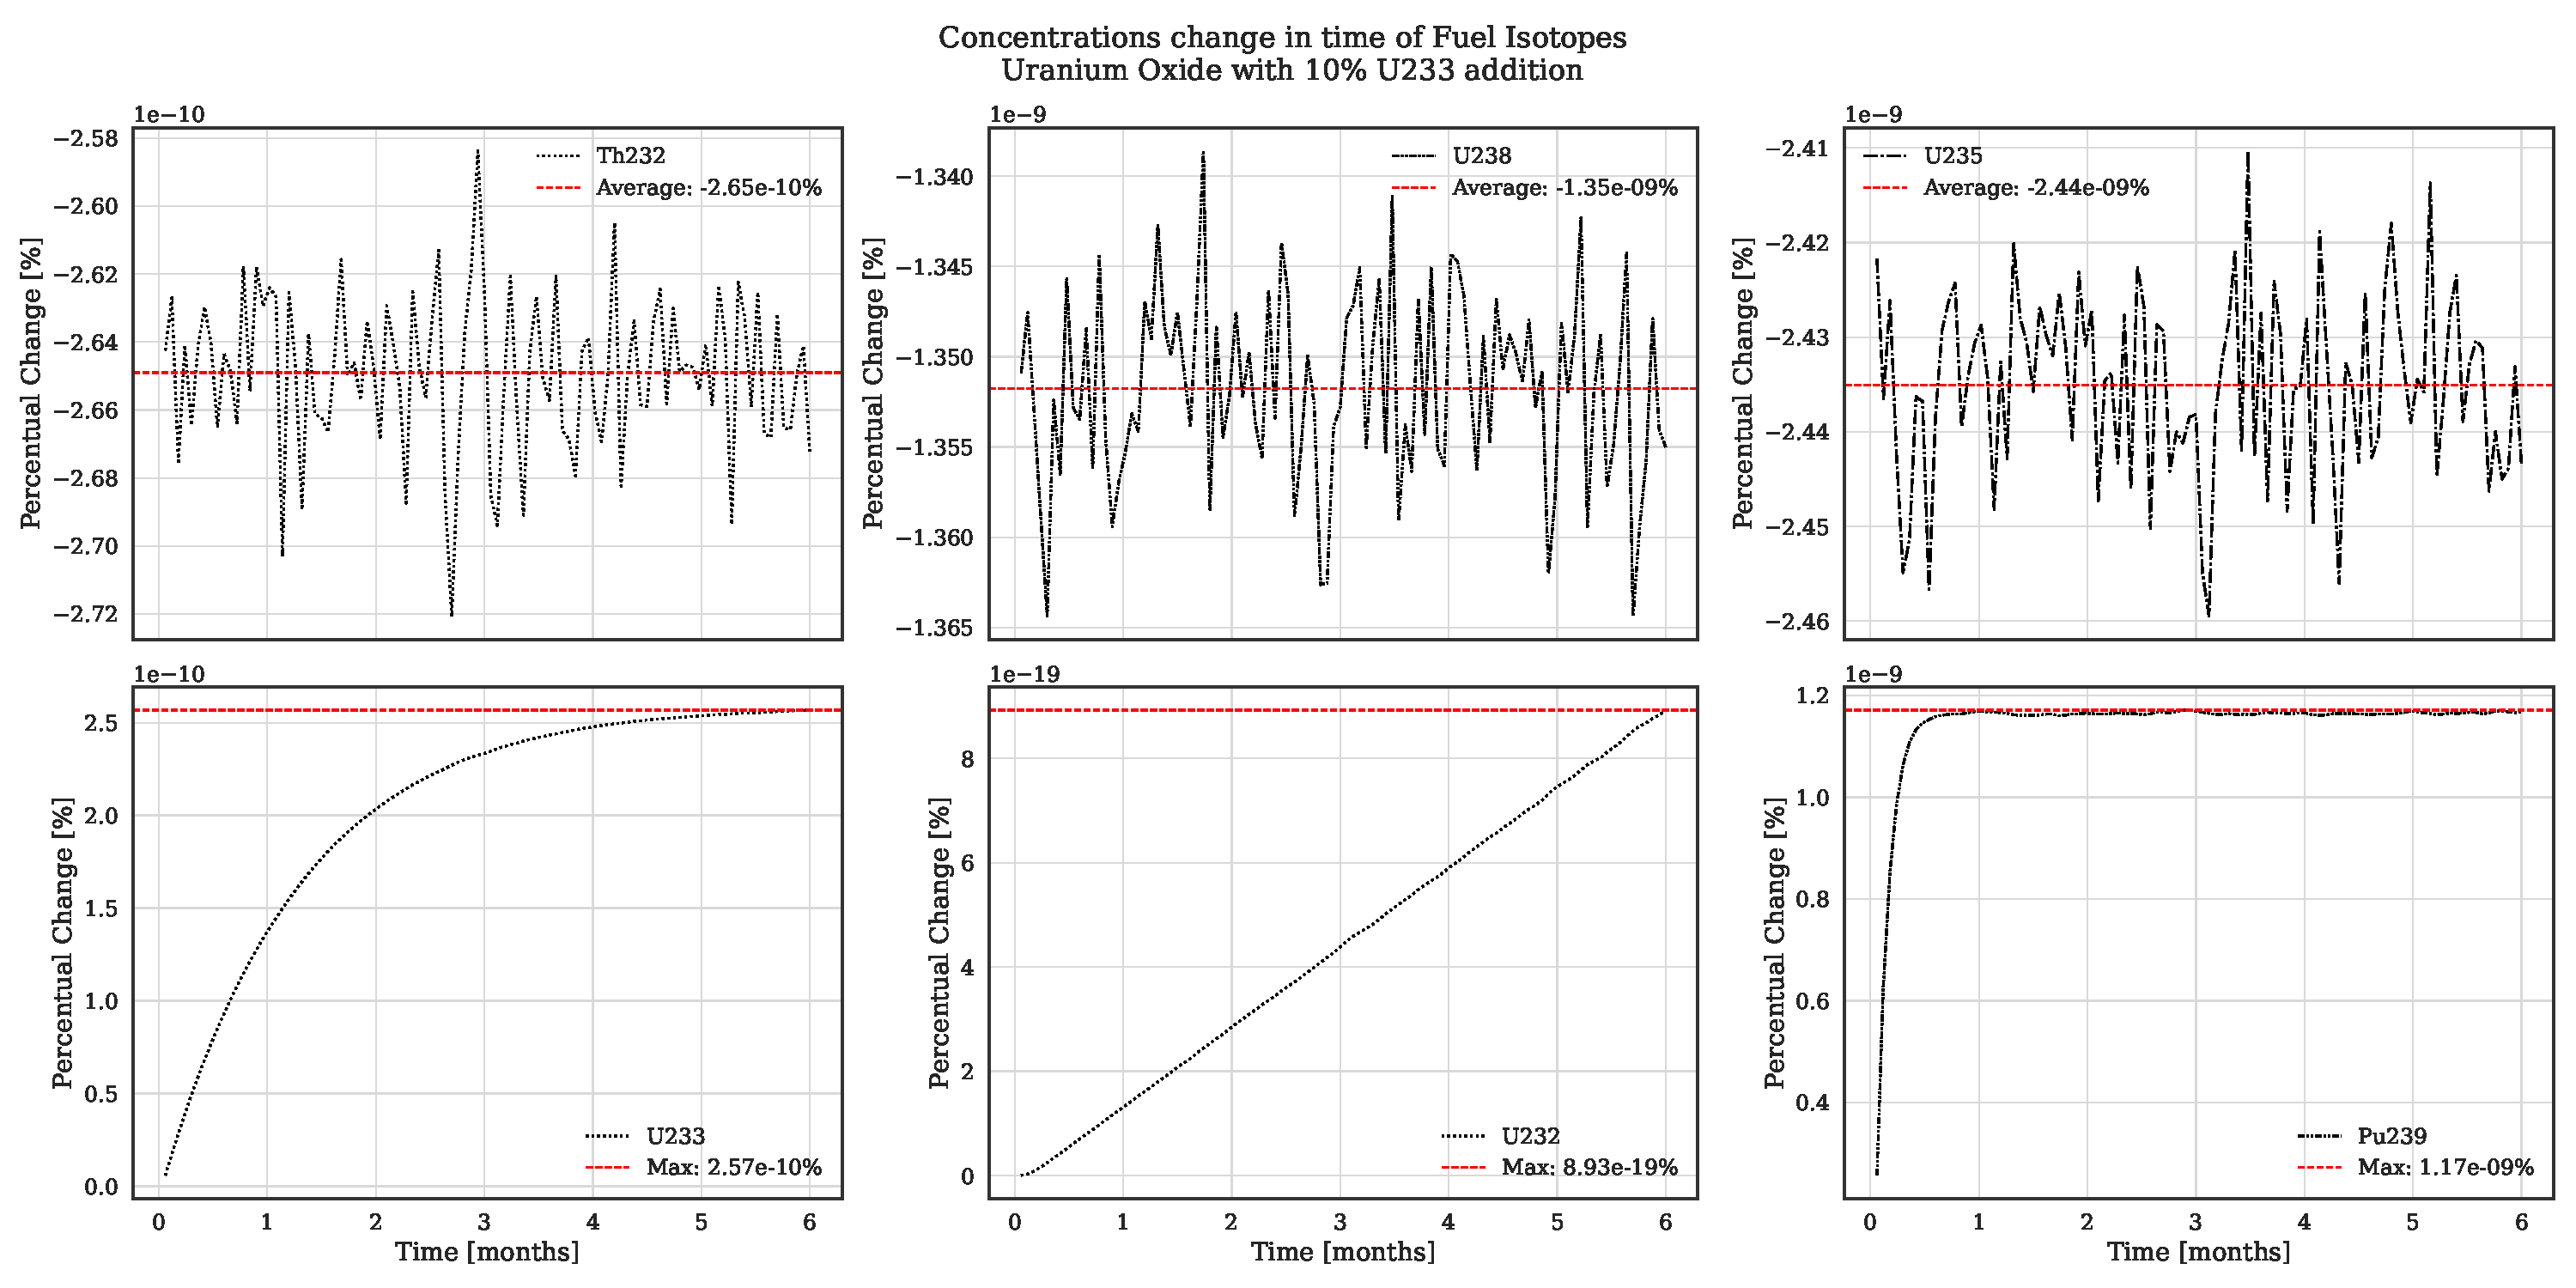
\includegraphics[width=1\textwidth]{Kap7/Figures_Kap7/percentual_change_th232_con_10.pdf}
    \caption{Percentage change of isotopes in the simulation of a PWR fuel assembly using UOX at \(10 \, \%\) thorium concentration.}
    \label{fig:th10}
\end{figure}

\begin{figure}[h]
    \centering
    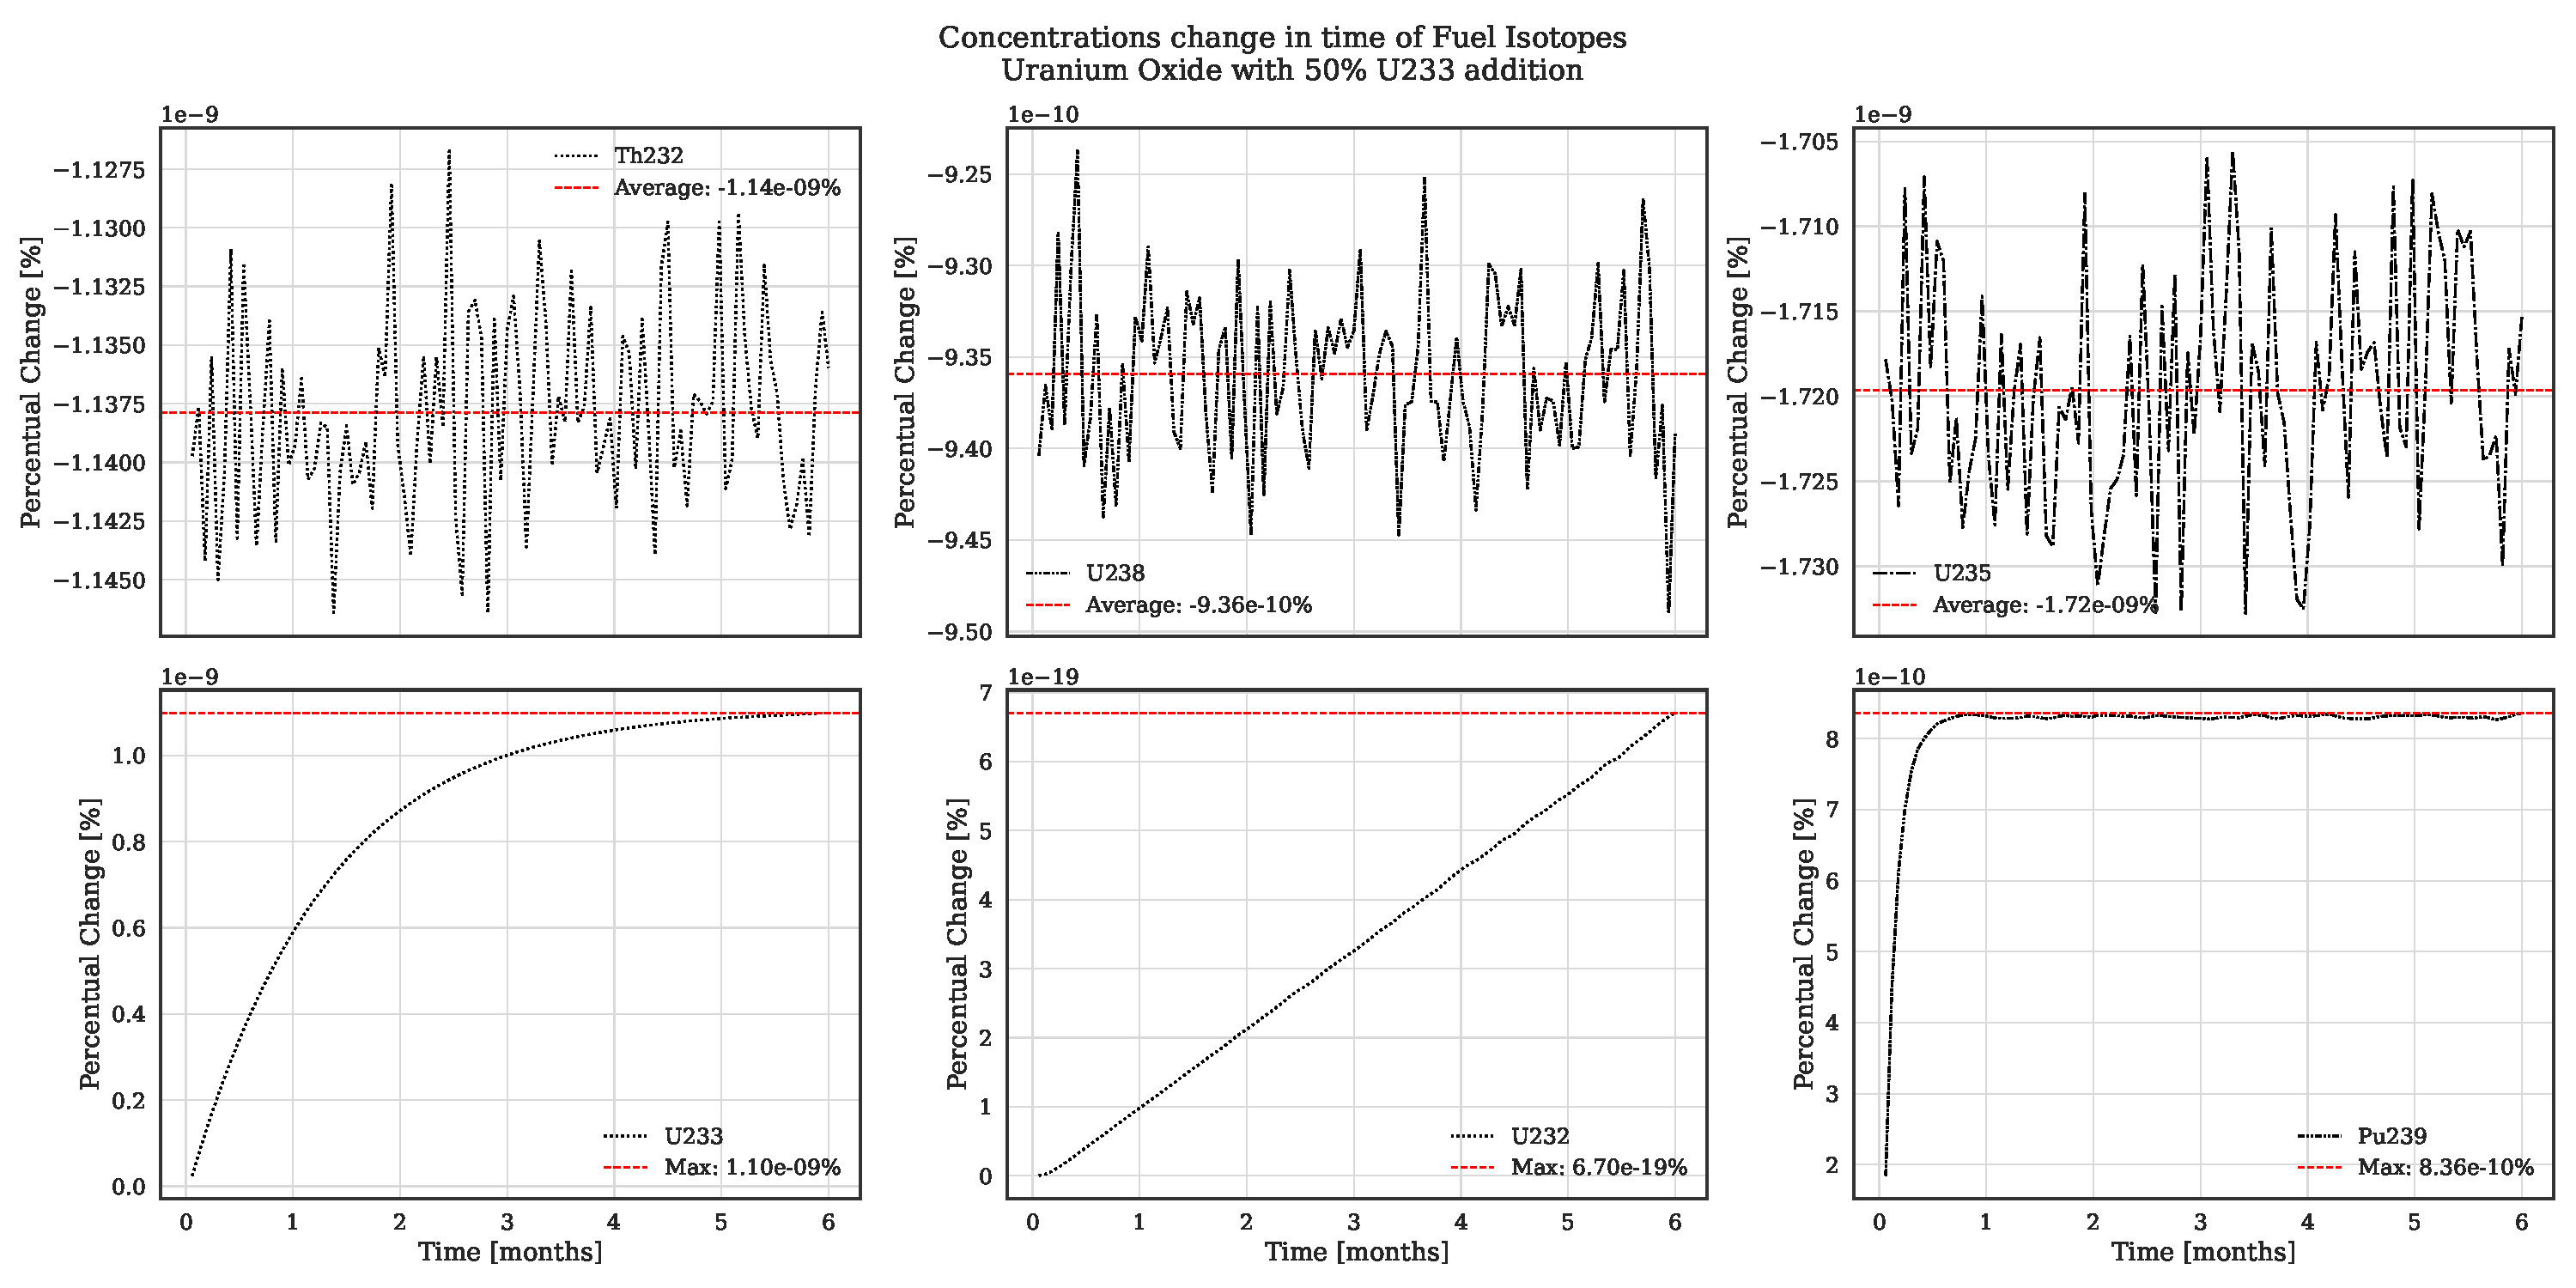
\includegraphics[width=1\textwidth]{Kap7/Figures_Kap7/percentual_change_th232_con_50.pdf}
    \caption{Percentage change of isotopes in the simulation of a PWR fuel assembly using UOX at \(50 \, \%\) thorium concentration.}
    \label{fig:th50}
\end{figure}

The simulations demonstrate that a \(10 \, \%\) thorium concentration in the fuel results in a good neutronic economy, aligning with previously reported results \cite{N_Improvement}. However, a \(50 \, \%\) thorium concentration leads to subcritical reactor behavior. This result are shown in figures \textbf{Fig.}\ref{fig:p_10} and \textbf{Fig.}\ref{fig:p_10}.

\begin{figure}[h]
    \centering
    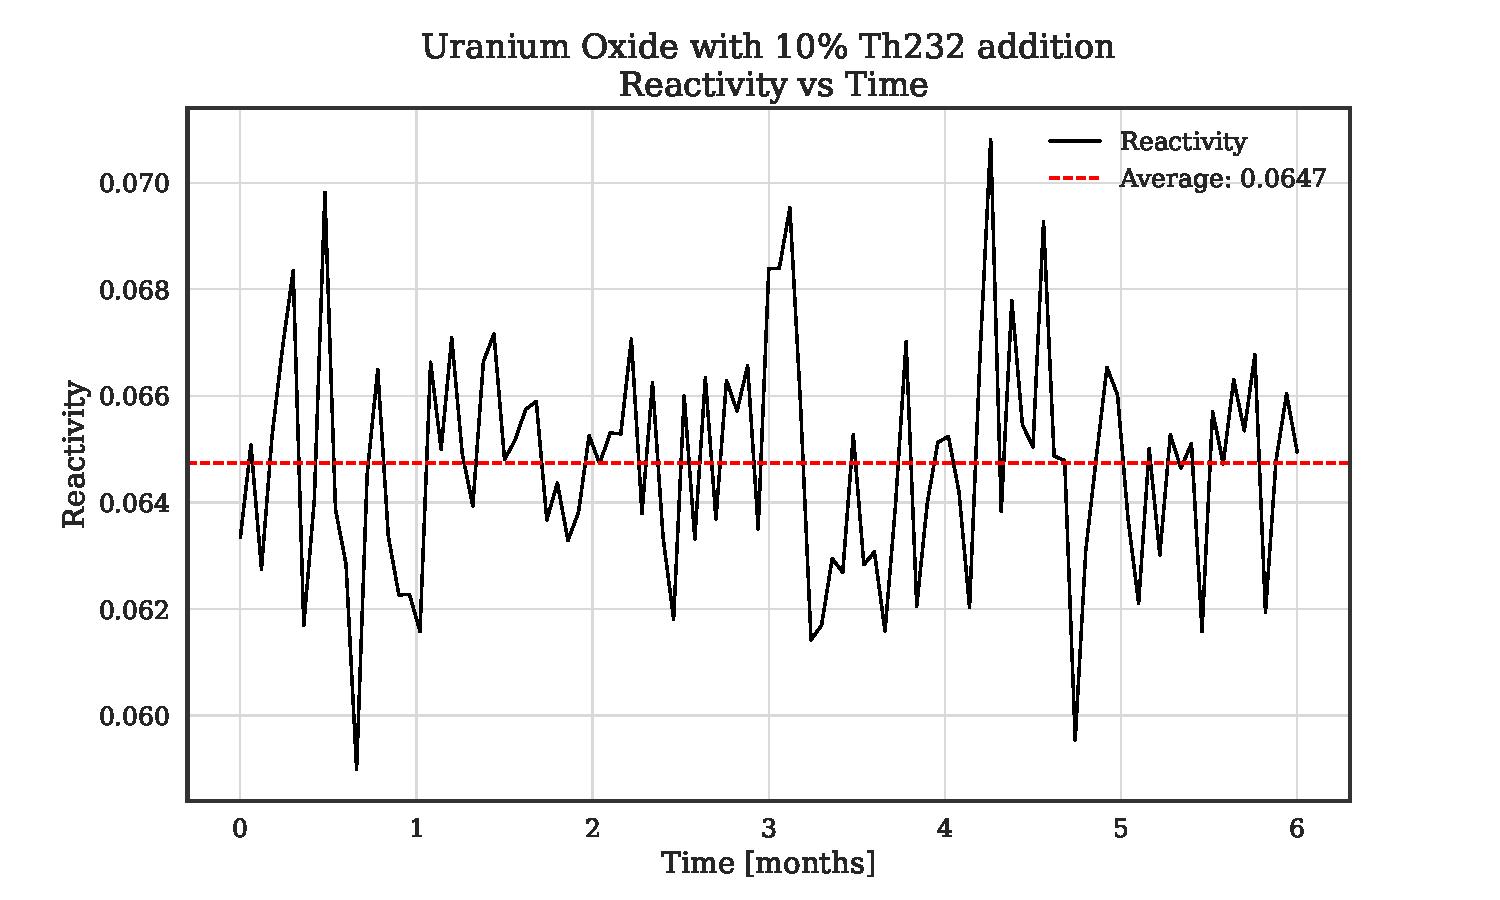
\includegraphics[width=0.75\textwidth, scale = 0.5]{Kap7/Figures_Kap7/Reactivity_vs_Time_UOX_10.pdf}
    \caption{Reactivity over time of the simulation of a PWR fuel assembly using UOX at \(10 \, \%\) thorium concentration.}
    \label{fig:p_10}
\end{figure}

\begin{figure}[h]
    \centering
    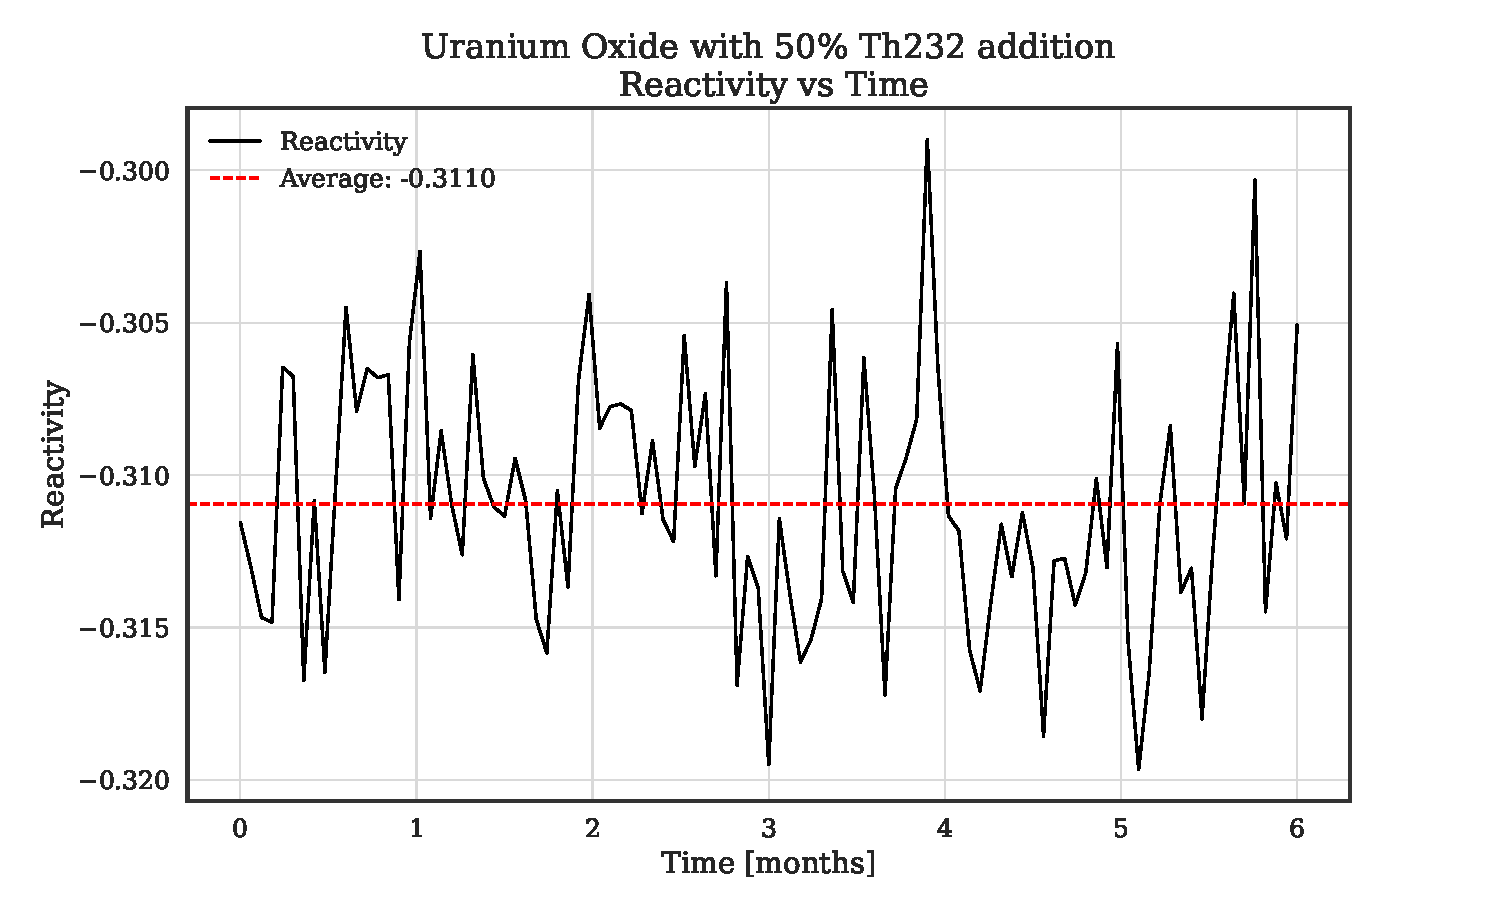
\includegraphics[width=0.75\textwidth, scale = 0.5]{Kap7/Figures_Kap7/Reactivity_vs_Time_UOX_50.pdf}
    \caption{Reactivity over time of the simulation of a PWR fuel assembly using UOX at \(50 \, \%\) thorium concentration.}
    \label{fig:p_10}
\end{figure}

Additional simulations were done to evaluate the behavior of thorium based fuel using thorium oxide and plutonium as seed isotope. The concentration of plutonium was set to \(10 \, \%\). The simulation shows that the fuel assembly reaches a critical state as well as it achieves a breeding ratio of \(\prescript{233}{}{U}\). However, the reactivity of the fuel assembly is higher than \(0\), this implies a more dangerous reactor behavior and additional technical issues to run it safetly. The results are shown in figures \textbf{Fig.}\ref{fig:th_pu}. The behavior of reactivity is show in figure \textbf{Fig.}\ref{fig:p_th_pu}.   

\begin{figure}[h]
    \centering
    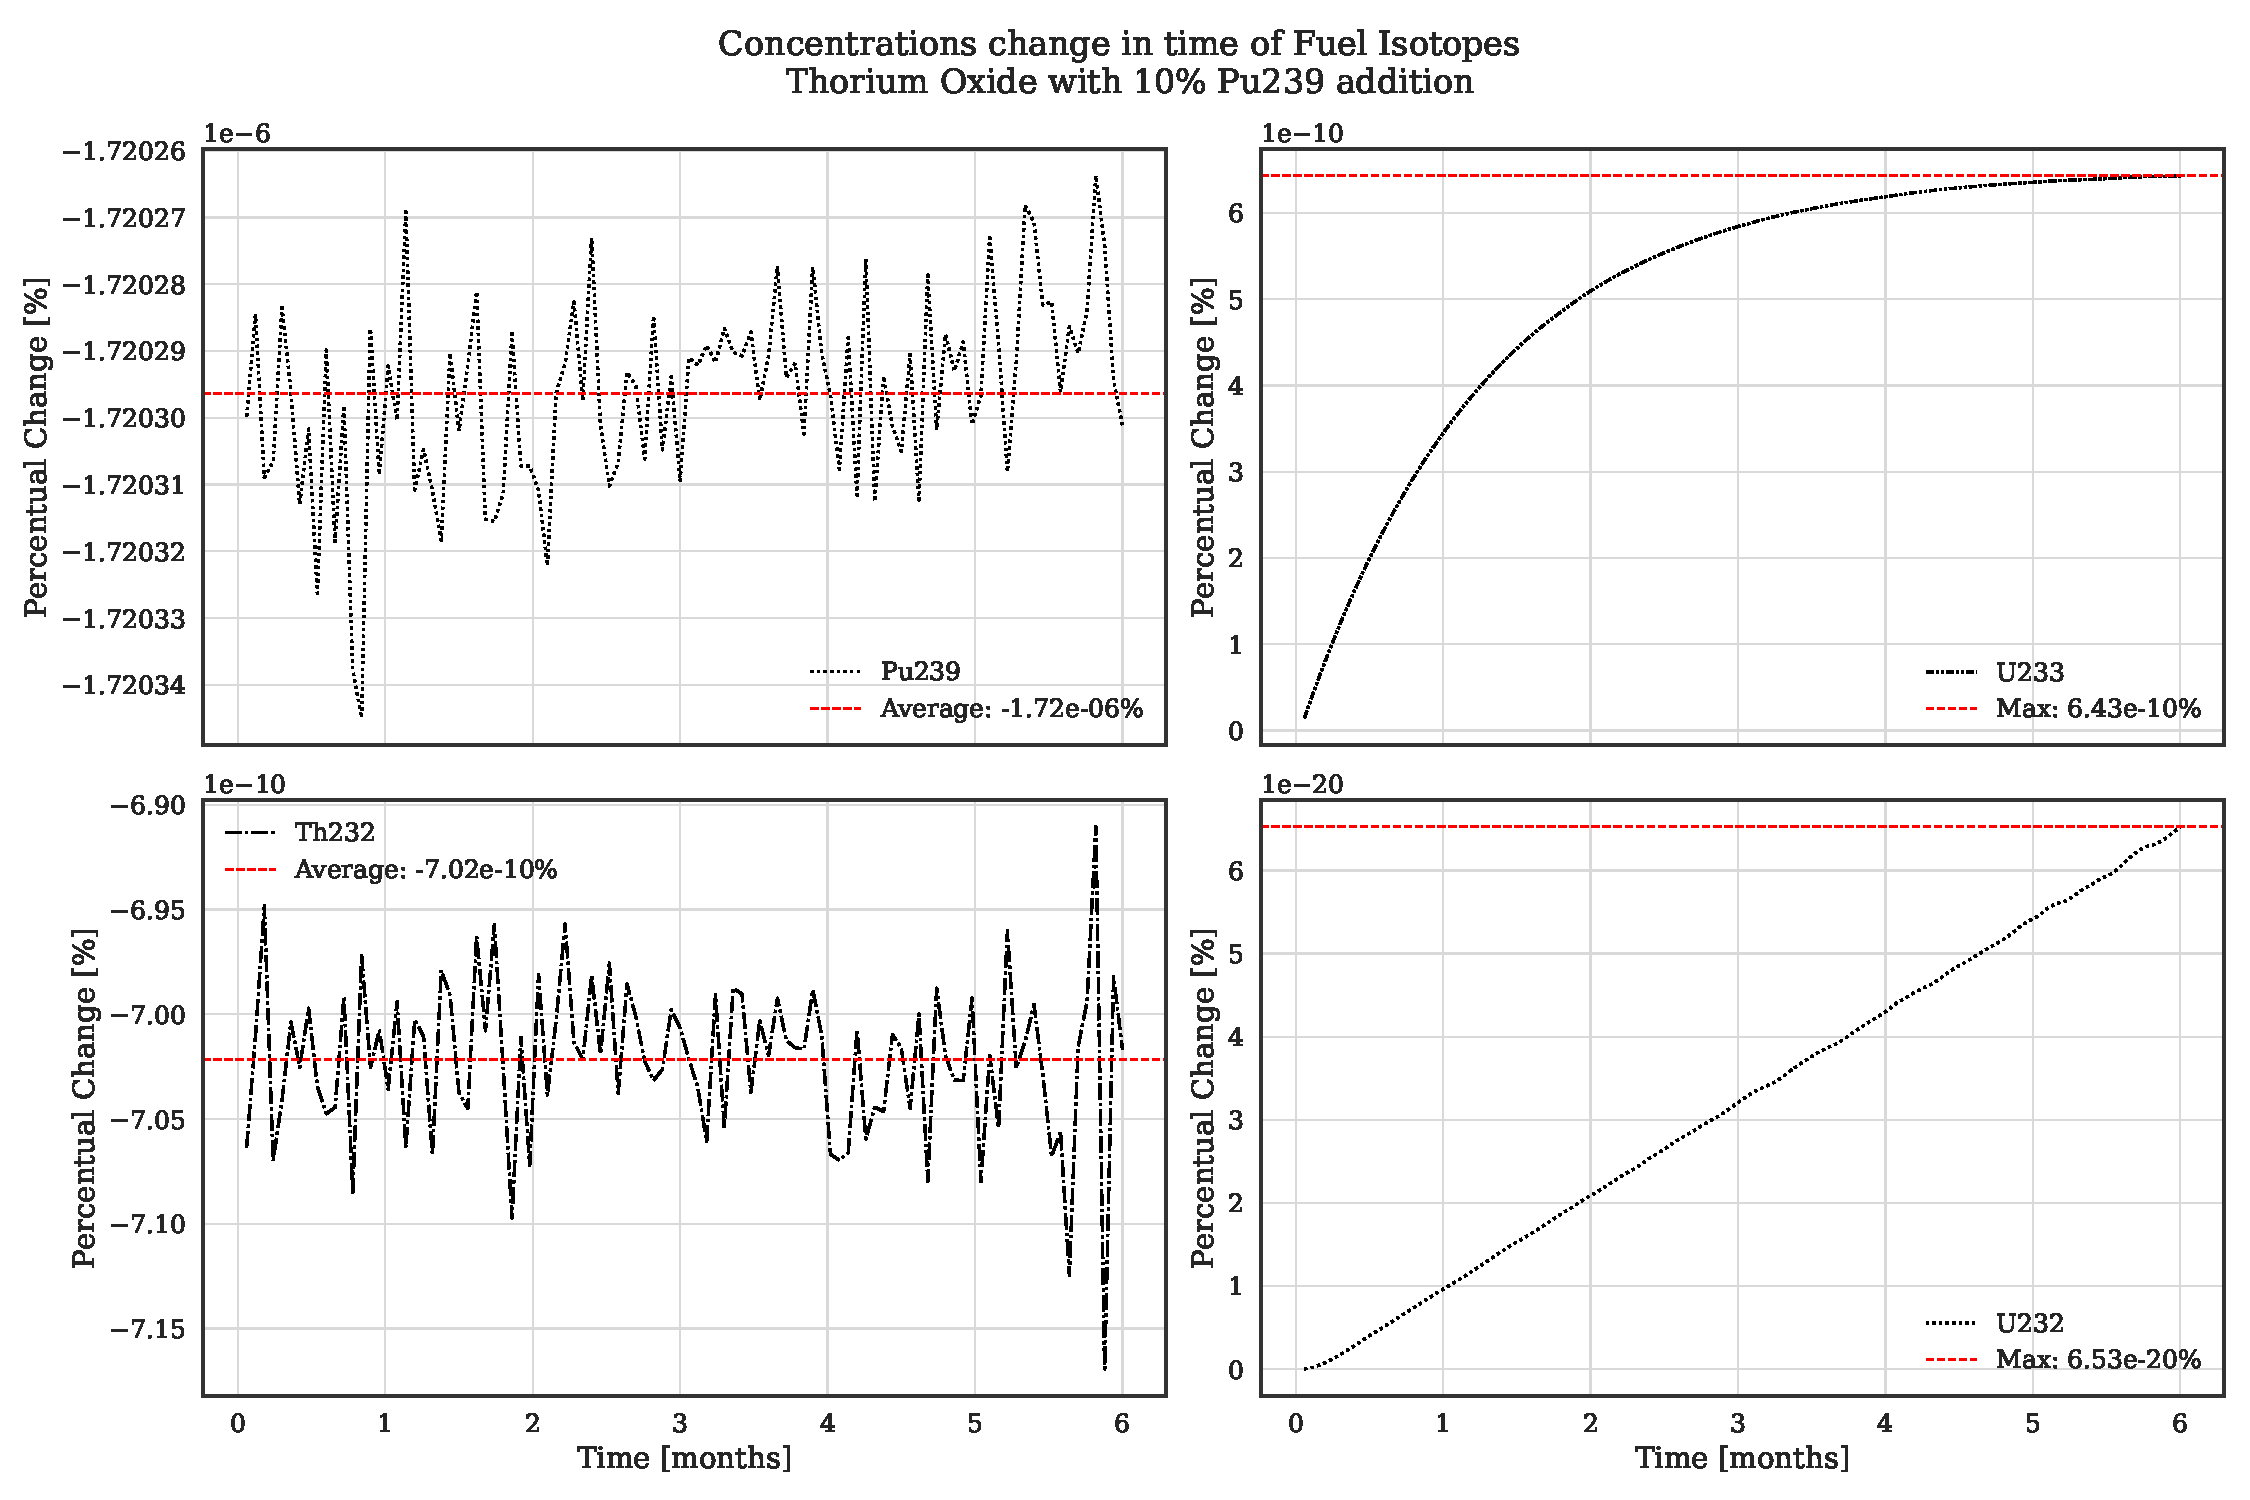
\includegraphics[width=1\textwidth]{Kap7/Figures_Kap7/percentual_change_th232_Pu239.pdf}
    \caption{Percentage change of isotopes in the simulation of a PWR fuel assembly using ThOX and \(10 \, \%\) plutonium concentration.}
    \label{fig:th_pu}
\end{figure}  


\begin{figure}[h]
    \centering
    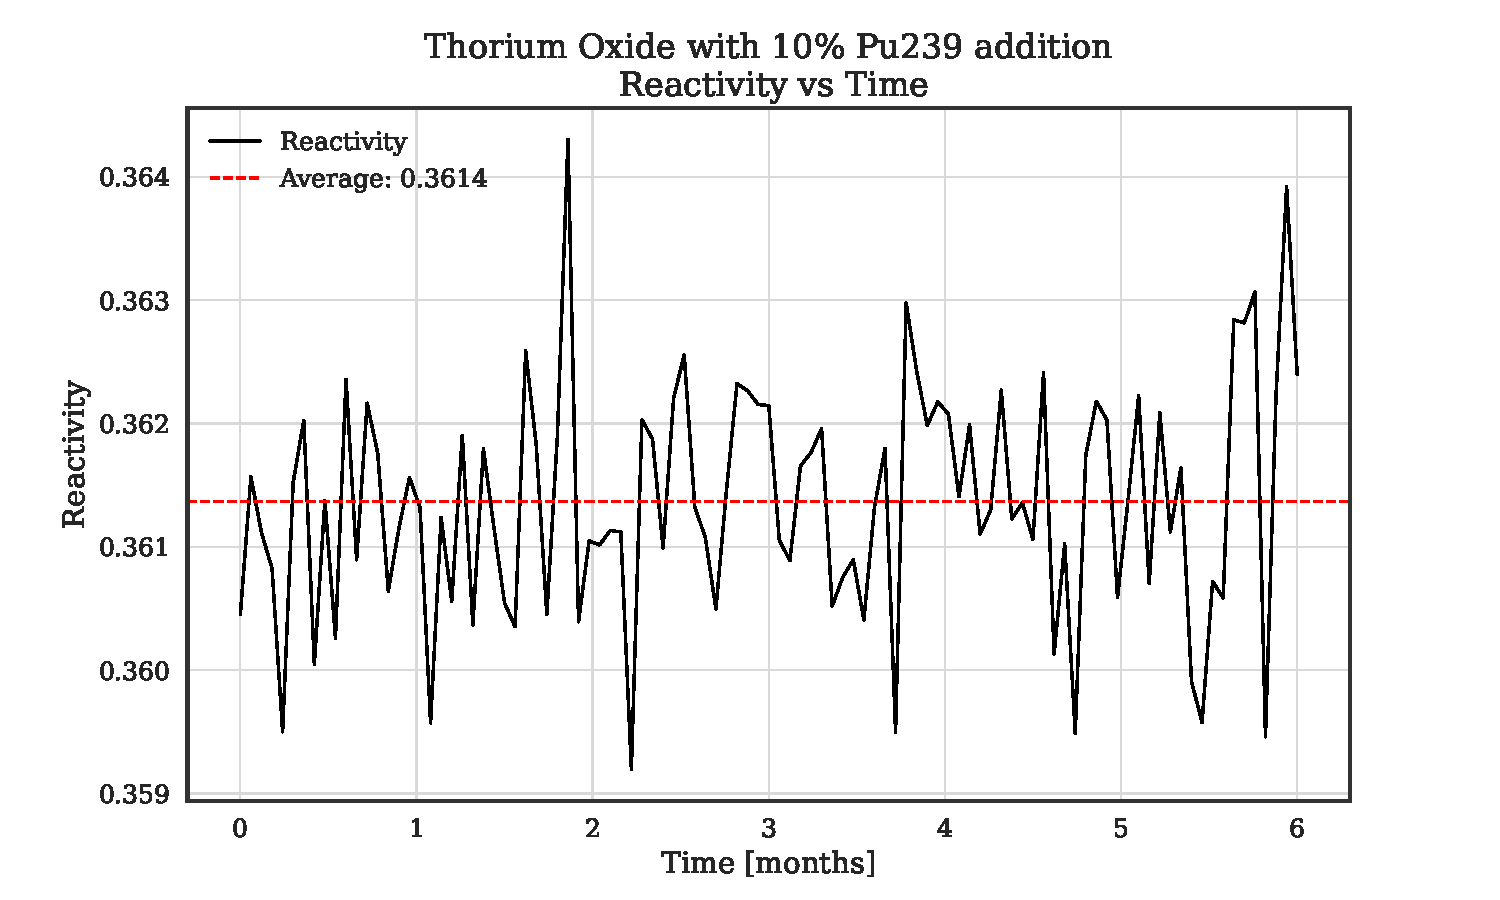
\includegraphics[width=0.75\textwidth, scale = 0.5]{Kap7/Figures_Kap7/Reactivity_vs_Time_ThOX_Pu10.pdf}
    \caption{Reactivity over time of the simulation of a PWR fuel assembly using ThOX and \(10 \, \%\) plutonium concentration.}
    \label{fig:p_th_pu}
\end{figure}

\section{Conclusion}
The simulations conducted in this project provide valuable insights into the behavior of thorium-based nuclear fuels in a Pressurized Water Reactor (PWR). The results demonstrate that thorium oxide (ThOX) with uranium-233 (\(\prescript{233}{}{U}\)) at concentrations of \(5 \, \%\) and \(10 \, \%\) can achieve breeding. However, the stability of breeding is achieved much later compared to plutonium-239 (\(\prescript{239}{}{Pu}\)). This delay is due to the slower breeding process of \(\prescript{233}{}{U}\) from \(\prescript{232}{}{Th}\) compared to the breeding of \(\prescript{239}{}{Pu}\) from \(\prescript{238}{}{U}\).

Additionally, the simulations show an improvement in neutronic economy with thorium-based fuels. This improvement is characterized by a reduction in excess reactivity at the beginning of the fuel cycle, which helps to minimize the initial reactivity spike and associated control challenges. Furthermore, the simulations indicate that thorium-based fuels can maintain criticality towards the end of the fuel cycle, ensuring a more stable and efficient reactor operation over time.Overall, the use of ThOX with \(\prescript{233}{}{U}\) not only supports breeding but also enhances the neutronic performance of the reactor by providing a more balanced reactivity profile throughout the fuel cycle.

The simulation results for ThOX with \(10 \, \%\) thorium concentration (\textbf{Fig.}\ref{fig:th10}) show a good neutronic economy, aligning with previously reported results. However, increasing the thorium concentration to \(50 \, \%\) leads to subcritical reactor behavior (\textbf{Fig.}\ref{fig:th50}). This indicates that while thorium can be beneficial in certain concentrations, higher concentrations may pose challenges for maintaining criticality.

Additionally, the simulation of ThOX with \(10 \, \%\) plutonium concentration (\textbf{Fig.}\ref{fig:th_pu}) shows that the fuel assembly reaches a critical state and achieves a breeding ratio of \(\prescript{233}{}{U}\). However, the higher reactivity of the fuel assembly implies a more dangerous reactor behavior and additional technical issues to ensure safe operation (\textbf{Fig.}\ref{fig:p_th_pu}).

For comparison, the simulation using uranium oxide (UOX) as a reference (\textbf{Fig.}\ref{fig:uo2}) highlights the differences in behavior between traditional uranium-based fuels and thorium-based fuels. The results indicate that while UOX can maintain criticality, the breeding capabilities of thorium-based fuels offer potential advantages for long-term sustainability and fuel utilization.

In conclusion, thorium-based fuels, particularly ThOX with \(\prescript{233}{}{U}\), show promise for use in PWRs. However, while the chain reaction can be sustained with these fuels, the simulations indicate that achieving criticality is challenging, since the reactivity was about \(0\)(), and it was not possible to achieve a stable breeding of \(\prescript{233}{}{U}\). Careful consideration of fuel composition and concentration is necessary to balance breeding capabilities and reactor safety. Further research and optimization are required to fully realize the potential of thorium as a sustainable nuclear fuel.


\chapter{Present and future of Thorium}

The research and simulations conducted in this project provide valuable insights into the potential and challenges of using thorium-based nuclear fuels in PWRs. The thorium fuel cycle, with its unique properties and benefits, presents a promising alternative to traditional uranium-based fuels. However, several technical and operational challenges must be addressed to fully realize its potential.

\section{Thorium Fuel Cycle}

The thorium fuel cycle offers several advantages over the conventional uranium fuel cycle. Thorium is more abundant than uranium, and its use in nuclear reactors can lead to higher efficiency harvesting energy from the fuel. The chemical stability and higher thermal conductivity of thorium dioxide (\(ThO_2\)) compared to uranium dioxide (\(UO_2\)) make it a more suitable material for nuclear fuel, potentially improving in-pile performance and long-term storage of irradiated fuel.

The intrinsic proliferation resistance of the thorium fuel cycle, due to the formation of \(\prescript{232}{}{U}\) and its strong gamma emissions, makes it less attractive for the production of nuclear weapons. This adds a significant layer of security in the context of nuclear non-proliferation.

\section{Simulation Results}

The simulations conducted using OpenMC provided detailed insights into the behavior of thorium-based fuels in a PWR. The results demonstrated that thorium oxide (ThOX) with uranium-233 (\(\prescript{233}{}{U}\)) at concentrations of \(5 \, \%\) and \(10 \, \%\) can not achieve breeding. Thi is consistent with previous studies that have shown that breeding with ThOX and \(\prescript{233}{}{U}\) is challenging in thermal reactors \cite{roadmap}. However, it may be possible to achieve breeding with more sophisticated simulations and optimization of fuel composition and core configuration.

Simulations also show that using \(ThO_2\) in combination with \(\prescript{239}{}{Pu}\) a breeding ration can be achieved. However, the saturation poitn of the breeding process is achieved much later compared to \(\prescript{239}{}{Pu}\) breeding using uranium oxide. This delay is due to the slower breeding process of \(\prescript{233}{}{U}\) from \(\prescript{232}{}{Th}\) compared to the breeding of \(\prescript{239}{}{Pu}\) from \(\prescript{238}{}{U}\).

The simulations also showed an improvement in neutronic economy with thorium-based fuels. This improvement is characterized by a reduction in excess reactivity at the beginning of the fuel cycle, which helps to minimize the initial reactivity spike and associated control challenges. Furthermore, the simulations indicate that thorium-based fuels can maintain criticality towards the end of the fuel cycle, ensuring a more stable and efficient reactor operation over time. This behavior is consistent with the finding in \textbf{Ref.}\cite{LAU201248}

\section{Challenges and Future Research}

Despite the promising results, several challenges remain in the implementation of thorium-based fuels. Achieving and maintaining criticality with ThOX and \(\prescript{233}{}{U}\) requires careful consideration of fuel composition and concentration. The simulations indicated that higher thorium concentrations could lead to subcritical reactor behavior.

Additionally, achieving optimal breeding ratios with ThOX and \(\prescript{233}{}{U}\) may require more sophisticated designs in the fuel lattice and core configuration. The results suggest that optimizing these parameters is crucial for enhancing the performance and safety of thorium-based fuels.

Further research and development are necessary to address these challenges and fully realize the potential of thorium as a sustainable nuclear fuel. This includes exploring advanced reactor designs, such as Molten Salt Reactors (MSRs), which offer several advantages over traditional Light Water Reactors (LWRs), including higher thermal efficiency, lower proliferation risk, and improved safety features.

Additionally, it is essential to develop fuel reprocessing and recycling technologies to economically extract and reuse valuable fissile materials from irradiated thorium-based fuels. This will help reduce the volume of radioactive waste and maximize the energy potential of thorium resources.

Finally, regulatory and policy frameworks must be established to support the deployment of thorium-based fuels and ensure their safe and secure operation. This includes addressing licensing and permitting requirements, as well as establishing international cooperation and standards for the use of thorium in nuclear energy production.

\section{Conclusion}

In conclusion, thorium-based fuels, particularly ThOX with \(\prescript{233}{}{U}\), show significant promise for use in PWRs. The simulations conducted in this project provide valuable insights into the behavior of these fuels and highlight the potential benefits and challenges associated with their use. While the thorium fuel cycle offers several advantages, including higher conversion ratios, improved thermal properties, and intrinsic proliferation resistance, achieving and maintaining criticality presents challenges that require further research and optimization.

The future of thorium-based nuclear fuels looks promising, with ongoing research and development efforts aimed at overcoming the technical and operational challenges. By addressing these challenges, thorium-based fuels could play a crucial role in the future of sustainable and safe nuclear energy production.
\appendix

\chapter{Simulation Results}

Here are listed additional plots generated from the simulations. The plots show the percentage change of isotopes in the simulation with different thorium concentrations. 

\begin{figure}[h]
    \centering
    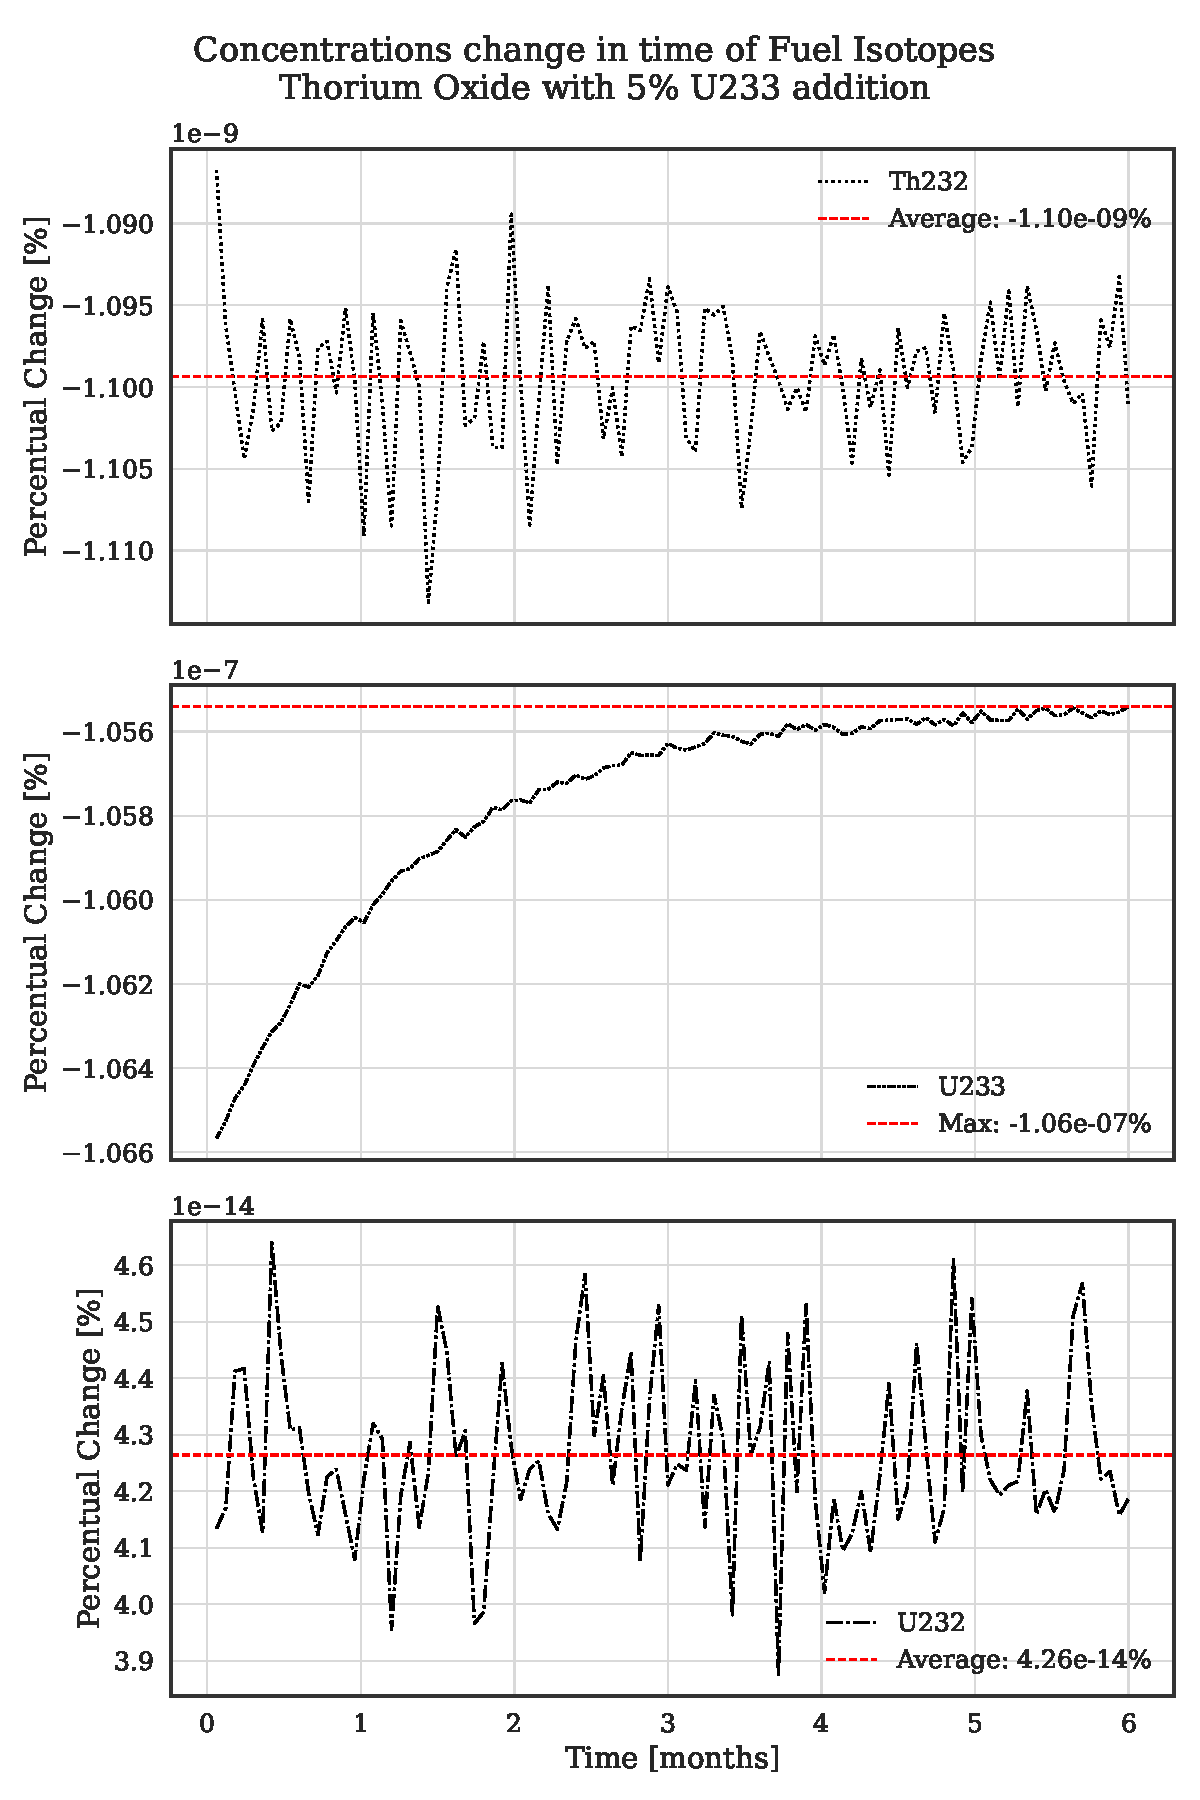
\includegraphics[width=0.75\textwidth, height=0.75\textheight]{Kap7/Figures_Kap7/percentual_change_th232_U233_5.pdf}
    \caption{Percentage change of isotopes in the simulation of a PWR fuel assembly using ThOX at \(5 \, \%\) \(\prescript{233}{}{U}\) concentration.}
    \label{fig:th_u233_5}
\end{figure}

\begin{figure}[h]
    \centering
    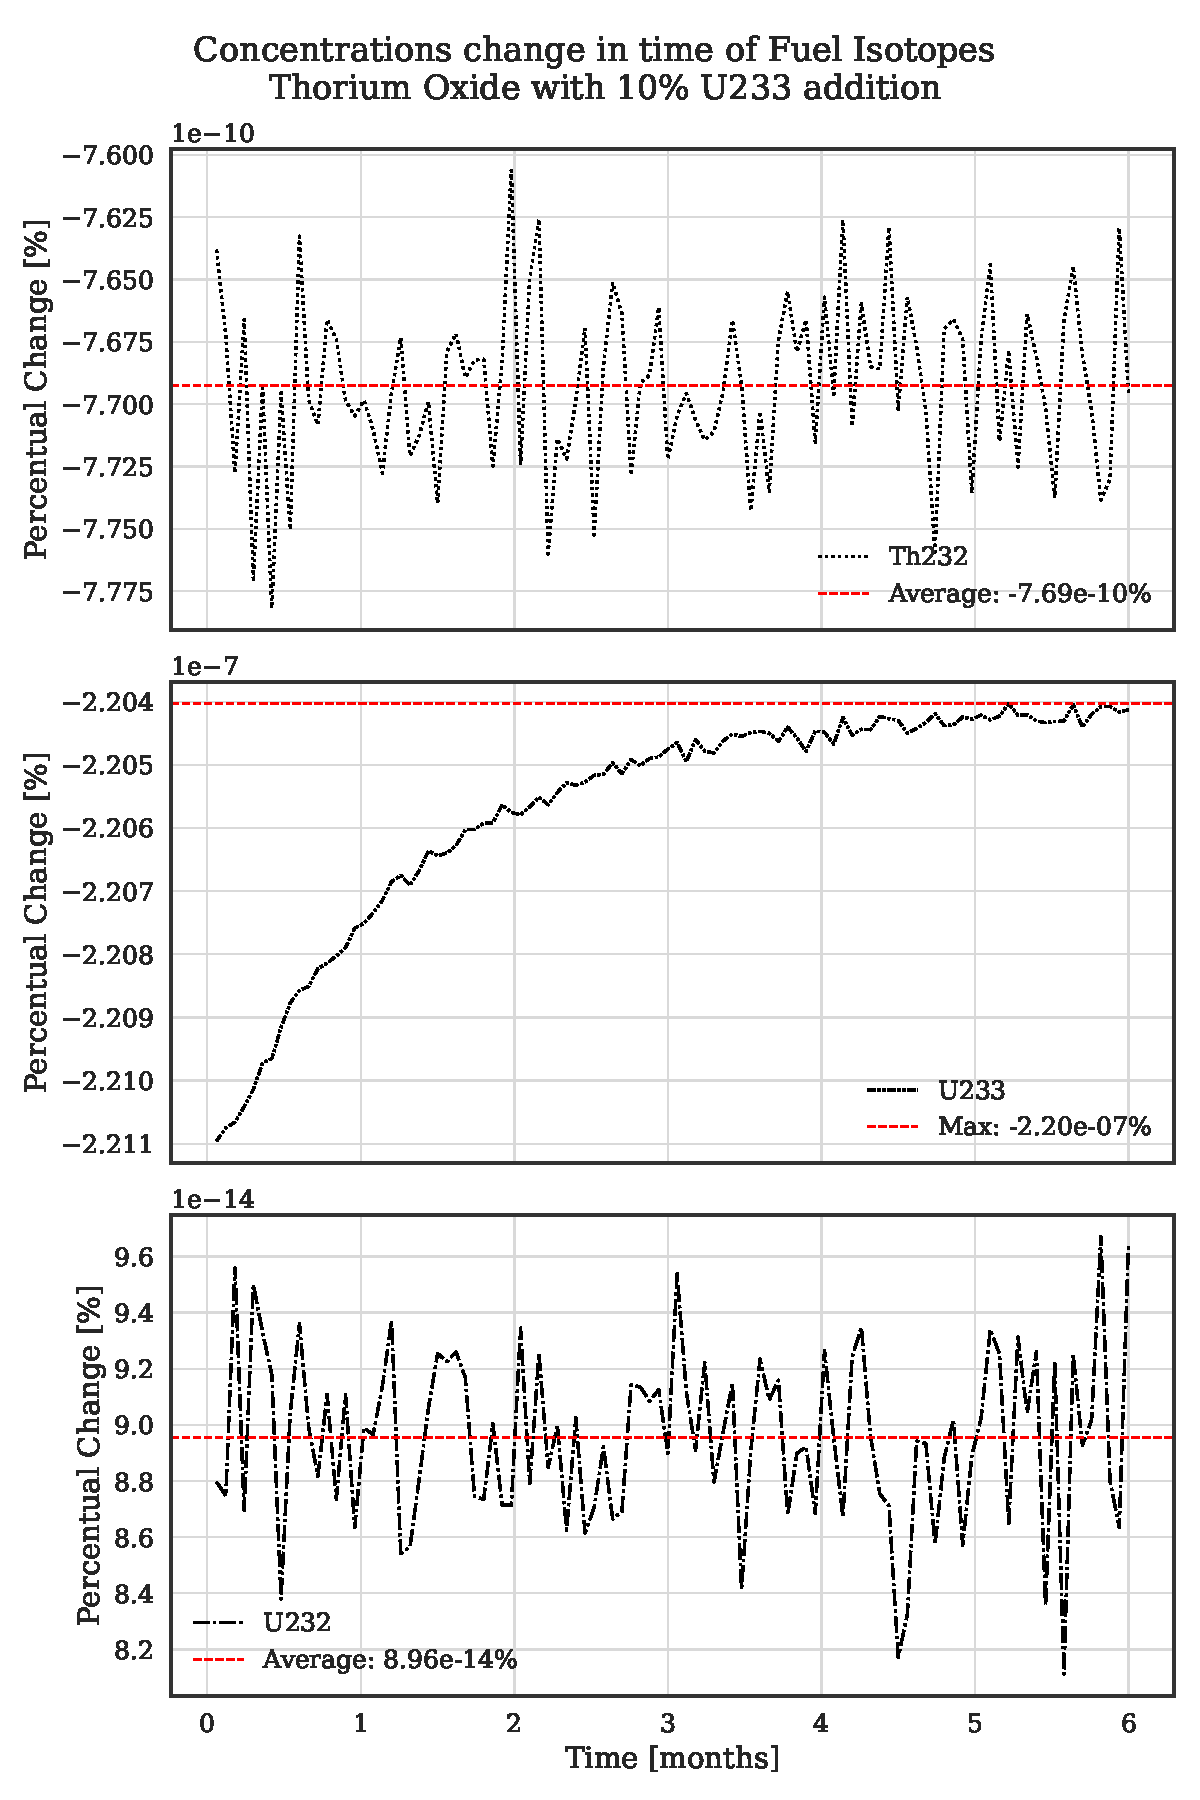
\includegraphics[width=0.75\textwidth, height=0.75\textheight]{Kap7/Figures_Kap7/percentual_change_th232_U233_10.pdf}
    \caption{Percentage change of isotopes in the simulation of a PWR fuel assembly using ThOX at \(10 \, \%\) \(\prescript{233}{}{U}\) concentration.}
    \label{fig:th_u233_10}
\end{figure}


 Reactivity behavior of the fuel assemblies during the simulation. The reactivity is calculated as in \textbf{Eq} (\ref{eq:def_reactivity}). It is noticeable that the reactivity of UOX, used as reference, is higher than \(0\). This is because the simulation is run from the beginning of the cycle, where it is needed this reactivity excess to ensure criticality of the reactor through the whole cycle.

\begin{figure}
    \centering
    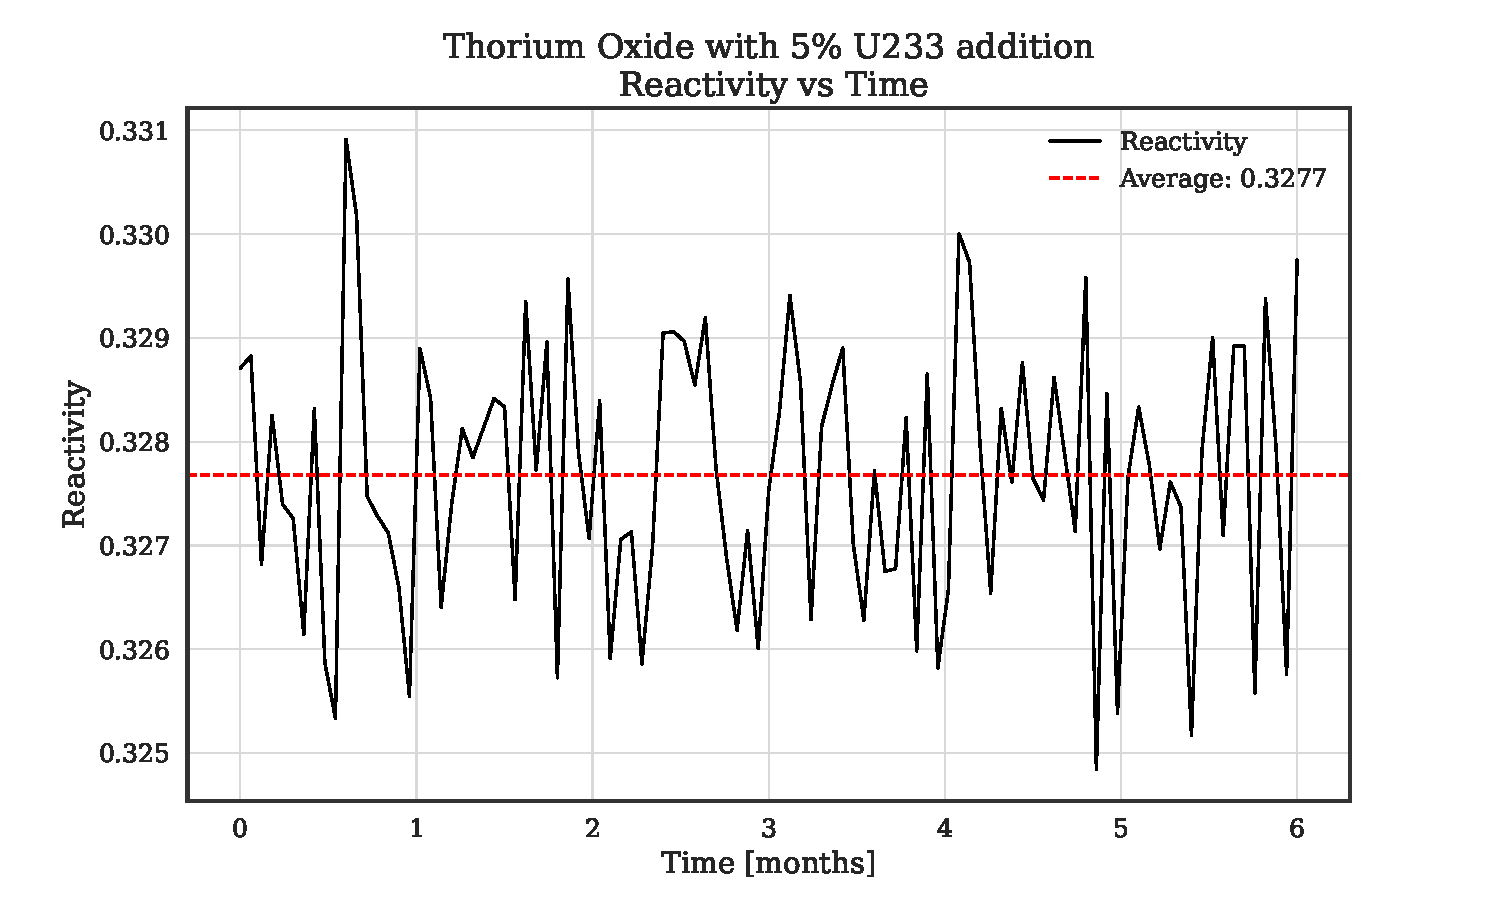
\includegraphics[width=0.75\textwidth, scale=0.75]{Kap7/Figures_Kap7/Reactivity_vs_Time_ThOX_U233_5.pdf}
    \caption{Reactivity of the simulation of a PWR fuel assembly using ThOX at \(5 \, \%\) \(\prescript{233}{}{U}\) concentration.}
    \label{fig:reactivity_th_u233_5}
\end{figure}

\begin{figure}
    \centering
    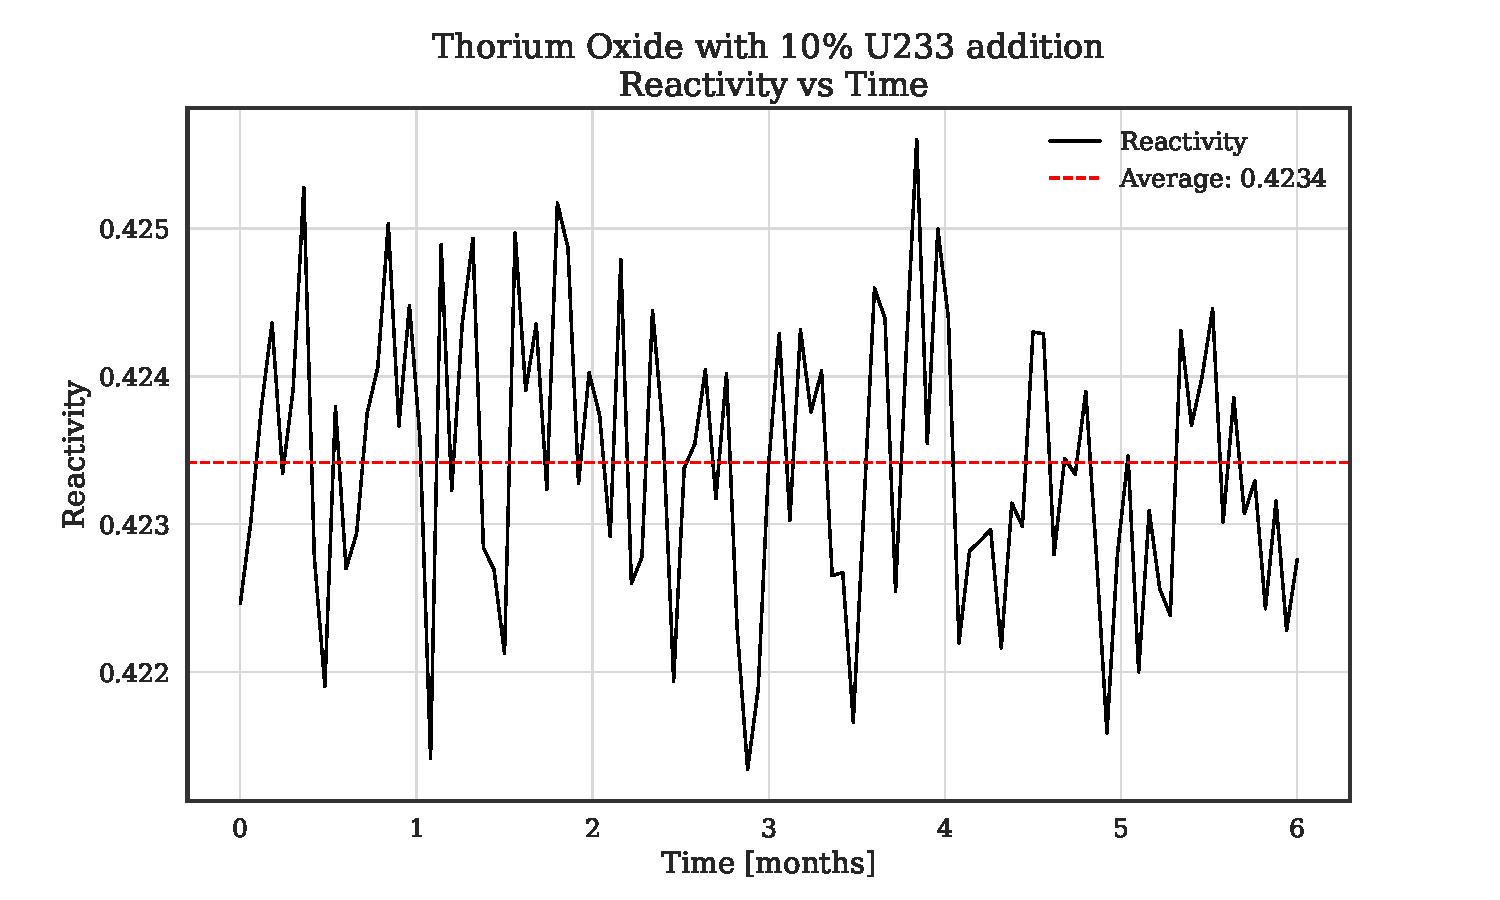
\includegraphics[width=0.75\textwidth, scale=0.75]{Kap7/Figures_Kap7/Reactivity_vs_Time_ThOX_U233_10.pdf}
    \caption{Reactivity of the simulation of a PWR fuel assembly using ThOX at \(10 \, \%\) \(\prescript{233}{}{U}\) concentration.}
    \label{fig:reactivity_th_u233_10}   
\end{figure}

\begin{figure}
    \centering
    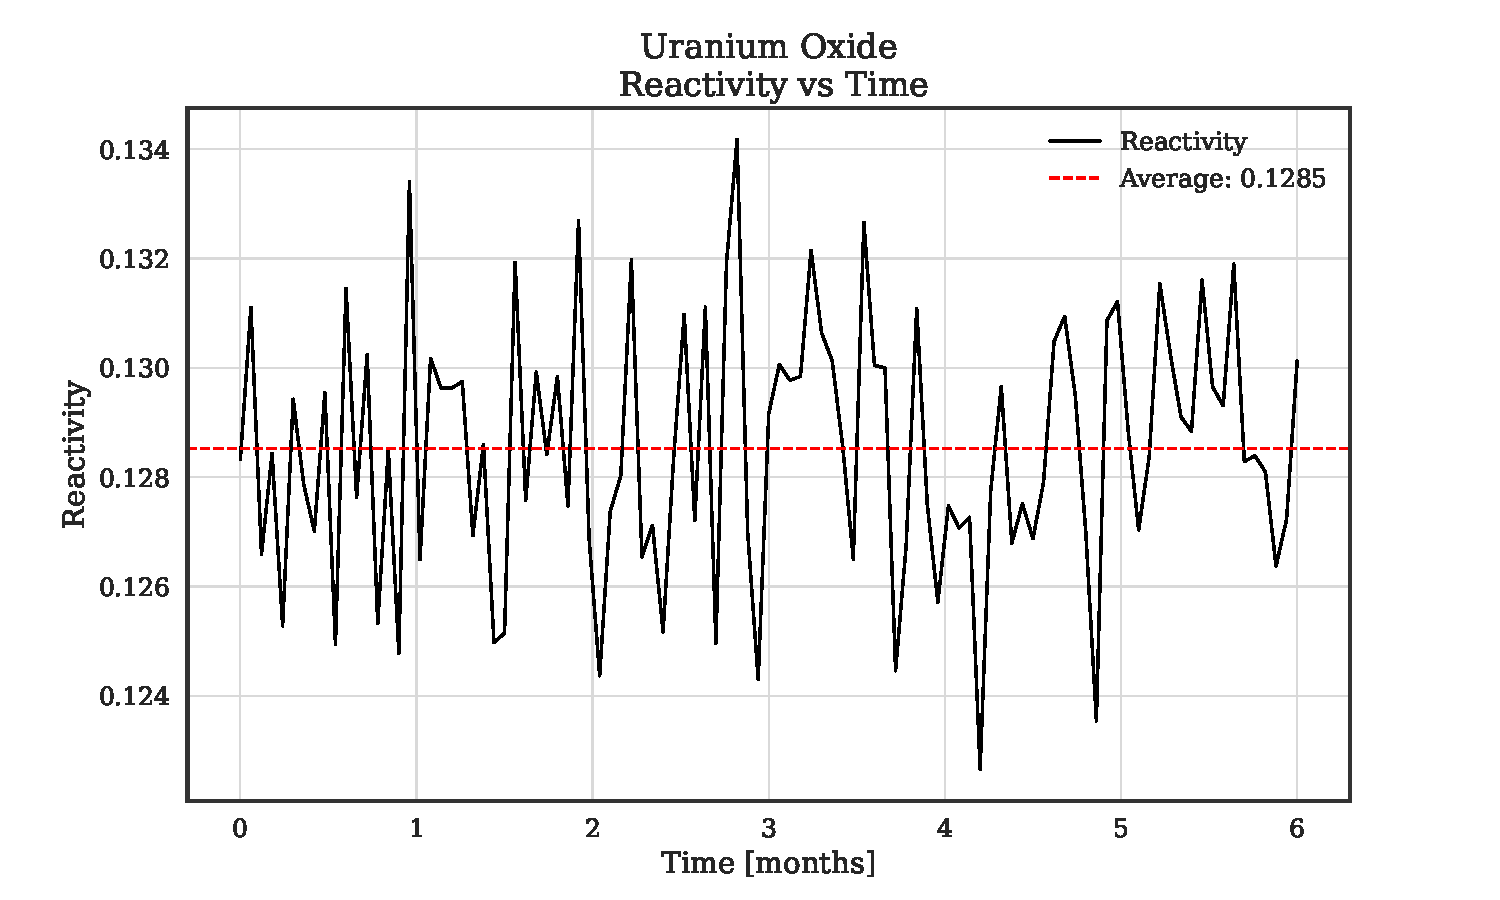
\includegraphics[width=0.75\textwidth, scale=0.75]{Kap7/Figures_Kap7/Reactivity_vs_Time_UOX.pdf}
    \caption{Reactivity of the simulation of a PWR fuel assembly using UOX.}
    \label{fig:reactivity_uox}
\end{figure}

\addcontentsline{toc}{chapter}{Bibliography}
%\bibliographystyle{IEEEtran} 
%\bibliography{BibliMSc,Kap1/BibtexChap1,Kap2/BibtexChap2,Kap3/BibtexChap3,Kap4/BibtexChap4,Kap5/BibtexChap5}

\printbibliography
\end{document}